%% LaTeX2e class for student theses
%% thesis.tex
%% 
%% Karlsruhe Institute of Technology
%% Institute for Program Structures and Data Organization
%% Chair for Software Design and Quality (SDQ)
%%
%% Dr.-Ing. Erik Burger
%% burger@kit.edu
%%
%% Version 1.3.2, 2017-08-01

%% Available page modes: oneside, twoside
%% Available languages: english, ngerman
%% Available modes: draft, final (see README)
\documentclass[twoside, english]{sdqthesis}
\graphicspath{Figures/}
\usepackage{float}
\usepackage{amsmath}
\usepackage[colorinlistoftodos,prependcaption]{todonotes}
\DeclareMathOperator*{\argmax}{arg\,max}
\DeclareMathOperator*{\argmin}{arg\,min}
\usepackage{verbatim}  % Needed for the "comment" environment to make LaTeX comments
\usepackage{vector}  % Allows "\bvec{}" and "\buvec{}" for "blackboard" style bold vectors in maths
\usepackage{colortbl}
%\usepackage[urlcolor=blue, colorlinks=true, linkcolor=black, citecolor=blue]{hyperref}  % Colours hyperlinks in blue, but this can be distracting if there are many links.
\usepackage{pgfplots}
\usepackage{subcaption}
\usepackage{csquotes}
\usepackage{algorithm}

\usepackage{alphalph}
\renewcommand*{\thesubfigure}{%
\alphalph{\value{subfigure}}%
}%
\newcommand \dsingle {d_\text{min}}
\newcommand \dcomplete {d_\text{max}}
\newcommand \daverage {d_\text{avg}}
\newcommand \dsc {\mathcal{D}_\text{SC}}
\newcommand \dsa {\mathcal{D}_\text{SA}}
\newcommand \dac {\mathcal{D}_\text{AC}}

\newcommand \alo {\alpha_\text{lo}}
\newcommand \ahi {\alpha_\text{hi}}
\newcommand \blo {\beta_\text{lo}}
\newcommand \bhi {\beta_\text{hi}}

\newcommand \metric {\operatorname{d}}
\newcommand \metricp [1]{\operatorname{d_{#1}}}
\newcommand \dbeta {\metricp{\beta}}
\newcommand \dOne {\metricp{1}}
\newcommand \dZero {\metricp{0}}

\newcommand \cmetric [1]{\operatorname{D_{#1}}}
\newcommand \mergep [1]{\cmetric{#1}}
\newcommand \Dalpha {\cmetric{\alpha}}
\newcommand \DOne {\cmetric{1}}
\newcommand \DZero {\cmetric{0}}
\newcommand \Dmin {\cmetric{\text{min}}}
\newcommand \Dmax {\cmetric{\text{max}}}
\newcommand \Davg {\cmetric{\text{avg}}}

\newcommand \leaf {\operatorname{Leaf}}
\newcommand \node {\operatorname{Node}}
\newcommand \target {\mathcal{Y}}

\newcommand \cX {\mathcal{X}}
\newcommand \cA {\mathcal{A}}
\newcommand \mergeFamily {\cA_\text{merge}}
\newcommand \mergeAlg [1]{A_{#1}^\text{merge}}
\newcommand \metricFamily {\cA_\text{metric}}
\newcommand \metricAlg [1]{A_{#1}^\text{metric}}

%% ---------------------------------
%% | Information about the thesis  |
%% ---------------------------------

%% Name of the author
\author{Manuel Lang}

%% Title (and possibly subtitle) of the thesis
\title{	Data-Driven Learning of Clustering Algorithms for Image and Text Data}

%% Type of the thesis 
\thesistype{Master's Thesis}

%% Change the institute here, ``IPD'' is default
\myinstitute{Humanoids and Intelligence Systems Lab}

%% You can put a logo in the ``logos'' directory and include it here
%% instead of the SDQ logo
\grouplogo{cmu_logo}
%% Alternatively, you can disable the group logo
% TODO: Put the CMU logo in the logos directory, remove nogrouplogo
%\nogrouplogo

%% The reviewers are the professors that grade your thesis
\reviewerone{Prof. Dr.-Ing. Rüdiger Dillmann}
\reviewertwo{Prof. Dr.-Ing. Rainer Stiefelhagen}

%% The advisors are PhDs or Postdocs
\advisorone{Prof. Dr. Maria-Florina Balcan}
%% The second advisor can be omitted
%\advisortwo{Dr. Sebastian Stüker}

%% Please enter the start end end time of your thesis
\editingtime{January 1, 2019}{July 1, 2019}

\settitle

%% --------------------------------
%% | Settings for word separation |
%% --------------------------------

%% Describe separation hints here.
%% For more details, see 
%% http://en.wikibooks.org/wiki/LaTeX/Text_Formatting#Hyphenation
\hyphenation{
% me-ta-mo-del
}

%% --------------------------------
%% | Bibliography                 |
%% --------------------------------

%% Use biber instead of BibTeX, see README
\usepackage[citestyle=numeric,style=numeric,backend=biber,sorting=none]{biblatex}
\addbibresource{Bibliography.bib}

%% ====================================
%% ====================================
%% ||                                ||
%% || Beginning of the main document ||
%% ||                                ||
%% ====================================
%% ====================================
\begin{document}

%% Set PDF metadata
\setpdf

%% Set the title
\maketitle

%% The Preamble begins here
\frontmatter

\input{Appendices/Declaration.tex}

\setcounter{page}{1}
\pagenumbering{roman}

%% ----------------
%% |   Abstract   |
%% ----------------
 
%% For theses written in English, an abstract both in English
%% and German is mandatory.
%%
%% For theses written in German, a German abstract is sufficient.
%%
%% The text is included from the following files:
%% - sections/abstract

\includeabstract

%% ------------------------
%% |   Table of Contents  |
%% ------------------------
\tableofcontents

\listoffigures
\listoftables

%% -----------------
%% |   Main part   |
%% -----------------

\mainmatter

\chapter{Introduction}

In the last years, the amount of available data has been increasing permanently. Companies in most industries started to realise that their data contains a lot of useful information and that they can use it to optimise their processes. Also research benefits a lot from the increasing availability of data. Machine learning algorithms use data to learn various tasks, e.g. how to recognize a person by their face. These algorithms not only do well learning such tasks, but they even start performing better than humans. An example that shows the increasing amount of available data is the amount of websites as shown in figure \ref{fig:amountwebsites}. It took the world-wide web 23 years (1989-2012) to reach one billion websites where the next billion websites only needed  six years (2012-2018). Another domain where similar changes can be observed is image data, that is accessible though different platforms such as Facebook and Instagram. By having a large amount of data, machine learning algorithms can perform very well.

\begin{figure}[h]
    \centering
    \includegraphics[width=0.5\textwidth]{images/websites}
    \caption{increasing amount of websites ...}
    \label{fig:amountwebsites}
\end{figure}

However, one problem of many state-of-the-art machine learning algorithms is that they can solve one task well, but only this task. Imagine a classifier that can distinguish between different animals. It may have learned to perform very well and can differentiate different animals such as a leopard and a tiger. The classifier learned some certain representations that identify the animals occurately. Nevertheless, the classifier only learned to describe animals. An image such as the one shown in \ref{fig:couch} may be able to trick the classifier by being evaluated as a leopard.

\begin{figure}[h]
    \centering
    \includegraphics[width=0.5\textwidth]{images/sofa}
    \caption{not a leopard}
    \label{fig:couch}
\end{figure}

Where we can give general information about existing algorithms, their runtime and their accuracy, this thesis aims to design algorithms that are adapted to certain text and image data and thus are able to perform more efficiently on the data than existing general solutions. Also, these algorithms are designed to be adaptable to other clustering tasks within the same data domain.

The here proposed algorithms perform clustering tasks, i.e. they divide existing data into different subspaces. Imagine different animals, one potential subspace could be pets where on the other side there are wild animals. The proposed clustering algoriths belong to a specific family that will be introduced in chapter \ref{chapter:background}. % Introduction

\chapter{Related Work}
\label{sec:relatedwork}

As briefly discussed earlier, it is often not trivial to find the best algorithm for a given clustering task. While there already is empirical work in data-driven algorithm selection in certain domains such as choosing the step size in gradient descent \cite{DBLP:journals/corr/GuptaR15b}, this thesis focuses on the in section \ref{chapter:background} discussed bottom-up hierarchical clustering with the three different linkage strategies. In practice, there exists a variety of additional clustering algorithms that often also are parameterized, however data-driven methods only exist to some extent, e.g.\ for calculating the seed points of k-means efficiently \cite{arthur2007k}.

\todo[inline]{Explain \cite{DBLP:journals/corr/abs-1711-03091}.}

As this work tries to select from a family of strategies, we first look at formulations that describe the given families. Balcan et al. proposed the two infinite families to interpolate between different linkage strategies \cite{DBLP:journals/corr/BalcanNVW16}, such as shown in equations \ref{eq:algfam1} and \ref{eq:algfam2}.

\begin{equation}
    \begin{aligned}
        \mathcal{A}_1 = \left\{ \left( \min\limits_{u \in A, v \in B} (d(u,v))^\alpha +  \max\limits_{u \in A, v \in B} (d(u,v))^\alpha\ \right)^{1 / \alpha} \middle| \alpha \in \mathbb{R} \cup \{\infty, -\infty\} \right\}
    \end{aligned}
    \label{eq:algfam1}
\end{equation}

Equation \ref{eq:algfam1} shows a distance in the range between single linkage ($\alpha = -\infty$) and complete linkage ($\alpha = \infty$). They also show that $\mathbb{R} \cup \{\infty, -\infty\}$ contains a maximum of $O(n^8)$ different intervals, where each interval $[\alpha_{lo}, \alpha_{hi}]$ represents a different merging behavior.

\begin{equation}
    \begin{aligned}
        \mathcal{A}_2 = \left\{ \left( \frac{1}{\|A\| \|B\|} \sum\limits_{u \in A, v \in B} (d(u,v))^\alpha \right)^{1 / \alpha} \middle| \alpha \in \mathbb{R} \cup \{\infty, -\infty\} \right\}
    \end{aligned}
    \label{eq:algfam2}
\end{equation}

Equation \ref{eq:algfam2} will also result in single linkage for $\alpha = - \infty$ and complete linkage for $\alpha = \infty$. In addition to that, the family $\mathcal{A}_2$ also contains the definition of average linkage ($\alpha = 1$). However, the guarantee for maximum $O(n^8)$ intervals does not apply to this family. A formal guarantee will be $O(n^4 2^n)$, but this thesis will show that the empirical results are much better than the actual formal guarantee.\\

Balcan et. al also provide a solution to calculate all different merges of $\mathcal{A}_1$, however this approach solves the mathematical equations and leads to the same clusters being used for a merge quite often. As our solution only evaluates cases where different pairs of clusters get merged, the algorithm described in the following section has a lower runtime as well as a lower lower complexity.
 % Related Work

\chapter{$\alpha$-Linkage}

We define $\alpha$ as the parameter with which the output of an algorithm is weighted. In this chapter we propose different distance measures depending on the weight parameter $\alpha$ that allows us interpolating between different linkage strategies in a way similar to the proposed by Balcan et al. \cite{DBLP:journals/corr/BalcanNVW16}, where a infinite interval was proposed.

To have a real application, we need to have a finiteset of intervals. So we interpolate between one algorithm with $\alpha = 0$ and another algorithm with $\alpha = 1$, where for $\alpha = 0$ the result will be the result of algorithm 1 and for $\alpha = 1$ the result of algorithm 2.

\section{Linear Interpolation between two different linkage strategies}

Interpolating between two of the three mentioned linkage strategies results in three different algorithmic settings. In the first setting we are using the single linkage distance $d_{SL}(X,Y)$ and the complete linkage distance $d_{CL}(X,Y)$. By combining the two distances we can create a linear model that ranges from $\alpha = 0$ (single linkage) to $\alpha = 1$ (complete linkage) resulting in equation \ref{eq:singlecomplete}.

\begin{equation}
    \begin{aligned}
        d_{SC}(X,Y,\alpha) &= (1 - \alpha) \cdot d_{SL}(X,Y) + \alpha \cdot d_{CL}(X,Y)\\
        &= (1 - \alpha) \min\limits_{x \in X, y \in Y} d(x,y) + \alpha \max\limits_{x \in X, y \in Y} d(x,y)
    \end{aligned}
    \label{eq:singlecomplete}
\end{equation}

Equivalently we can interpolate between the single linkage distance $d_{SL}(X,Y)$ and the average linkage distance $d_{AL}(X,Y)$ instead of the complete linkage distance $d_{CL}(X,Y)$ for $\alpha = 1$ resulting in equation \ref{eq:singleaverage}. 

\begin{equation}
    \begin{aligned}
        d_{SA}(X,Y,\alpha) &= (1 - \alpha) \cdot d_{SL}(X,Y) + \alpha \cdot d_{AL}(X,Y)\\
        &= (1 - \alpha) \min\limits_{x \in X, y \in Y} d(x,y) + \alpha \frac{1}{\|X\| \|Y\|}\sum\limits_{x \in X, y \in Y} d(x,y)
    \end{aligned}
    \label{eq:singleaverage}
\end{equation}

The last of the three settings describes the interpolation between the average linkage distance $d_{AL}(X,Y)$ and the complete linkage distance $d_{CL}(X,Y)$ resulting in equation \ref{eq:averagecomplete}.

\begin{equation}
    \begin{aligned}
        d_{AC}(X,Y,\alpha) &= (1 - \alpha) \cdot d_{AL}(X,Y) + \alpha \cdot d_{CL}(X,Y)\\
        &= (1 - \alpha) \frac{1}{\|X\| \|Y\|}\sum\limits_{x \in X, y \in Y} d(x,y) + \alpha \max\limits_{x \in X, y \in Y} d(x,y)
    \end{aligned}
    \label{eq:averagecomplete}
\end{equation}

% \section{Linear Interpolation between three different linkage strategies}

\section{Proposed Algorithms}

Our goal is to find an algorithm that determines all different behavior depending on different values of $\alpha$. To do so, we propose different algorithms. The goal of the first algorithm is to divide the interval of $\alpha \in [\alpha_{lo}, \alpha_{hi}]$ to subintervals where the behavior is consistent within each interval. 

\begin{algorithm}[ht]
    \KwData{input data $p_1, ..., p_N$, initial states $st$}
    \KwResult{$k$ intervals $[\alpha_0, \alpha_1], ..., [\alpha_{k-1},\alpha_k]$}
    \For{$iteration\gets1$ \KwTo $N-1$}{
        \ForEach{state $s \in st$}{%
        remove state $s$\;
        $cand_1, cand_2 \gets $find merge candidates for $s.\alpha_{lo}$ and $s.\alpha_{hi}$\;
        \eIf{$cand_1 == cand_2$}{
          $ms \gets$ merge $cand_1$\;
          add state $ms$ with interval $[\alpha_{lo},\alpha_{hi}]$ to the end of $st$\;
          }{
          $\alpha_{split} \gets$ calculate split\;
          $s_1 \gets$ merge $cand_1$\;
          $s_2 \gets$ merge $cand_2$\;
          add state $s_1$ with interval $[\alpha_{lo},\alpha_{split}]$ to the end of $st$\;
          add state $s_2$ with interval $[\alpha_{split},\alpha_{hi}]$ to the end of $st$\;
         }
        }
      }
    \caption{We calculate all from splits resulting different intervals between $\alpha_{lo}$ and $\alpha_{hi}$, merge the resulting clusters and do so until each state contains only one cluster with all points.}
    \label{alg:alphalinkage1}
\end{algorithm}

Starting from an interval $\alpha \in [\alpha_{lo}, \alpha_{hi}]$, we calculate the merging clusters by $\min\limits_{X, Y} d(X,Y,\alpha)$ for both the minimum $\alpha_{li}$ and the maximum $\alpha_{hi}$ of the interval. In case both values of $\alpha$ return the same pair of merging clusters $X$ and $Y$, we merge $X$ and $Y$. In case the values of $\alpha_{lo}$ and $\alpha_{hi}$ lead to different merges, we can calculate a value $\alpha_{split}$ where we know that for values of $\alpha \in [\alpha_{lo}, alpha_{split})$ we merge the clusters found for $\min\limits_{X, Y} d(X,Y,\alpha_{lo})$ and for values of $\alpha \in [\alpha_{split}, alpha_{hi}]$ we merge the clusters found for $\min\limits_{X, Y} d(X,Y,\alpha_{hi})$. In order to calculate the value of $\alpha_{split}$ we can equalize the distance functions of the merges of clusters $X, Y$ and the clusters $A, B$ (say $\alpha_{lo}$ leads to merging $X$ and $Y$ and $\alpha_{hi}$ leads to merging $A$ and $B$) as seen in equation \ref{eq:equalize}. 

\begin{equation}
    \begin{aligned}
        d(X,Y,\alpha_{split}) = d(A,B,\alpha_{split})
    \end{aligned}
    \label{eq:equalize}
\end{equation}

Applying \ref{eq:equalize} to a concrete example of distance functions leads to a concrete calculation for the value of $\alpha_{split}$. Equation \ref{eq:equalizesc} shows the calculation for the in equation \ref{eq:singlecomplete} introduced $d_{SC}$.

\begin{equation}
    \begin{aligned}
        \begin{gathered}
        d_{SC}(X,Y,\alpha_{split}) = d_{SC}(A,B,\alpha_{split})\\
        (1 - \alpha_{split}) \min\limits_{x \in X, y \in Y} d(x,y) + \alpha_{split} \max\limits_{x \in X, y \in Y} d(x,y) = \\
        = (1 - \alpha_{split}) \min\limits_{a \in A, b \in B} d(a,b) + \alpha_{split} \max\limits_{a \in A, b \in B} d(a,b)\\
        (- \alpha_{split}) \min\limits_{x \in X, y \in Y} d(x,y) + \alpha_{split} \max\limits_{x \in X, y \in Y} d(x,y) + \alpha_{split} \min\limits_{a \in A, b \in B} d(a,b) - \alpha_{split} \max\limits_{a \in A, b \in B} d(a,b) =\\
        = - \min\limits_{x \in X, y \in Y} d(x,y) + \min\limits_{a \in A, b \in B} d(a,b)\\
        \alpha_{split} (- \min\limits_{x \in X, y \in Y} d(x,y) + \max\limits_{x \in X, y \in Y} d(x,y) + \min\limits_{a \in A, b \in B} d(a,b) - \max\limits_{a \in A, b \in B} d(a,b)) =\\
        = - \min\limits_{x \in X, y \in Y} d(x,y) + \min\limits_{a \in A, b \in B} d(a,b)\\
        \alpha_{split} = \frac{- \min\limits_{x \in X, y \in Y} d(x,y) + \min\limits_{a \in A, b \in B} d(a,b)}{- \min\limits_{x \in X, y \in Y} d(x,y) + \max\limits_{x \in X, y \in Y} d(x,y) + \min\limits_{a \in A, b \in B} d(a,b) - \max\limits_{a \in A, b \in B} d(a,b)}
    \end{gathered}
    \end{aligned}
    \label{eq:equalizesc}
\end{equation}

After knowing the exact consistent range, we split the clusters for the different states and then calculate the merge candidates for the start and the end of the new intervals again. We can show the different possible merges in a tree of executions, where each node represents one interval $[\alpha_{lo}, \alpha_{hi}]$ where the same clusters get merged (see figure \ref{fig:toe}).

\begin{figure}[h]
    \centering
    \includegraphics[width=\textwidth]{images/res_tree}
    \caption{Different values of $\alpha$ lead to different merges. We calculate a tree where we start with the entire range $[\alpha_{lo}, \alpha_{hi}]$ and split the interval into all different subintervals with consistent merges.}
    \label{fig:toe}
\end{figure}

We perform the described procedure for iterations $i = count(points) -1$ times until only one cluster containing all points is left. All the leaf nodes in the resulting tree of executions then represent one interval $[\alpha_{lo}, \alpha_{hi}]$ where the clustering is consistent within the interval and each interval contains a different clustering.

However just calculating the split values in a range $[\alpha_{lo}, \alpha_{hi}]$ does not necessarily yield to the best possible solution. One of these examples is demonstrated in figure \ref{fig:notoptimal}, where the blue line for the constant value of $d$ will not be considered, only the lines $\alpha \in [\alpha_{lo}, alpha_{split})$ (red) and $\alpha \in [\alpha_{split}, alpha_{high}]$ (black) will be.

\begin{figure}[h]
    \centering
    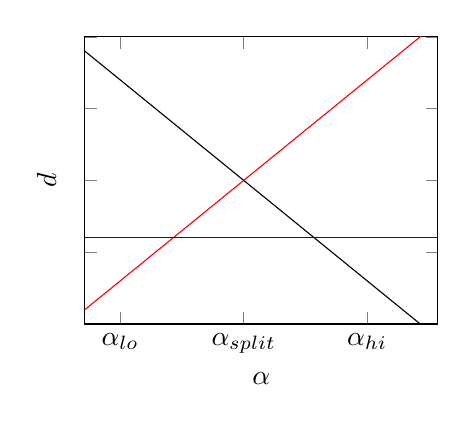
\begin{tikzpicture}
        \begin{axis}[ 
        xlabel=$\alpha$,
        ylabel={$d$},
        xmin=0.4,
        xmax=0.9,
        xtick={0.45,0.625,0.8},
        xticklabels={$\alpha_{lo}$, $\alpha_{split}$, $\alpha_{hi}$},
        width=0.5\textwidth,
        yticklabels={,,}
        ] 
        \addplot[mark=none, red] {-3+8*x}; 
        \addplot[mark=none, black] {-8*x+7};
        \addplot[mark=none, blue] {1.2};
        \end{axis} 
    \end{tikzpicture}
    \caption{Simply calculating the split values between the start and the end value of the range $[\alpha_{lo}, \alpha_{hi}]$ will not necessarily lead to the optimal values. By doing so, the blue line (constant $d$ value) will not be considered.}
    \label{fig:notoptimal}
\end{figure}

In order to solve this, we can recursively check each resulting interval again if it contains different merging behaviors.

\begin{figure}[h]
    \centering
    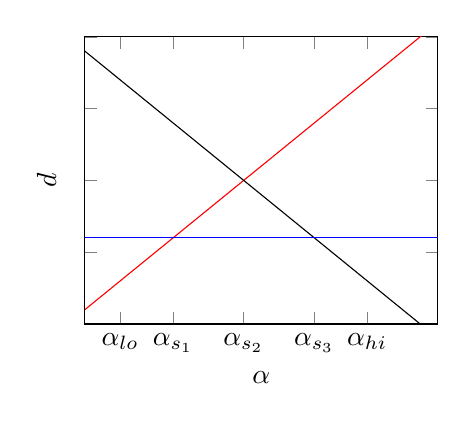
\begin{tikzpicture}
        \begin{axis}[ 
        xlabel=$\alpha$,
        ylabel={$d$},
        xmin=0.4,
        xmax=0.9,
        xtick={0.45,0.525,0.625,0.725,0.8},
        xticklabels={$\alpha_{lo}$, $\alpha_{s_1}$, $\alpha_{s_2}$, $\alpha_{s_3}$, $\alpha_{hi}$},
        width=0.5\textwidth,
        yticklabels={,,}
        ] 
        \addplot[mark=none, red] {-3+8*x}; 
        \addplot[mark=none, black] {-8*x+7};
        \addplot[mark=none, blue] {1.2};
        \end{axis} 
    \end{tikzpicture}
    \caption{Simply calculating the split values between the start and the end value of the range $[\alpha_{lo}, \alpha_{hi}]$ will not necessarily lead to the optimal values. By doing so, the blue line (constant $d$ value) will not be considered.}
    \label{fig:notoptimal2}
\end{figure}

By calculating the split points recursively, the example in figure \ref{fig:notoptimal2} will result in the intervals $[\alpha_{lo}, \alpha_{s_1}]$, $[\alpha_{s_1}, \alpha_{s_2}]$, $[\alpha_{s_2}, \alpha_{s_3}]$ and $[\alpha_{s_3}, \alpha_{s_{hi}}]$. The optimal distance between $\alpha_{s_1}$ and $\alpha_{s_3}$ is covered now, but the results contain one unncessary interval as $\alpha_{s_2}$ still splits two intervals. The algorithm can check if older splits are still relevant, however the runtime cost to do so will be more expensive than carrying one additional interval with the same distance. We can use this knowledge and adapt algorithm \ref{alg:alphalinkage1}.

\begin{algorithm}[H]
    \KwData{input data $p_1, ..., p_N$, initial states $st$}
    \KwResult{$k$ intervals $[\alpha_0, \alpha_1], ..., [\alpha_{k-1},\alpha_k]$}
    \For{$iteration\gets1$ \KwTo $N-1$}{
        \ForEach{state $s \in st$}{%
        remove state $s$\;
        ranges $\gets$ find ranges between $s.\alpha_{lo}$ and $s.\alpha_{hi}$\;
        \ForEach{range $r \in ranges$}{%
                $cand \gets$ candidate for range\;
                $ms \gets$ merge $cand$\;
                add state $ms$ with range $r$ to the end of $st$\;
        }
      }
    }
    \caption{By calculating the split points between $\alpha_{lo}$ and $\alpha_{hi}$ recursively, we ensure that no optimal interval is left out.}
    \label{alg:alphalinkage2}
\end{algorithm}

As experimental results turn out to need a lot of memory (up to $\approx$ 20 GB for 300 points and 20,000 states), we want to adapt algorithm \ref{alg:alphalinkage2} so that it uses less memory. The memory usage scales relative to the amount of currently in-memory stored states, so the goal is to reduce these. As the amount of states is much larger than the amound of iterations, we calculate and evaluate the leave nodes of the tree and keep the alternative merges stored. This results in algorithm \ref{alg:alphalinkage3}.

\begin{algorithm}[H]
    \KwData{input data $p_1, ..., p_N$, initial states $st$}
    \KwResult{$k$ intervals $[\alpha_0, \alpha_1], ..., [\alpha_{k-1},\alpha_k]$}
    \While{$\|st\| > 0$}{
        \ForEach{state $s \in st$}{%
        remove state $s$\;
        \eIf{$s$ is final}{
          evaluate $s$\;
          }{
          ranges $\gets$ find ranges between $s.\alpha_{lo}$ and $s.\alpha_{hi}$\;
            \ForEach{range $r \in ranges$}{%
                    $cand \gets$ candidate for range\;
                    $ms \gets$ merge $cand$\;
                    add state $ms$ with range $r$ to the beginning of $st$\;
            }
         }
      }
    }
    \caption{Instead of calculating the nodes layerwise, this algorithm works pathwise, i.e. it goes down one path of a tree to a leaf node and evaluates it before continuing with the next split. This approach needs much less memory than the previous algorithms and has about the same runtime as shown in figure \ref{fig:performance}.}
    \label{alg:alphalinkage3}
\end{algorithm}

\begin{figure}[h]
\centering
\begin{minipage}{.45\textwidth}
  \centering
  \includegraphics[width=\linewidth]{images/memory_mnist_ac}
\end{minipage}\hfill
\begin{minipage}{.45\textwidth}
  \centering
  \includegraphics[width=\linewidth]{images/runtime_mnist_ac}
\end{minipage}
\caption{The depth first implementation needs less memory and also has a better runtime compared to the breadth first implementation.}
\label{fig:performance}
\end{figure}

Instead of merging iteratively and steadily shrinking the intervals, we propose an algorithm with a geometric motivation. We are again evaluating an interval $[\alpha_{lo}, \alpha_{hi}]$, but we interprete the different merges as linear functions depending on $\alpha$. We can start by calculating the merge candidate for the start value $\alpha_{lo}$ and calculate the next intersection that will yield to the next merge. By calculating all the intersections of linear functions, we can also determine all the different intervals for the range $[\alpha_{lo}, \alpha_{hi}]$, where different merging behaviors occure. Algorithm \ref{alg:alphalinkage4} describes this procedure.

\begin{algorithm}[H]
    \KwData{input data $p_1, ..., p_N$, start value $\alpha_{lo}$, end value $\alpha_{hi}$}
    \KwResult{$k$ intervals $[\alpha_0, \alpha_1], ..., [\alpha_{k-1},\alpha_k]$}
    $\alpha \gets \alpha_{lo}$\;
    linear function $lf \gets$ get lf for alpha\;
    \While{$\alpha < \alpha_{hi}$}{
        $\alpha_{new} \gets$ calculate next split for $\alpha$\; 
        $lf \gets$ get lf for $\alpha_{new}$\;
        $\alpha \gets \alpha_{new}$
    }
    \caption{}
    \label{alg:alphalinkage4}
\end{algorithm}

\begin{figure}[h]
    \centering
    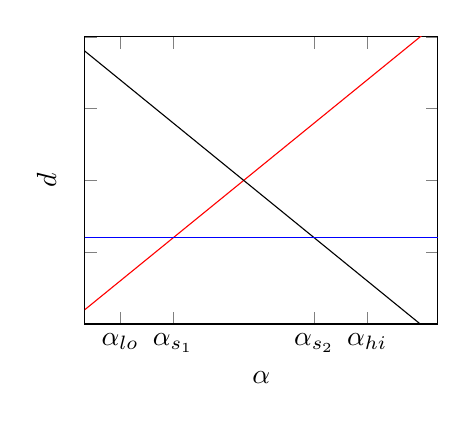
\begin{tikzpicture}
        \begin{axis}[ 
        xlabel=$\alpha$,
        ylabel={$d$},
        xmin=0.4,
        xmax=0.9,
        xtick={0.45,0.525,0.725,0.8},
        xticklabels={$\alpha_{lo}$, $\alpha_{s_1}$, $\alpha_{s_2}$, $\alpha_{hi}$},
        width=0.5\textwidth,
        yticklabels={,,}
        ] 
        \addplot[mark=none, red] {-3+8*x}; 
        \addplot[mark=none, black] {-8*x+7};
        \addplot[mark=none, blue] {1.2};
        \end{axis} 
    \end{tikzpicture}
    \caption{Simply calculating the split values between the start and the end value of the range $[\alpha_{lo}, \alpha_{hi}]$ will not necessarily lead to the optimal values. By doing so, the blue line (constant $d$ value) will not be considered.}
    \label{fig:optimal}
\end{figure}

\section{Performance Optimizations}

In order to have real-world applications, the proposed algorithms should run in an efficient way, i.e. it should not take the $\alpha$-linkage algorithms too much time to run. A first python implementation took days to run, but switching to C++ and using its advantages took down the runtime to hours. However, there are more optimization methods that we used in order to improve the runtime.

\subsection{Dynamic Programming}

One of the most time-consuming parts was the calculating of the distances. For each pair of clusters $C_i, C,j$ the distance had to be calculated for each clustering state. We optimized this by using dynamic programming and stored the distance matrices $D_{lower}$ and $D_{upper}$ for each state. The naming results from the different interpolation settings where we interpolate from one linkage distance (lower) to another linkage distance (upper), e.g. the setting in equation \ref{eq:singlecomplete} describes the interpolation from single linkage (lower) to complete linkage (upper). In this example we then store the pairwise distances for both single linkage and complete linkage and in order to find the merge candidates we have to do iterate over the distance matrices instead of calculating the distances over and over again. When we merge two clusters, we then update the distance matrices for the given state. Table \ref{dp:distances} shows an example for the pairwise distances of clusters $i$ and $j$.

\begin{table}[h]
    \centering
    \begin{tabular}{|l | l l l l l|}
    \hline
    j\textbackslash i & 0 & 1 & 2 & 3 & 4\\ \hline
    0 & 0 & 1.243 & 1.512 & 2.468 & 5.1243\\
    1 & 1.243 & 0 & 2.443 & 3.1412 & 4.443\\
    2 & 1.512 & 2.443 & 0 & 3.8988 & 6.827\\
    3 & 2.468 & 3.1412 & 3.8988 & 0 & 5.72\\
    4 & 5.1243 & 4.443 & 6.827 & 5.72 & 0\\ \hline
    \end{tabular}
    \caption{Storing the pairwise distances of all clusters avoids calculating the distances over and over again.}
    \label{dp:distances}
\end{table}

One observation that we can make is that the matrix has a lot of redundant values, because $D(i,j) = D(j,i)$. Removing these rendundant values will result in a trade-off between copying and indexing costs and will be discussed in the following section. Another optimization we can do is storing the indices of the active clusters, i.e. the clusters that can get merged. Once two clusters got merged, they cannot be merged any further, only the resulting cluster can. So we then do not have to consider the old clusters anymore and can remove them from the set of active indicies. This allows us to find the merge candidates faster as the pool of candidates gets smaller.

\subsection{Trade-Off between Copying and Indexing Costs}

Currently we can access the costs for a pair of clusters $C_i$ and $C_j$ through $D[i,j]$ or $D[i + j * width]$ for flattened matrices. These indices are very easy to calculate. In order to remove the redundant values from the distance matrix we remove all values below the diagonal as shown in table \ref{dp:distances2}.

\begin{table}[h]
    \centering
    \begin{tabular}{|l | l l l l l|}
    \hline
    j\textbackslash i & 0 & 1 & 2 & 3 & 4\\ \hline
    0 & 0 & 1.243 & 1.512 & 2.468 & 5.1243\\
    1 & & 0 & 2.443 & 3.1412 & 4.443\\
    2 & & & 0 & 3.8988 & 6.827\\
    3 & & & & 0 & 5.72\\
    4 & & & & & 0\\ \hline
    \end{tabular}
    \caption{Storing the pairwise distances of all clusters avoids calculating the distances over and over again.}
    \label{dp:distances2}
\end{table}

In addition to that we can also remove the diagonal values as they represent the distances between the same clusters and are thus always zero. This results in table \ref{dp:distances3}.

\begin{table}[h]
    \centering
    \begin{tabular}{|l | l l l l l|}
    \hline
    j\textbackslash i & 0 & 1 & 2 & 3 & 4\\ \hline
    0 & & 1.243 & 1.512 & 2.468 & 5.1243\\
    1 & & & 2.443 & 3.1412 & 4.443\\
    2 & & & & 3.8988 & 6.827\\
    3 & & & & & 5.72\\
    4 & & & & &\\ \hline
    \end{tabular}
    \caption{Storing the pairwise distances of all clusters avoids calculating the distances over and over again.}
    \label{dp:distances3}
\end{table}

The matrices are now smaller, so they need less memory. In the example, we changed a matrix of the size $25$ to a matrix of the size $10$. In general a matrix of the size $n$x$n$ will be compressed to a matrix of the size $\frac{n^2-n}{2}$. The lower amount of needed memory also results in less copying costs that will lead to a better runtime. However, the indexing is not as easy anymore. For easier storage, we again work with flattened matrices, the indexing for the resulting list is shown in equation \ref{eq:indexing}.

\begin{equation}
    \begin{aligned}
        index(i,j) = \frac{width * (width - 1)}{2} - \frac{(width - j) * (width - j - 1)}{2} + i - j - 1
    \end{aligned}
    \label{eq:indexing}
\end{equation}

Calculating this index in a nested loop is very expensive, however we calculate the part that does not depend on $i$ in the outer loop and thus only need to add $i$ in the inner loop. This does not only yield to a lower memory usage of $\approx 30\%$, but also increases the runtime by TODO.

\subsection{Implementation-specific Optimizations}

In order to optimize the implementation even further, we will have a look into the implementation. One optimization that already was briefly described is the flatterning of the matrices, so the resulting list will be one-dimensional and can be iterated easier and faster.

Another observation is that copy operations are computationally expensive, so we avoid them as much as possible. In the described algorithms (\ref{alg:alphalinkage1}, \ref{alg:alphalinkage2} and \ref{alg:alphalinkage3}) we removed a state from the list of states and added other states. In an optimized way, we do not remove the state and just overwrite the state with the resulting state. Once there are splits in the current interval, the state gets overwritten and additional states get added to the list.

We can also optimize the way of updating the distance matrices. Instead of adding new clusters there for a merge of clusters $i$ and $j$ we update the distances of $i$ to all active clusters with the distances of the resulting cluster. The distances of the cluster $j$ will not be considered for merges anymore as the index $j$ gets removed from the active indices. This has the advantage that the size of the distance matrices will not increase after merges.

Also, the data types make an important contribution to the memory usage. Instead of using double precision floating point values, single precision is enough to clearly identify and separate all the resulting intervals. Same goes for the distances as we only need the minimum and maximum distances, that are not effected by loss of precision. To store the indices of the clusters, we know that they will not exceed $2^{16}$, so they can be store as half precision values.

\chapter{Optimizing the Metric}
\label{sec:beta}

In a similar fashion as described in section \ref{chapter:alphalinkage} this sections aims to optimize a metric that is a linear combination of several metrics. For instance, images can have a 2D pixel representation and a text describing the each image. Combining these features for clustering tasks can be problematic as it is not how the optimal weight between these features should be. Does a word describe more than a subset of the image, are the features equally important or does the pixel image lead to better clusterings? With $\beta$-linkage we provide a framework based on $\alpha$-linkage that calculates different merges based on linear combinations of representations and leads to optimized clusterings.

\begin{figure}[h]
    \centering
    \includegraphics[width=0.7\textwidth]{images/ExampleDataset}
    \caption{Combining several metrics seems often natural and can lead to improved results as in this example where we project a dataset on both axes.}
    \label{fig:metrics}
\end{figure}

For instance, figure \ref{fig:metrics} shows a set of points that might be put in clusters easily. However, if you only look at the distance regarding the $X_1$-axis or the $X_2$-axis clustering will be very difficult, because each of the axis does not describe the spatial correlation anymore. This example is selected on purpose to motivate the following experiments where we learn optimal combinations of different metrics.\\ 

To interpolate between $d_0$ and $d_1$, we use the same interpolation as discussed in section \ref{chapter:alphalinkage}. We use a parameter $\beta \in [0,1]$ and weight the metrics as shown in equation \ref{eq:betalinkage}.

\begin{equation}
d_\beta(x,x') = (1 - \beta) \cdot d_0(x,x') + \beta \cdot d_1(x,x')
\label{eq:betalinkage}
\end{equation}

\begin{equation}
d_\beta(x,x') = d_0(x,x') + \beta \cdot (d_1(x,x') - d_0(x,x'))
\label{eq:betalinear}
\end{equation}

We can then compete all possible discontinuities by comparing the distances of given clusters $(x, x')$ and $(y, y')$. As $d_\beta(x,x')$ is a linear function depending on $\beta$ (see equation \ref{eq:betalinear}), we can compute all discontinuities by solving the following equation.

\begin{align*}
&d_\beta(x,x') = d_\beta(y,y')\\
&(1 - \beta) \cdot d_0(x,x') + \beta \cdot d_1(x,x') = (1 - \beta) \cdot d_0(y,y') + \beta \cdot d_1(y,y')\\
&d_0(x,x') - \beta \cdot d_0(x,x')  + \beta \cdot d_1(x,x') = d_0(y,y') - \beta \cdot d_0(y,y') + \beta \cdot d_1(y,y')\\
&\beta \cdot (- d_0(x,x') + d_1(x,x') + d_0(y,y') - d_1(y,y')) = - d_0(x,x') + d_0(y,y')\\
&\beta = \frac{- d_0(x,x') + d_0(y,y')}{- d_0(x,x') + d_1(x,x') + d_0(y,y') - d_1(y,y')}
\label{eq:discont}
\end{align*}

As we know that the function $d_\beta$ is a linear function depending on $\beta$ and we showed that all discontinuities depend on four points, we know that there at most $O(n^4)$ well-defined intervals $I_i \in [0,1]$ for any clustering instance $S$, i.e. in any interval $I_i$ the algorithm will merge the same two points.

\todo[inline]{more details / explanations}

% \chapter{$\alpha$-$\beta$-Linkage}

\section{Bilinear Interpolation between three different linkage strategies}

\section{Adapted Algorithm}

\chapter{Experimental Setup}
\label{chapter:setup}

This work evaluates the proposed algorithms for image and text data. This chapter describes the used datasets and evaluation methods.

\section{Data Sets}
\label{chapter:datasets}

\subsection{Synthetic Data}

To motivate our approach, we manually created a dataset containing disks and rings as shown in figure \ref{fig:disksrings}. In this case, we know that single linkage performs well clustering the two rings, however it might be problematic to cluster the disks. On the other hand, complete linkage is expected to cluster the disks very well, but it might connect the two rings earlier than wanted. This data motivates our approach of interpolating between different linkage strategies, however the data is not natural and real-world datasets are very likely to have a different structure. 

\begin{figure}[h]
    \centering
    \includegraphics[width=0.7\textwidth]{images/RingsDisks}
    \caption{We use disks and rings as a sample dataset to motivate our $\alpha$-linkage approach. The dataset contains four clusters, two disks and two rings.}
    \label{fig:disksrings}
\end{figure}

\subsection{Text Data}

\paragraph{Never-Ending Language Learner data.} The Never-Ending Language Learner (NELL) is a learning agent that reads the web, extracts data and verifies beliefs \cite{Mitchell:2015:NL:2886521.2886641, Mitchell:2018:NL:3210350.3191513}. NELL, for example, knows that "Pittsburgh" is located in "Pennsylvania". These beliefs represent different noun-phrases such as "Pittsburgh" and "Pennsylvania". The noun-phrases belong to certain categories, e.g.``Pittsburg'' is a ``City'' and ``Pennsylvania'' is a ``State''. These subcategories both belong to the main category "Geopolitical Location". Figure \ref{fig:nell_beliefs} shows such a knowledge graph. While there are already different subcategories, the goal for a hierarchical clustering algorithm here could be to extract new useful subcategories.

\begin{figure}[h]
    \centering
    \includegraphics[width=0.7\textwidth]{images/nell_beliefs}
    \caption{The Never-Ending Language Learner represents different entities and their correlations \cite{Mitchell:2018:NL:3210350.3191513}.}
    \label{fig:nell_beliefs}
\end{figure}

The used dataset, extracted web-information by NELL, contains 32 different main categories, such as "Animal", "Location" or "Person". We limit each of these categories up to 250 and 1000 different entities that belong to different subcategories, so we can run experiments with 250 points and later on with 1000 points. Exemplary entities for the category "Animal" are "Otter", "Squirrel" or "Wolf". 
\newpage
\subsection{Image Data}

\paragraph{MNIST handwritten digits.} The MNIST handwritten digit database contains images of the handwritten digits from zero to nine \cite{lecun-mnisthandwrittendigit-2010}. Samples of these images are shown in figure \ref{fig:mnist}. Its training set contains a total of 60,000 images, where each image is represented as a 784-dimensional vector corresponding to an image with $28 \times 28$ black and white pixels.

\begin{figure}[h]
    \centering
    \includegraphics[width=0.7\textwidth]{images/mnist}
    \caption{The MNIST handwritten digits database contains 60,000 black and white images of handwritten digits ranging from zero to nine. These samples show ten randomly drawn samples for each label represented as a $28 \times 28$ pixel image \cite{lecun-mnisthandwrittendigit-2010}.}
    \label{fig:mnist}
\end{figure}

The goal of clustering MNIST images is to find an unsupervised learning method that can distinguish between black and white images. In addition, we can define various clustering tasks where we pick a subsample of the ten labels and then try to transfer the results to other subsamples. For example, we first cluster images labeled as zero, one, two, three or four and later apply the gained knowledge for clustering images labeled as five, six, seven, eight or nine. These types of experiments allow high-level transfer learning if we define several different clustering tasks, e.g. for five different labels there are $10 \choose 5$ $= 252$ different combinations of labels.\\

Another observation that results from hierarchical clustering is the similarity of different labels, i.e. which labels are likely to get clustered together. For instance, we would expect images of characters 6 and 9, 3 and 8 or 2 and 5 to have some attributes in common and thus get clustered together rather than with other digits.

\paragraph{CIFAR-10.} Another image dataset this thesis uses for evaluation is the CIFAR-10 dataset that contains 60,000 RGB images of ten different categories \cite{Krizhevsky2009LearningML}. Each image consists of $32 \times 32$ pixels and is thus represented as a 3072-dimensional vector ($32 \times 32 \times 3$). The categories and ten random images from each are shown in figure \ref{fig:cifar10}.

\begin{figure}[h]
    \centering
    \includegraphics[width=0.7\textwidth]{images/cifar10}
    \caption{The CIFAR-10 database contains 60,000 RGB images of the ten shown different classes. These samples show ten randomly drawn samples for each label represented as a $32 \times 32$ pixel image \cite{Krizhevsky2009LearningML}.}
    \label{fig:cifar10}
\end{figure}

As the amount of images and the amount of classes is equal to the ones in the MNIST dataset, we can also try similar experiments. The main difference is that the images consist of RGB pixels instead of black and white pixel values.

\paragraph{CIFAR-100.} The CIFAR-100 dataset contains similar images, but instead of 6,000 images each for 10 classes, it consists of 600 images for each of 100 classes. The classes are divided into 20 superclasses each containing five subclasses. Examples of superclasses and corresponding subclasses are shown in table \ref{table:cifar100data}. 

\begin{table}[h]
    \centering
    \begin{tabular}{|l|l|}
    \hline
    superclass      & subclasses                                  \\ \hline
    aquatic mammals & beaver, dolphin, otter, seal, whale         \\
    fish            & aquarium fish, flatfish, ray, shark, trout  \\
    flowers         & orchids, poppies, roses, sunflowers, tulips \\
    people          & baby, boy, girl, man, woman                 \\ 
    reptiles        & crocodile, dinosaur, lizard, snake, turtle  \\ \hline               
    \end{tabular}
    \caption{The CIFAR-100 dataset contains 20 different superclasses, each with five different subclasses leading to 100 classes overall. The images are represented in the same way as in the CIFAR-10 dataset, i.e. by a 3072-dimensional vector \cite{Krizhevsky2009LearningML}.}
    \label{table:cifar100data}
\end{table}

Having superclasses and subclasses allows clustering between different subclasses within a superclass and also between different superclasses. This allows more experiments than for the CIFAR10 data.

\paragraph{Omniglot.}The Omniglot dataset contains 1623 handwritten characters from 30 different alphabets, where each character is represented by 20 different images. Each image is black and white and represented by $105 \times 105$ pixels \cite{Lake1332}. Figure \ref{fig:omniglotcharacters} shows characters of the more well-known Latin, Greek and Hebrew alphabets that are included in the dataset together with less known alphabets such as Tagalog, a language spoken as a first language by 25\% of the population of the Philippines.

\begin{figure}[h]
\centering
\begin{minipage}{.32\textwidth}
  \centering
  \includegraphics[width=\linewidth]{images/latin}
\end{minipage}
\begin{minipage}{.32\textwidth}
  \centering
  \includegraphics[width=\linewidth]{images/greek}
\end{minipage}
\begin{minipage}{.32\textwidth}
  \centering
  \includegraphics[width=\linewidth]{images/hebrew}
\end{minipage}
\caption{The Omniglot dataset contains handwritten characters of different alphabets, such as Latin (left), Greek (middle) and Hebrew (right) \cite{Lake1332}.}
\label{fig:omniglotcharacters}
\end{figure}

The Omniglot dataset is similar to the MNIST dataset as it also contains handwritten characters, however it has more different characters and fewer images for each of the characters. This allows us to run more learning tasks. In addition, the dataset also contains stroke data of each of the images, i.e.\ the time series data of the actual drawings where each observation corresponds to a (x,y)-coordinate together with a timestamp. This gives us insight into the order in which the character was written. Figure \ref{fig:omniglotstroke} shows an example of strokes for one character of the Tagalog alphabet.

\begin{figure}[h]
  \centering
  \includegraphics[width=.6\textwidth]{plots/demo_strokes}
  \caption{The stroke data gives a time series representation of the Omniglot drawings that indicate in which order the characters were written \cite{Lake1332}.}
  \label{fig:omniglotstroke}
\end{figure}

\section{Pruning}

In order to evaluate a cluster tree together with the target labels, we have to prune the tree into the corresponding number of $k$ target clusters, i.e.\ the $k$ different classes of the target data. Therefore, we evaluate the costs of all possible combinations of $k$ clusters and select the best clusters. Figure \ref{fig:pruning} shows an example of how we can prune a cluster tree into $k = 3$ clusters by either using the clusters $C, D$ and $E$ or the clusters $B, F$ and $G$.

\begin{figure}[h]
\centering
\begin{minipage}{.45\textwidth}
  \centering
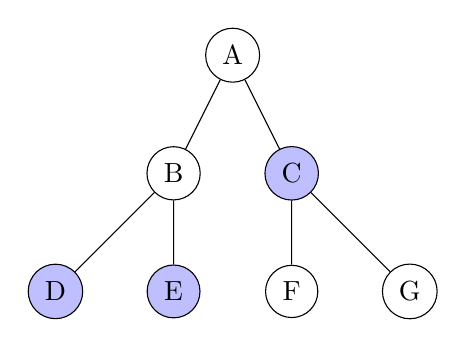
\begin{tikzpicture}
 
\node[circle,draw]{A}
	child { node[circle,draw] {B}
    child { node[circle,draw,fill=blue, fill opacity=0.25,text opacity=1] {D}}
	  child { node[circle,draw,fill=blue, fill opacity=0.25,text opacity=1] {E}}
    child[missing]{}
  }
	child { node[circle,draw,fill=blue, fill opacity=0.25,text opacity=1] {C}
    child[missing]{}
    child { node[circle,draw] {F}}
	  child { node[circle,draw] {G}}
  }
;
\end{tikzpicture}
\end{minipage}
\begin{minipage}{.45\textwidth}
  \centering
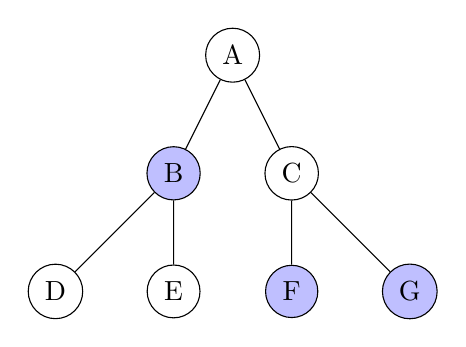
\begin{tikzpicture}
 
\node[circle,draw]{A}
	child { node[circle,draw,fill=blue, fill opacity=0.25,text opacity=1] {B}
    child { node[circle,draw] {D}}
	  child { node[circle,draw] {E}}
    child[missing]{}
  }
	child { node[circle,draw] {C}
    child[missing]{}
    child { node[circle,draw,fill=blue, fill opacity=0.25,text opacity=1] {F}}
	  child { node[circle,draw,fill=blue, fill opacity=0.25,text opacity=1] {G}}
  }
;
\end{tikzpicture}
\end{minipage}
\caption{There are multiple ways we can prune a cluster tree into $k$ clusters.}
\label{fig:pruning}
\end{figure}

However, we still have to find a way to calculate the preferred pruning of a cluster tree into $k$ clusters, i.e.\ whether in case of figure \ref{fig:pruning} we would prefer the pruning on the left or the one on the right.

\section{Cost functions}
\label{chapter:costfunctions}

In order to evaluate the quality of a clustering, we need some kind of cost function that compares the generated clustering $C_1,...,C_k$ with the target clustering $C_1^*, ..., C_k^*$ and calculates a quality score indicating how good they match. 

\paragraph{Majority Cost.} One method to compare them is the Majority distance as shown in equation \ref{eq:majoritydistance} where $n$ is the number of sampled points.

\begin{equation}
    \begin{aligned}
        cost_{Majority}(C_{1:k}, C_{1:k}^*) = \frac{1}{n} \sum_{i=1}^k \min_{j \in [m]} |C_i - C'_j|
    \end{aligned}
    \label{eq:majoritydistance}
\end{equation}

This cost function is motivated by finding corresponding clusters with the lowest distance, i.e. each generated cluster gets matched with the optimal target cluster and the cost is the average difference between the matched cluster pairs. However, two generated clusters can be matched with the same target cluster. 

\paragraph{Hamming Cost.} This motivates the Hamming distance as shown in figure \ref{eq:hammingdistance}. We denote $\mathbb{S}_k$ as all possible permutations of the $k$ clusters.

\begin{equation}
    \begin{aligned}
        cost_{Hamming}(C_{1:k}, C'_{1:k}) = \frac{1}{n} \min_{\sigma \in \mathbb{S}_k} \sum_{i=1}^k |C_i - C'_{\sigma_i}|
    \end{aligned}
    \label{eq:hammingdistance}
\end{equation}

However, the Hamming distance contains an assignment problem to find the optimal matching $\sigma$ between the generated clusters and the target clusters. Table \ref{table:matching} shows how such a matching can look like.

\begin{table}[h]
    \centering
    \begin{tabular}{|l | l l l l l|}
    \hline
    j\textbackslash i & 1 & 2 & 3 & 4 & 5\\ \hline
    1 & 20 & \cellcolor{blue!25}15 & 30 & 50 & 40\\
    2 & 80 & 10 & \cellcolor{blue!25}15 & 20 & 30\\
    3 & \cellcolor{blue!25}20 & 30 & 50 & 80 & 60\\
    4 & 30 & 50 & 40 & \cellcolor{blue!25}20 & 10\\
    5 & 20 & 30 & 40 & 50 & \cellcolor{blue!25}25\\ \hline
    \end{tabular}
    \caption{In order to calculate the Hamming distance between two clusterings, we have to calculate the optimal mapping that results in the lowest distance for these two clusterings. For distances between clusterings $C_1^i, ..., C_k^i$ and $C_1^j, ..., C_k^j$ we can calculate the optimal mapping (highlighted cells) in a brute force way or more efficiently with the Hungarian method \cite{kuhn1955hungarian, munkres1957algorithms}.}
    \label{table:matching}
\end{table}

While solving the assignment with a brute force strategy would result in $O(n!)$ complexity, Harold Kuhn introduced the Hungarian method to solve the problem in $O(n^4)$ complexity \cite{kuhn1955hungarian}. Later on, James Munkres modified the algorithm to $O(n^3)$ complexity \cite{munkres1957algorithms}. In general, we can say that it  makes sense to use the Hungarian method when there are more than five target classes. A detailed explanation of the Hungarian method is included in Appendix \ref{sec:hungarian}.

\section{Parameter Advising}

Our settings average over multiple experiments and show one parameter $\alpha$ that represents the best clustering over all experiments, i.e. the algorithm automatically outputs the best result. For parameter advising, we select the top $k$ values of $\alpha$ for each experiment and calculate the clustering's cost with the best of the $k$ values of $\alpha$ \cite{deblasio2015parameter}. We select the pool of $\alpha$-values through the local optima for each of the $n$ experiments. The best $k$ values of $\alpha$, where $k << n$, can then be calculated with an integer optimization problem. A possible scenario where this setup is useful is by having a domain expert, who can select the best from $k$ suggested clusterings.\\

More formally, we want to to find the optimal parameters $\alpha_1^*, \dots, \alpha_k^*$ such that they optimize the utility $u$ of a clustering instance $S$ and the resulting cluster tree $T(S, \alpha)$ (see equation \ref{eq:advising}). In order to calculate the parameters $\alpha_1^*, \dots, \alpha_k^*$, we first have a look at parameter advising described as a facility location problem.

\begin{equation}
  \alpha_1^*, \dots, \alpha_k^*
  = \argmax_{\alpha_1, \dots, \alpha_k} \sum_{i=1}^N \max_{j \in [k]} u\bigl(S, T(S, \alpha_j)\bigr).
  \label{eq:advising}
\end{equation}

\paragraph{Facility Location Advising.} We create an integer optimization problem for a candidate set $\alpha_1, \dots, \alpha_m$ over the clustering instances $S_1, \dots, S_N$ and introduce the selection parameters $y_1, \dots, y_m \in \{0, 1\}$ that indicate whether $\alpha_j$ is used as one of the $k$ parameters. Also, we denote $x_{ij} \in \{0, 1\}$ as the auxiliary variable with the interpretation that $x_{ij} = 1$ whenever $\alpha_j$ is the best chosen parameter for problem instance $S_i$. This leads to the following optimization problem that maximizes the overall utility.

\begin{align*}
  \argmax_{x_{ij}, y_j} \qquad&\sum_{i = 1}^N \sum_{j = 1}^m x_{ij} u(S_i, T(S_i, \alpha_j)) \\
  \text{subject to} \qquad& \sum_{j=1}^m y_j = k \\
  & \text{for each $i \in [N]$, } \sum_{j=1}^m x_{ij} = 1 \\
  & \text{for each $i \in [N], j \in [M]$, } x_{ij} \leq y_j.
\end{align*}

Note that the optimization problem contains three constraints. $\sum_{j=1}^m y_j = k$ makes sure that exactly $k$ values are used, the second guarantees that we assign any clustering instance to at most one parameter, and the final constraint ensures that we only assign clustering instances to selected parameters. In our experiments, we use IBM ILOG CPLEX to solve these integer programming problems. However, the computation of the optimal values is very complex, so we also implement a greedy strategy that calculates approximately optimal values more efficiently.

\paragraph{Greedy Parameter Advising.} In a convex space, an optimal value $\alpha_n^*$ will also be optimal when calculating $k = n + 1$ optimal values. Leveraging this knowledge, we can iteratively calculate the optimal values $\alpha_1, \dots, \alpha_m$ step by step, where we first calculate $\alpha_1^*$ that has the largest utility over all clustering instances $S$ and then calculate $\alpha_2^*$ that results in the highest utility combined with $\alpha_1^*$ (see equation \ref{eq:greedypa}).

\begin{equation}
\sum_{i=1}^N \max\{u(S_i, T(S_i, \alpha_1)), u(S_i, T(S_i, \alpha_2)\} 
\label{eq:greedypa}
\end{equation}

The results of the experiments with the mentioned datasets are discussed in the following section \ref{sec:results}. % Experimental Setup

\chapter{Results and Discussion}
\label{sec:results}

We evaluated the in chapter \ref{chapter:alphalinkage} proposed algorithms with the in chapter \ref{chapter:datasets} discussed datasets aiming to find new subcategories for the text data and to generate better clusterings overall. The quality of the clusterings was calculated with the in chapter \ref{chapter:costfunctions} explained cost functions.

\section{Clustering Text Data}

We subsampled the NELL data to a maximum of 250 points in each class and then evaluated each of the 32 classes separately. Figure \ref{fig:nellresults} shows the resulting majority distances for the three different types of linear interpolation.

\begin{figure}[h]
\centering
\begin{minipage}{.3\textwidth}
  \centering
  \includegraphics[width=\linewidth]{images/nell_sc}
\end{minipage}
\begin{minipage}{.3\textwidth}
  \centering
  \includegraphics[width=\linewidth]{images/nell_sa}
\end{minipage}
\begin{minipage}{.3\textwidth}
  \centering
  \includegraphics[width=\linewidth]{images/nell_ac}
\end{minipage}
\caption{The omniglot dataset contains handwritten characters of different alphabets, such as Latin, Greek and Hebrew \cite{Lake1332}.}
\label{fig:nellresults}
\end{figure}

We observe that single linkage performs very poorly and complete linkage performs very well for the NELL data. Table \ref{table:nellresults} shows the improvements we got over the other clustering strategies.

\begin{table}[h]
    \centering
    \begin{tabular}{|l | l|}
    \hline
    Strategy & Majority Cost\\ \hline
    Single Linkage & 0.36871\\
    Average Linkage & 0.248913\\
    Complete Linkage & 0.15935\\
    $\alpha_{SC}(0.825)$ & 0.15442\\
    $\alpha_{AC}(0.825)$ & 0.15569\\\hline
    \end{tabular}
    \caption{Our proposed algorithm reduces the cost by $\Delta cost = 0.493\%$.}
    \label{table:nellresults}
\end{table}

The total improvement over the common linkage methods is $0.493\%$ and the best clustering we generated had an error of $15.442\%$. With this clustering we also managed to extract new subcategories as listed in table \ref{table:nellcategories}.

In addition to averaged costs, we also evaluated the clusterings for multiple values of $\alpha$. This is helpful in situations where a domain expert can select from multiple suggestions. For example, if we consider the best three values of $\alpha$, the domain expert can choose from three different clusterings. In order to calculate the $N$ best values of $\alpha$, we selected the 32 optimal values resulting from the experiments that led to an integer optimization problem. This resulted in ?????.

As our only formal guarantee was that there will be a maximum of $O(n^8)$ intervals in the range between single and complete linkage, we also had a look at the actual results. Since the proof for single and complete linkage in Balcan et. al \cite{DBLP:journals/corr/BalcanNVW16} relies on the fact that the distance $d_{SC}(X,Y,\alpha)$ is based on four points and a split between two merges thus is based on eight points, we would expect experiments containing average linkage to have more intervals, because the average linkage distance is based on all points of the clusters. Finding formal guarantees for the average distance is not a part of this thesis and will briefly be discussed in section \ref{section:futurework}.

\section{Clustering Image Data}

We first clustered the MNIST data. First experiments were run with 250 points in each run.

\begin{figure}[h]
\centering
\begin{minipage}{.3\textwidth}
  \centering
  \includegraphics[width=\linewidth]{images/MNIST_SC_250}
\end{minipage}
\begin{minipage}{.3\textwidth}
  \centering
  \includegraphics[width=\linewidth]{images/MNIST_SA_250}
\end{minipage}
\begin{minipage}{.3\textwidth}
  \centering
  \includegraphics[width=\linewidth]{images/MNIST_AC_250}
\end{minipage}
\caption{The omniglot dataset contains handwritten characters of different alphabets, such as Latin, Greek and Hebrew \cite{Lake1332}.}
\label{fig:mnist250}
\end{figure}

Figure \ref{fig:mnist250} shows the experimental results averaged over all 252 $10 \choose 5$ experiments, i.e. all different combinations of five unique labels. Again, we observe that interpolating between single and average linkage does not give us good results. Table \ref{table:mnist250results} summarizes the results we obtain for these experiments.

\begin{table}[h]
    \centering
    \begin{tabular}{|l | l|}
    \hline
    Strategy & Hamming Cost\\ \hline
    Single Linkage & 0.782354\\
    Average Linkage & 0.634206\\
    Complete Linkage & 0.441931\\
    $\alpha_{SC}(0.861624,)$ & 0.420714\\
    $\alpha_{AC}(0.849407)$ & 0.416627\\\hline
    \end{tabular}
    \caption{Our proposed algorithm reduces the cost by $\Delta cost = 2.5304\%$.}
    \label{table:mnist250results}
\end{table}

Reducing the cost by $\Delta cost = 2.5304\%$ seems to be a good result already. However the goal was to learn a parameter $\alpha$ that represents the entire dataset well. Because the procedure is very ressource-expensive, the results only looked at the first 500 points of the dataset as we clustered points from five labels in experiments of 250 points, i.e. we were using the first 50 points for each of the ten labels. This led us to running the same setting with other batches of the dataset to see if the subset of 500 points gives a good representation of the entire dataset. Figure ??? shows the results for the second batch and unfortunately the curves look quite differently, i.e. the batch did not give a good representation for the dataset.

To overcome this problem, we decided to scale up the experiments, so each of them used 1,000 instead of 250 points. As we used cloud computing to run the experiments in a reasonable time, we only evaluated the single to complete linkage and the average to complete linkage interpolation. We started with the single to complete linkage interpolation, where we show the results for the first six batches in figure \ref{fig:mnist1000sc}. Each batch contains 2,000 points, i.e. the six batches cover the first 12,000 points of the dataset.

\begin{figure}[h]
\centering
\begin{minipage}{.3\textwidth}
  \centering
  \includegraphics[width=\linewidth]{images/mnist-sc-0}
\end{minipage}
\begin{minipage}{.3\textwidth}
  \centering
  \includegraphics[width=\linewidth]{images/mnist-sc-1}
\end{minipage}
\begin{minipage}{.3\textwidth}
  \centering
  \includegraphics[width=\linewidth]{images/mnist-sc-2}
\end{minipage}
\begin{minipage}{.3\textwidth}
  \centering
  \includegraphics[width=\linewidth]{images/mnist-sc-3}
\end{minipage}
\begin{minipage}{.3\textwidth}
  \centering
  \includegraphics[width=\linewidth]{images/mnist-sc-4}
\end{minipage}
\begin{minipage}{.3\textwidth}
  \centering
  \includegraphics[width=\linewidth]{images/mnist-sc-5}
\end{minipage}
\caption{The first six batches of the MNIST dataset result in similar curves when being evaluated between single and complete linkage.}
\label{fig:mnist1000sc}
\end{figure}

As the curves look quite similar, we also want to analyse if the optimal values are similar. Thus we calculate the hamming cost for the optimal value of $\alpha$ in table \ref{table:mnist1000sc}.

\begin{table}[h]
    \centering
    \begin{tabular}{|l | l l l l l l |}
    \hline
    Strategy & Batch 0 & Batch 1 & Batch 2 & Batch 3 & Batch 4 & Batch 5\\ \hline
    Single Linkage & 0.796901 & 0.797345 & 0.797171 & 0.797405 & 0.796766 & 0.797024\\
    Complete Linkage & 0.490468 & 0.461063 & 0.479825 & 0.475329 & 0.463321 & 0.487111\\
    $\alpha_{opt}$ & 0.87228 & 0.84419 & 0.778498 & 0.83199 & 0.82338 & 0.852251\\
    $cost_{opt}$ & 0.450012 & 0.416433 & 0.431143 & 0.423786 & 0.421103 & 0.446032\\
    $\Delta cost$ & 4.0456\% & 4.463\% & 4.8682\% & 5.1543\% & 4.2218\% & 4.1079\%\\\hline
    \end{tabular}
    \caption{Our proposed algorithm reduces the cost by up to $\Delta_{max} cost = 5.1543\%$.}
    \label{table:mnist1000sc}
\end{table}

We were running the same experiments for the interpolation between average and complete linkage.

\begin{figure}[h]
\centering
\begin{minipage}{.3\textwidth}
  \centering
  \includegraphics[width=\linewidth]{images/mnist-ac-0}
\end{minipage}
\begin{minipage}{.3\textwidth}
  \centering
  \includegraphics[width=\linewidth]{images/mnist-ac-1}
\end{minipage}
\begin{minipage}{.3\textwidth}
  \centering
  \includegraphics[width=\linewidth]{images/mnist-ac-2}
\end{minipage}
\begin{minipage}{.3\textwidth}
  \centering
  \includegraphics[width=\linewidth]{images/mnist-ac-3}
\end{minipage}
\begin{minipage}{.3\textwidth}
  \centering
  \includegraphics[width=\linewidth]{images/mnist-ac-4}
\end{minipage}
\begin{minipage}{.3\textwidth}
  \centering
  \includegraphics[width=\linewidth]{images/mnist-ac-5}
\end{minipage}
\caption{The omniglot dataset contains handwritten characters of different alphabets, such as Latin, Greek and Hebrew \cite{Lake1332}.}
\label{fig:mnist1000ac}
\end{figure}

\begin{table}[h]
    \centering
    \begin{tabular}{|l | l l l l l l |}
    \hline
    Strategy & Batch 0 & Batch 1 & Batch 2 & Batch 3 & Batch 4 & Batch 5\\ \hline
    Average Linkage & 0.664952 & 0.672583 & 0.623325 & 0.679929 & 0.657857 & 0.652774\\
    Complete Linkage & 0.490468 & 0.461063 & 0.479825 & 0.475329 & 0.463321 & 0.487111\\
    $\alpha_{opt}$ & 0.7869 & 0.7124 & 0.634 & 0.807697 & 0.536073 & 0.5305\\
    $cost_{opt}$ & 0.458167 & 0.406563 & 0.440964 & 0.451063 & 0.429849 & 0.431631\\
    $\Delta cost$ & 3.2301\% & 5.45\% & 3.8861\% & 2.4266\% & 3.3472\% & 5.548\%\\\hline
    \end{tabular}
    \caption{Our proposed algorithm reduces the cost by up to $\Delta_{max} cost = 5.548\%$.}
    \label{table:mnist1000ac}
\end{table}

The curves for interpolating between average and complete linkage in figure \ref{ref:mnist1000ac} vary more than the curves for interpolating between single and complete linkage \ref{fig:mnist1000sc}. This results in a higher variation in the optimal values of $\alpha$ and the performance increase as shown in table \ref{table:mnist1000ac}.

In order to compare the both interpolation strategies, we averaged over the six batches to to see how well the different batches fit to each other. The results are shown in figure \ref{fig:mnist1000avg}.

\begin{figure}[h]
\centering
\begin{minipage}{.45\textwidth}
  \centering
  \includegraphics[width=\linewidth]{images/mnist-sc-averaged}
\end{minipage}
\begin{minipage}{.45\textwidth}
  \centering
  \includegraphics[width=\linewidth]{images/mnist-ac-averaged}
\end{minipage}
\caption{Averaging the first six batches over both linkage strategies allows us to see how good they perform on the first 12,000 points of the MNIST dataset.}
\label{fig:mnist1000avg}
\end{figure}

Figure \ref{fig:mnist1000avg} shows that both strategies give a valuable improvement over single, average and complete linkage on the first 12,000 points of the MNIST dataset. The exact improvement is shown in table \ref{table:mnist1000avg}.

\begin{table}[h]
    \centering
    \begin{tabular}{|l | l |}
    \hline
    Strategy & Hamming Cost\\ \hline
    Single Linkage & 0.797102\\
    Average Linkage & 0.65857\\
    Complete Linkage & 0.476186\\
    $cost_{opt_{SC}}$ & 0.439207\\
    $\Delta cost_{SC}$ & 3.6979\%\\
    $cost_{opt_{AC}}$ & 0.443139\\
    $\Delta cost_{AC}$ & 3.3047\%\\\hline
    \end{tabular}
    \caption{Our proposed algorithm reduces the cost by up to $\Delta_{max} cost = 5.548\%$.}
    \label{table:mnist1000avg}
\end{table}

Table \ref{table:mnist1000avg} shows that the improvement for average to complete linkage interpolation is $3.3\%$ and for single to complete linkage it is $3.7\%$. The optimal cost corresponds to $\alpha = 0.856557$ in the $SC$ setting and $\alpha = 0.63275$ in the $AC$ setting.

\begin{figure}[h]
\centering
\begin{minipage}{.45\textwidth}
  \centering
  \includegraphics[width=\linewidth]{images/mnist-sc-random}
\end{minipage}
\begin{minipage}{.45\textwidth}
  \centering
  \includegraphics[width=\linewidth]{images/mnist-ac-random}
\end{minipage}
\caption{The first six batches of the MNIST dataset result in similar curves when being evaluated between single and complete linkage.}
\label{fig:mnist1000sc}
\end{figure}

\section{Parameter Advising} % Results and Discussion

\chapter{Conclusion}

In this work, we propose a data-driven solution to find the best algorithm, i.e.\ linkage strategy, for clustering tasks on a given dataset. In section \ref{chapter:alphalinkage} we introduce an algorithm to efficiently interpolate between the in section \ref{chapter:relatedwork} described linkage strategies. The final $\alpha$-linkage algorithm uses a sweep line approach to find the pairwise distance function that leads to merges with the lowest resulting cost, i.e.\ the optimal clusterings.\\

While the in section \ref{chapter:relatedwork} described approaches are less efficient, our approach is able to analyze large parts of the in section \ref{chapter:setup}  discussed real-world datasets using cloud computing. We summarize multiple key observations from the experiments in section \ref{sec:results}:
\begin{itemize}
\item Interpolating between single and complete linkage overcomes the hurdles of clustering data where both single and complete linkage perform better for some certain parts of the data. While single and complete linkage lead to an error of approximately $25\%$ for our synthetic data, in some experiments $\alpha$-linkage leads to optimal clusterings (i.e. an error of $0\%$).
\item For all our real-world datasets, we can sort the linkage strategies according to their quality in the following order (best first):
\begin{enumerate}
\item Complete Linkage
\item Average Linkage
\item Single Linkage
\end{enumerate}
\item Interpolating between single and average linkage does in general not lead to significant improvements.
\item When interpolating between single and complete or average and complete linkage, $\alpha$-linkage outperforms the used linkage strategies in all of our experiments with meaningful feature data.
\item Parameter Advising is a very powerful tool to provide more accurate clusterings. Our greedy implementation allows calculating the optimal parameters in an approximately optimal way very efficiently.
\end{itemize}

To be more precise, we show the results for the different datasets. In table \ref{table:comparison} we compare the single to complete linkage interpolation for all the discussed datasets\footnote{CIFAR-100 single to complete linkage was not discussed in this thesis.} in the batch setting. We notice that we achieve major improvements for all datasets and, excluding the synthetic data, receive similar values for $\alpha_{opt}$. This knowledge may be useful for transfer learning between different datasets in future work.

\begin{table}[H]
    \centering
    \begin{tabular}{|l | l | l | l | l | l |}
    \hline
    & Synthetic & NELL & MNIST & Omniglot & CIFAR-10\\ \hline
    $\alpha_{opt}$ & 0.169 & 0.918 & 0.857 & 0.908 & 0.917\\
    $\Delta_{cost}$ & 22.70\% & 1.20\% & 3.70\% & 1.0\% & 0.2\%\\\hline
    \end{tabular}
    \caption{Comparing the results over the different datasets while interpolating between single and complete linkage leads to similar parameters for many datasets.}
    \label{table:comparison}
\end{table}

Similar to table \ref{table:comparison}, we also show the results for interpolating between average and complete linkage in table \ref{table:comparison_ac}.

\begin{table}[H]
    \centering
    \begin{tabular}{|l | l | l | l | l | l | l |}
    \hline
    & Synthetic & NELL & MNIST & Omniglot & CIFAR-10 & CIFAR-100\\ \hline
    $\alpha_{opt}$ & 0.201 & 0.855 & 0.633 & 0.798 & 0.539 & 0.875\\
    $\Delta_{cost}$ & 0.29\% & 0.77\% & 3.30\% & 1.0\% & 0.83\% & 1.8\%\\\hline
    \end{tabular}
    \caption{Comparing the results over the different datasets while interpolating between average and complete linkage leads to a bigger spread of the parameters.}
    \label{table:comparison_ac}
\end{table}

In comparison to interpolating between single and complete linkage, we also obtain good improvements, however the optimal parameter $\alpha$ is spread more widely, i.e.\ it will be more difficult to reuse the gained knowledge for further use.\\

Also, we show in section \ref{sec:metric} that we can successfully apply the implemented framework to learning optimal metrics for given data as discussed in section \ref{sec:beta}. We achieve significant improvements by combining different data sources for the Omniglot data in different settings. Precisely, we improve the clusterings by up to $9\%$ when combining the stroke data distance with the cosine distance of the features extracted from a CNN that was trained on the MNIST data.

\paragraph{Future Work.} Nevertheless, we can think of further additions to this work. The trivial next step will be to combine metric learning with algorithm selection, as for now, we only evaluated the same setups independently, i.e.\ we used a static feature representation for algorithm selection and we used complete linkage for metric learning. At the point of writing this work, we are not exactly sure how difficult it will be to efficiently combine both aspects of this work, but we know that it is feasible and can be achieved in future work.\\

Also, after showing empirically that interpolating between average and complete linkage leads to fewer discontinuities and also fewer improvements than interpolating between single and complete linkage, we want to find a formal proof for it, so we know that interpolating between single and complete linkage will be more promising for the effective use of this framework.\\ 

The proposed algorithms only work for linear interpolation between two algorithms. In this setting, proving that in each interval we perform the same optimal merge is mostly trivial. As an adaption of our algorithms, we can think of interpolating between more algorithms, e.g.\ we could interpolate between single, average and complete linkage with a distance such as the following:

\begin{align*}
&\mathcal{D}_\text{SAC}(X,Y) = \alpha_1 \cdot \min\limits_{x \in X, y \in Y} d(x,y) + \alpha_2 \cdot \frac{1}{|X||Y|} \sum\limits_{x \in X, y \in Y} d(x,y) + (1-\alpha_1-\alpha_2) \cdot \max\limits_{x \in X, y \in Y} d(x,y)\\
&\text{s. t. } \{\alpha_1, \alpha_2\} \in [0,1] \text{ and } \alpha_1 + \alpha_2 \le 1
\end{align*}

However, the distance functions $d_{(\alpha_1, \alpha_2)}$ now are not linear anymore, as they depend on the two parameters $\alpha_1$ and $\alpha_2$. This means that our suggested sweep line approach will not work anymore, as the distance depending on the two parameter spans a two-dimensional space, where each split is a convex hull instead of a linear subspace. Figure \ref{fig:convexhull} shows the interval split depending on $\alpha$ on the left, and the split depending on $\alpha_1$ and $\alpha_2$ on the right. Moreover, it shows a very optimistic example where the splitting linear functions are parallel, however this might often not be the case, i.e.\ we will receive more different regions where it will be less intuitive to find the borders where one merge gets preferred over another (e.g.\ see figure \ref{fig:convexhulls2}).

\begin{figure}[h]
\centering
\begin{minipage}{.45\textwidth}
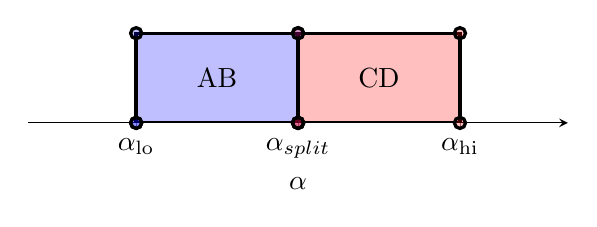
\begin{tikzpicture}
\begin{axis}[
    xmin=0, xmax=1,
    axis x line=bottom,% only show the bottom x axis
    xlabel={$\alpha$},
    xtick={0.2,0.5,0.8},
    xticklabels={$\alo$,$\alpha_{split}$,$\ahi$},
    hide y axis,    
    ymin=0,ymax=5,
    scatter/classes={%
        a={mark=o,draw=black}}
    ]

    \addplot [mark=*,very thick,fill=blue, fill opacity=0.25] coordinates {
        (0.2, 0)
        (0.2, 1)
        (0.5, 1)
        (0.5, 0)
        (0.2, 0)
    };
    \addplot [mark=*,very thick,fill=red, fill opacity=0.25] coordinates {
        (0.5, 0)
        (0.5, 1)
        (0.8, 1)
        (0.8, 0)
        (0.5, 0)
    };
    \node[] at (axis cs: 0.35,0.5) {AB};
    \node[] at (axis cs: 0.65,0.5) {CD};
\end{axis}
\end{tikzpicture}
\end{minipage}
\begin{minipage}{.45\textwidth}
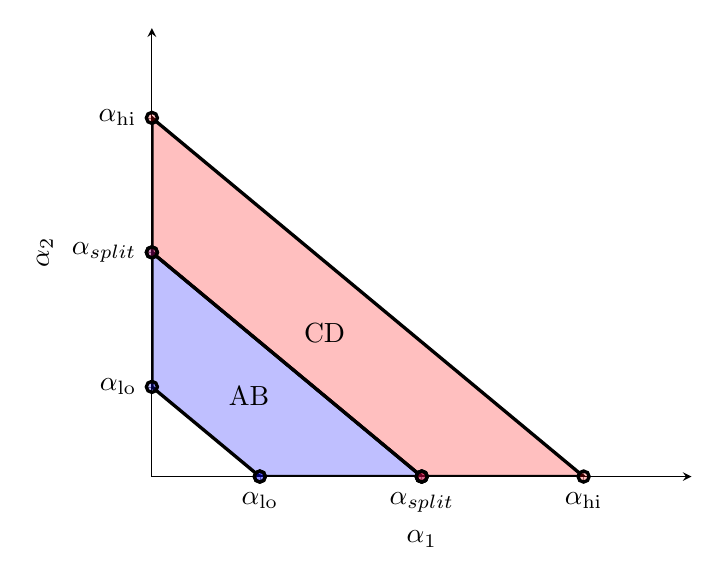
\begin{tikzpicture}
\begin{axis}[
    xmin=0, xmax=1,
    axis x line=bottom,% only show the bottom x axis
    axis y line=left,
    xlabel={$\alpha_1$},
    ylabel={$\alpha_2$},
    xtick={0.2,0.5,0.8},
    xticklabels={$\alo$,$\alpha_{split}$,$\ahi$},  
    ytick={0.2,0.5,0.8},
    yticklabels={$\alo$,$\alpha_{split}$,$\ahi$},  
    ymin=0,ymax=1,
    scatter/classes={%
        a={mark=o,draw=black}}
    ]

    \addplot [mark=*,very thick,fill=blue, fill opacity=0.25] coordinates {
        (0.2, 0)
        (0.5, 0)
        (0, 0.5)
        (0, 0.2)
        (0.2, 0)
    };
    \addplot [mark=*,very thick,fill=red, fill opacity=0.25] coordinates {
        (0.5, 0)
        (0.8, 0)
        (0, 0.8)
        (0, 0.5)
        (0.5, 0)
    };
    \node[] at (axis cs: 0.18,0.18) {AB};
    \node[] at (axis cs: 0.32,0.32) {CD};
\end{axis}
\end{tikzpicture}
\end{minipage}
\caption{While in this work, the split between different merges was based on a linear function $d(\alpha)$ (left), it will be more difficult to evaluate the merges when interpolating with two weight parameters $\alpha_1$ and $\alpha_2$, where the merges will be represented as a convex hull in the $\alpha_1$-$\alpha_2$-space (right).}
\label{fig:convexhull}
\end{figure}

\begin{figure}[h]
\centering
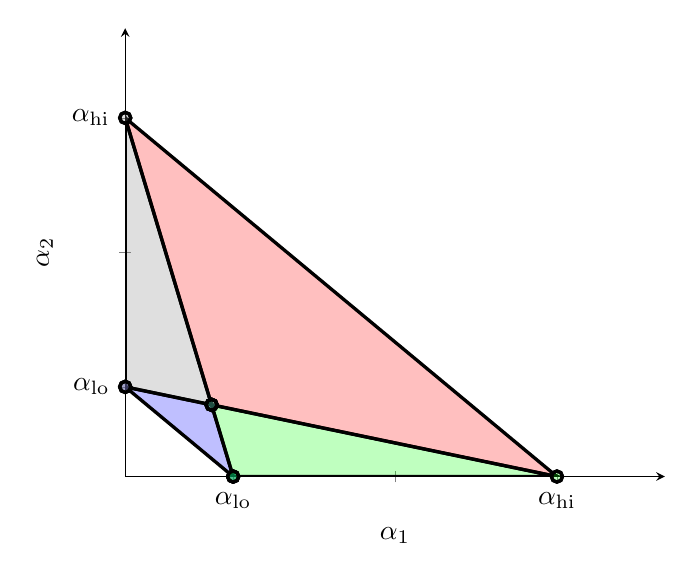
\begin{tikzpicture}
\begin{axis}[
    xmin=0, xmax=1,
    axis x line=bottom,% only show the bottom x axis
    axis y line=left,
    xlabel={$\alpha_1$},
    ylabel={$\alpha_2$},
    xtick={0.2,0.5,0.8},
    xticklabels={$\alo$,,$\ahi$},  
    ytick={0.2,0.5,0.8},
    yticklabels={$\alo$,,$\ahi$},  
    ymin=0,ymax=1,
    scatter/classes={%
        a={mark=o,draw=black}}
    ]
    \addplot [mark=*,very thick,fill=blue, fill opacity=0.25] coordinates {
        (0.2, 0)
        (0, 0.2)
        (0.16, 0.16)
        (0.2, 0)
    };
    \addplot [mark=*,very thick,fill=green, fill opacity=0.25] coordinates {
        (0.2, 0)
        (0.8, 0)
        (0.16, 0.16)
        (0.2, 0)
    };
    \addplot [mark=*,very thick,fill=gray, fill opacity=0.25] coordinates {
        (0, 0.2)
        (0, 0.8)
        (0.16, 0.16)
        (0, 0.2)
    };
    \addplot [mark=o,very thick,fill=red, fill opacity=0.25] coordinates {
        (0.16, 0.16)
        (0.8, 0)
        (0, 0.8)
        (0.16, 0.16)
    };
\end{axis}
\end{tikzpicture}
\caption{Finding the merges in the different regions can be more challenging when interpolating with two weight parameters $\alpha_1$ and $\alpha_2$.}
\label{fig:convexhulls2}
\end{figure}

In addition, we can apply the introduced algorithms to more datasets and data domains, such as the sets contained in the UCI Machine Learning Repository \cite{Dua:2019}. For instance, we could compare different datasets within one specific data domain. Say we evaluate a variety of different image datasets and compare the optimal values of $\alpha$. An interesting observation would be, if we could reuse the optimal parameter from different datasets within the same or even across other domains. In our experiments, we often found similar optimal values in the range $[0.7,0.9]$ while other ranges mostly did not lead to good results (e.g.\ $[0.0, 0.5]$). We could use this knowledge for further experiments by e.g. evaluating only smaller regions or by putting more emphasis on given parameters in general. We can then also evaluate other domains, such as (partially) labeled voice datasets (e.g. the Free Music Archive dataset \cite{fma} or LibriSpeech \cite{librispeech}) and compare the results across different data domains.\\

Also, we can imagine applying this framework to (a) other clustering algorithms than agglomerative hierarchical clustering and (b) other tasks than clustering.

%% --------------------
%% |   Bibliography   |
%% --------------------

%% Add entry to the table of contents for the bibliography
\printbibliography[heading=bibintoc]

%% ----------------
%% |   Appendix   |
%% ----------------
\appendix
\chapter{The Hungarian Method}
\label{sec:hungarian}

Our goal is to find the best possible matching between two clusterings $C_1^i, ..., C_k^i$ and $C_1^j, ..., C_k^j$. In order to do so, we calculate the cost of matching each possible pair of clusters within the two clusterings. 
% Table \ref{app:hung:distances} shows how such a cost matrix can look like.

% \begin{table}[h]
%     \centering
%     \begin{tabular}{|l | l l l l l|}
%     \hline
%     j\textbackslash i & 1 & 2 & 3 & 4 & 5\\ \hline
%     1 & 20 & 15 & 30 & 50 & 40\\
%     2 & 80 & 10 & 15 & 20 & 30\\
%     3 & 20 & 30 & 50 & 80 & 60\\
%     4 & 30 & 50 & 40 & 20 & 10\\
%     5 & 20 & 30 & 40 & 50 & 25\\ \hline
%     \end{tabular}
%     \caption{In order to determine the optimal matching between two clusterings, we note the pairwise matching costs.}
%     \label{app:hung:distances}
% \end{table}

To find the optimal matching in a brute force way, we have to look at each possible matching. Say we want to match each $i$ to one $j$. For $i = 1$ we can pick from 5 different values of $j$, for $i = 2$ there are 4 potential values of $j$. This will overall result in $k! = 5! = 120$ different combinations, thus the complexity of the brute force approach is $O(k!)$. A more efficient algorithm (especially for higher values of $k$) was introduced by Kuhn and Munkres \cite{kuhn1955hungarian}\cite{munkres1957algorithms}. It consists of three major steps. In the first one, we subtract the row minima from each row. This step is performed in table \ref{app:hung:step1}.

\begin{table}[h]
    \centering
    \begin{tabular}{|l | l l l l l| l |}
    \hline
    j\textbackslash i & 1 & 2 & 3 & 4 & 5 & \\ \hline
    1 & 5 & 0 & 15 & 35 & 25 & (-15)\\
    2 & 70 & 0 & 5 & 10 & 20 & (-10)\\
    3 & 0 & 10 & 30 & 60 & 40 & (-20)\\
    4 & 20 & 40 & 30 & 10 & 0 & (-10)\\
    5 & 0 & 10 & 20 & 30 & 5 & (-20)\\ \hline
    \end{tabular}
    \caption{Hungarian method step 1: Subtract the row minima from each row.}
    \label{app:hung:step1}
\end{table}

After subtracting the row minima, we now also subtract the column minima from each column as shown in table \ref{app:hung:step2}.

\begin{table}[h]
    \centering
    \begin{tabular}{|l | l l l l l |}
    \hline
    j\textbackslash i & 1 & 2 & 3 & 4 & 5\\ \hline
    1 & 5 & 0 & 10 & 25 & 25\\
    2 & 70 & 0 & 0 & 0 & 20\\
    3 & 0 & 10 & 25 & 50 & 40\\
    4 & 20 & 40 & 25 & 0 & 0\\
    5 & 0 & 10 & 15 & 20 & 5\\ \hline
    & - & - & (-5) & (-10) & -\\ \hline
    \end{tabular}
    \caption{Hungarian method step 2: Subtract the column minima from each column.}
    \label{app:hung:step2}
\end{table}

Now we try to find the optimal matching. To do so, we cover all zeros with lines and count the minumum needed lines to do so. Table \ref{app:hung:step3} shows that we need four lines.

\begin{table}[h]
    \centering
    \begin{tabular}{|l | l l l l l |}
    \hline
    j\textbackslash i & 1 & 2 & 3 & 4 & 5\\ \hline
    1 & \cellcolor{orange!25}5 & \cellcolor{orange!50}0 & 10 & 25 & 25\\
    2 & \cellcolor{orange!75}70 & \cellcolor{orange!75}0 & \cellcolor{orange!75}0 & \cellcolor{orange!75}0 & \cellcolor{orange!75}20\\
    3 & \cellcolor{orange!25}0 & \cellcolor{orange!50}10 & 25 & 50 & 40\\
    4 & \cellcolor{orange!75}20 & \cellcolor{orange!75}40 & \cellcolor{orange!75}25 & \cellcolor{orange!75}0 & \cellcolor{orange!75}0\\
    5 & \cellcolor{orange!25}0 & \cellcolor{orange!50}10 & 15 & 20 & 5\\ \hline
    \end{tabular}
    \caption{Hungarian method step 3: Cover all zeros with as few lines as possible.}
    \label{app:hung:step3}
\end{table}

After covering the zeros and counting the lines, we found the optimal matching in case the number of lines equals the number of rows (or columns) in the matrix. As we need four lines and the matrix has five rows in this example, we have to add more zeros. To do that, we subtract the minimum value of the matrix (which is 5 here) from all uncovered values that are not zero and add it to all values that are not zero and covered twice. Now we can again check the needed lines as in table \ref{app:hung:additionalstep}.

\begin{table}[h]
    \centering
    \begin{tabular}{|l | l l l l l |}
    \hline
    j\textbackslash i & 1 & 2 & 3 & 4 & 5\\ \hline
    1 & 5 & 0 & 5 & 20 & 20\\
    2 & 75 & 0 & 0 & 0 & 20\\
    3 & 0 & 10 & 20 & 45 & 35\\
    4 & 25 & 45 & 25 & 0 & 0\\
    5 & 0 & 10 & 10 & 15 & 0\\ \hline
    \end{tabular}
    \begin{tabular}{|l | l l l l l |}
        \hline
        j\textbackslash i & 1 & 2 & 3 & 4 & 5\\ \hline
        1 & \cellcolor{orange!25}5 & \cellcolor{orange!50}0 & 5 & 20 & 20\\
        2 & \cellcolor{orange!75}75 & \cellcolor{orange!75}0 & \cellcolor{orange!75}0 & \cellcolor{orange!75}0 & \cellcolor{orange!75}20\\
        3 & \cellcolor{orange!25}0 & \cellcolor{orange!50}10 & 20 & 45 & 35\\
        4 & \cellcolor{orange!75}25 & \cellcolor{orange!75}45 & \cellcolor{orange!75}25 & \cellcolor{orange!75}0 & \cellcolor{orange!75}0\\
        5 & \cellcolor{orange!100}0 & \cellcolor{orange!100}10 & \cellcolor{orange!100}10 & \cellcolor{orange!100}15 & \cellcolor{orange!100}0\\ \hline
    \end{tabular}
    \caption{Hungarian method additional step: Create more zeroes until the number of minimal needed lines to cover all zeros matches the number of rows.}
    \label{app:hung:additionalstep}
\end{table}

This will then result in the assignment seen in table \ref{app:hung:assignment}. Applying the matching to the input matrix then gives the optimal cost by summing the optimal values. For this example the optimal cost is then 95.

\begin{table}[h]
    \centering
    \begin{tabular}{|l | l l l l l |}
    \hline
    j\textbackslash i & 1 & 2 & 3 & 4 & 5\\ \hline
    1 & 5 & \cellcolor{blue!25}0 & 5 & 20 & 20\\
    2 & 75 & 0 & \cellcolor{blue!25}0 & 0 & 20\\
    3 & \cellcolor{blue!25}0 & 10 & 20 & 45 & 35\\
    4 & 25 & 45 & 25 & \cellcolor{blue!25}0 & 0\\
    5 & 0 & 10 & 10 & 15 & \cellcolor{blue!25}0\\ \hline
    \end{tabular}
    \begin{tabular}{|l | l l l l l|}
        \hline
        j\textbackslash i & 1 & 2 & 3 & 4 & 5\\ \hline
        1 & 20 & \cellcolor{blue!25}15 & 30 & 50 & 40\\
        2 & 80 & 10 & \cellcolor{blue!25}15 & 20 & 30\\
        3 & \cellcolor{blue!25}20 & 30 & 50 & 80 & 60\\
        4 & 30 & 50 & 40 & \cellcolor{blue!25}20 & 10\\
        5 & 20 & 30 & 40 & 50 & \cellcolor{blue!25}25\\ \hline
    \end{tabular}
    \caption{Result of the Hungarian method: The optimal matching between two clusterings.}
    \label{app:hung:assignment}
\end{table}	% Appendix Title

\chapter{Proposed NELL Subcategories}
\label{sec:nellsubcategories}

\begin{table}[H]
  \makebox[\textwidth][c]{
  \small
  \begin{tabular}{cccc}
    \hline\hline
    \textbf{Luxury Room} & \textbf{Bathroom} & \textbf{Guest Room} & \textbf{Suite} \\ \hline
    spacious living room & large ensuite bathroom & elegant rooms & luxurious suites\\
    comfortable living room & spacious marble bathroom & three guest rooms & one bedroom suites\\
    guest room & one bathroom & large guest rooms & spacious suites\\
    lounge room & full bathroom & deluxe guest rooms & deluxe suites\\
    living room & upstairs bathroom & guests rooms & guest suites\\
    superior room & large bathroom & spacious air conditioned rooms & bedroom suites\\
    sleeping room & ensuite bathroom & furnished guest rooms & whirlpool suites\\
    main bedroom & elegant bathroom & comfortable guest rooms & three suites\\
    \hline
  \end{tabular}
  }
  \caption{Proposed Subcategories for ``Office Building Room''.}
  \label{tbl:rooms}
\end{table}

\begin{table}[H]
  \makebox[\textwidth][c]{
  \small
  \begin{tabular}{ccccc}
    \hline\hline
    \textbf{Shoes} & \textbf{Uniform/Costume} & \textbf{Pants} & \textbf{Casual} & \textbf{Specialized} \\ \hline
    shoes & costume & kneepants & stocking cap & long stockings\\
    high heel shoes & work uniforms & baggy pants & workout clothes & wide brimmed hat\\
    sensible shoes & outfits & loose fitting pants & casual clothes & casual wear\\
    old shoes & period costume & slacks & baseball caps & black stockings\\
    pointe shoes & folk costumes & black shorts & skull caps & wear socks\\
    dark shoes & halter top & special clothing & ball caps & high heels\\
    spira shoes & period costumes & white shorts & evening clothes & surf wear\\
    mens shoes & costumes & underpants & ball cap & wear gloves\\
    \hline
  \end{tabular}
  }
  \caption{Proposed Subcategories for ``Clothing''.}
  \label{tbl:clothing}
\end{table}

\begin{table}[H]
  \makebox[\textwidth][c]{
  \small
  \begin{tabular}{cccc}
    \hline\hline
    \textbf{Stove/Oven} & \textbf{Machines} & \textbf{Bowls} & \textbf{Baking Sheets} \\ \hline
    full size stove & cookie cutters & large mixing bowl & oiled baking sheet\\
    full size cooker & automatic washing machine & large serving bowl & rimmed baking sheet\\
    red hot stove & washing machine & small bowl & large baking sheet\\
    plastic jug & bread machine & single bowl & small baking sheet\\
    toaster & cookie cutter & separate bowl & prepared baking sheet\\
    greased baking dish & coffee machine & shallow bowl & ungreased baking sheet\\
    wood burning pizza oven & cooking spray & separate mixing bowl & hot plate\\
    ceramic top stove & coffee grinder & large bowl & greased baking sheet\\
    \hline
  \end{tabular}
  }
  \caption{Proposed Subcategories for ``Kitchen Item''.}
  \label{tbl:kitchenitems}
\end{table} % Appendix Title

\chapter{Additional NELL Results}
\label{app:nell}

Here we show the results of all the 32 different used entities. We used a maximum of 1,000 points for each entity, however for some of them less samples were given. We show both interpolating between average and complete and between single and complete linkage in the following figures.

\begin{figure}[h]
\centering
\begin{minipage}{.24\textwidth}
  \centering
  \subcaptionbox{Animal}
  {\includegraphics[width=\linewidth]{plots/nell-ac/animal}}
\end{minipage}
\begin{minipage}{.24\textwidth}
  \centering
  \subcaptionbox{Arthropod}
  {\includegraphics[width=\linewidth]{plots/nell-ac/arthropod}}
\end{minipage}
\begin{minipage}{.24\textwidth}
  \centering
  \subcaptionbox{Attraction}
  {\includegraphics[width=\linewidth]{plots/nell-ac/attraction}}
\end{minipage}
\begin{minipage}{.24\textwidth}
  \centering
  \subcaptionbox{Beverage}
  {\includegraphics[width=\linewidth]{plots/nell-ac/beverage}}
\end{minipage}
\begin{minipage}{.24\textwidth}
  \centering
  \subcaptionbox{Bodypart}
  {\includegraphics[width=\linewidth]{plots/nell-ac/bodypart}}
\end{minipage}
\begin{minipage}{.24\textwidth}
  \centering
  \subcaptionbox{Building}
  {\includegraphics[width=\linewidth]{plots/nell-ac/building}}
\end{minipage}
\begin{minipage}{.24\textwidth}
  \centering
  \subcaptionbox{Company}
  {\includegraphics[width=\linewidth]{plots/nell-ac/company}}
\end{minipage}
\begin{minipage}{.24\textwidth}
  \centering
  \subcaptionbox{Creative Work}
  {\includegraphics[width=\linewidth]{plots/nell-ac/creativework}}
\end{minipage}
\begin{minipage}{.24\textwidth}
  \centering
  \subcaptionbox{Date}
  {\includegraphics[width=\linewidth]{plots/nell-ac/date}}
\end{minipage}
\begin{minipage}{.24\textwidth}
  \centering
  \subcaptionbox{Event}
  {\includegraphics[width=\linewidth]{plots/nell-ac/event}}
\end{minipage}
\begin{minipage}{.24\textwidth}
  \centering
  \subcaptionbox{Food}
  {\includegraphics[width=\linewidth]{plots/nell-ac/food}}
\end{minipage}
\begin{minipage}{.24\textwidth}
  \centering
  \subcaptionbox{Fruit}
  {\includegraphics[width=\linewidth]{plots/nell-ac/fruit}}
\end{minipage}
\begin{minipage}{.24\textwidth}
  \centering
  \subcaptionbox{Game}
  {\includegraphics[width=\linewidth]{plots/nell-ac/game}}
\end{minipage}
\begin{minipage}{.24\textwidth}
  \centering
  \subcaptionbox{Household Item}
  {\includegraphics[width=\linewidth]{plots/nell-ac/householditem}}
\end{minipage}
\begin{minipage}{.24\textwidth}
  \centering
  \subcaptionbox{Invertebrate}
  {\includegraphics[width=\linewidth]{plots/nell-ac/invertebrate}}
\end{minipage}
\begin{minipage}{.24\textwidth}
  \centering
  \subcaptionbox{Location}
  {\includegraphics[width=\linewidth]{plots/nell-ac/location}}
\end{minipage}
\end{figure}
\begin{figure}[h]\ContinuedFloat
\centering
\begin{minipage}{.24\textwidth}
  \centering
  \subcaptionbox{Mediacompany}
  {\includegraphics[width=\linewidth]{plots/nell-ac/mediacompany}}
\end{minipage}
\begin{minipage}{.24\textwidth}
  \centering
  \subcaptionbox{Organization}
  {\includegraphics[width=\linewidth]{plots/nell-ac/organization}}
\end{minipage}
\begin{minipage}{.24\textwidth}
  \centering
  \subcaptionbox{Person}
  {\includegraphics[width=\linewidth]{plots/nell-ac/person}}
\end{minipage}
\begin{minipage}{.24\textwidth}
  \centering
  \subcaptionbox{Person by Location}
  {\includegraphics[width=\linewidth]{plots/nell-ac/personbylocation}}
\end{minipage}
\begin{minipage}{.24\textwidth}
  \centering
  \subcaptionbox{Person NA}
  {\includegraphics[width=\linewidth]{plots/nell-ac/personnorthamerica}}
\end{minipage}
\begin{minipage}{.24\textwidth}
  \centering
  \subcaptionbox{Physiological Condition}
  {\includegraphics[width=\linewidth]{plots/nell-ac/physiologicalcondition}}
\end{minipage}
\begin{minipage}{.24\textwidth}
  \centering
  \subcaptionbox{Politics Group}
  {\includegraphics[width=\linewidth]{plots/nell-ac/politicsgroup}}
\end{minipage}
\begin{minipage}{.24\textwidth}
  \centering
  \subcaptionbox{Product}
  {\includegraphics[width=\linewidth]{plots/nell-ac/Product}}
\end{minipage}
\begin{minipage}{.24\textwidth}
  \centering
  \subcaptionbox{Publication}
  {\includegraphics[width=\linewidth]{plots/nell-ac/publication}}
\end{minipage}
\begin{minipage}{.24\textwidth}
  \centering
  \subcaptionbox{School}
  {\includegraphics[width=\linewidth]{plots/nell-ac/school}}
\end{minipage}
\begin{minipage}{.24\textwidth}
  \centering
  \subcaptionbox{Software}
  {\includegraphics[width=\linewidth]{plots/nell-ac/software}}
\end{minipage}
\begin{minipage}{.24\textwidth}
  \centering
  \subcaptionbox{Sports Event}
  {\includegraphics[width=\linewidth]{plots/nell-ac/sportsevent}}
\end{minipage}
\begin{minipage}{.24\textwidth}
  \centering
  \subcaptionbox{Traditional Game}
  {\includegraphics[width=\linewidth]{plots/nell-ac/traditionalgame}}
\end{minipage}
\begin{minipage}{.24\textwidth}
  \centering
  \subcaptionbox{Vertebrate}
  {\includegraphics[width=\linewidth]{plots/nell-ac/vertebrate}}
\end{minipage}
\begin{minipage}{.24\textwidth}
  \centering
  \subcaptionbox{Visualizable Attribute}
  {\includegraphics[width=\linewidth]{plots/nell-ac/visualizableattribute}}
\end{minipage}
\begin{minipage}{.24\textwidth}
  \centering
  \subcaptionbox{Website}
  {\includegraphics[width=\linewidth]{plots/nell-ac/website}}
\end{minipage}
\caption{Interpolating between average and complete linkage for the NELL data.}
\end{figure}

\begin{figure}[h]
\centering
\begin{minipage}{.24\textwidth}
  \centering
  \subcaptionbox{Animal}
  {\includegraphics[width=\linewidth]{plots/nell-sc/animal}}
\end{minipage}
\begin{minipage}{.24\textwidth}
  \centering
  \subcaptionbox{Arthropod}
  {\includegraphics[width=\linewidth]{plots/nell-sc/arthropod}}
\end{minipage}
\begin{minipage}{.24\textwidth}
  \centering
  \subcaptionbox{Attraction}
  {\includegraphics[width=\linewidth]{plots/nell-sc/attraction}}
\end{minipage}
\begin{minipage}{.24\textwidth}
  \centering
  \subcaptionbox{Beverage}
  {\includegraphics[width=\linewidth]{plots/nell-sc/beverage}}
\end{minipage}
\begin{minipage}{.24\textwidth}
  \centering
  \subcaptionbox{Bodypart}
  {\includegraphics[width=\linewidth]{plots/nell-sc/bodypart}}
\end{minipage}
\begin{minipage}{.24\textwidth}
  \centering
  \subcaptionbox{Building}
  {\includegraphics[width=\linewidth]{plots/nell-sc/building}}
\end{minipage}
\begin{minipage}{.24\textwidth}
  \centering
  \subcaptionbox{Company}
  {\includegraphics[width=\linewidth]{plots/nell-sc/company}}
\end{minipage}
\begin{minipage}{.24\textwidth}
  \centering
  \subcaptionbox{Creative Work}
  {\includegraphics[width=\linewidth]{plots/nell-sc/creativework}}
\end{minipage}
\begin{minipage}{.24\textwidth}
  \centering
  \subcaptionbox{Date}
  {\includegraphics[width=\linewidth]{plots/nell-sc/date}}
\end{minipage}
\begin{minipage}{.24\textwidth}
  \centering
  \subcaptionbox{Event}
  {\includegraphics[width=\linewidth]{plots/nell-sc/event}}
\end{minipage}
\begin{minipage}{.24\textwidth}
  \centering
  \subcaptionbox{Food}
  {\includegraphics[width=\linewidth]{plots/nell-sc/food}}
\end{minipage}
\begin{minipage}{.24\textwidth}
  \centering
  \subcaptionbox{Fruit}
  {\includegraphics[width=\linewidth]{plots/nell-sc/fruit}}
\end{minipage}
\begin{minipage}{.24\textwidth}
  \centering
  \subcaptionbox{Game}
  {\includegraphics[width=\linewidth]{plots/nell-sc/game}}
\end{minipage}
\begin{minipage}{.24\textwidth}
  \centering
  \subcaptionbox{Household Item}
  {\includegraphics[width=\linewidth]{plots/nell-sc/householditem}}
\end{minipage}
\begin{minipage}{.24\textwidth}
  \centering
  \subcaptionbox{Invertebrate}
  {\includegraphics[width=\linewidth]{plots/nell-sc/invertebrate}}
\end{minipage}
\begin{minipage}{.24\textwidth}
  \centering
  \subcaptionbox{Location}
  {\includegraphics[width=\linewidth]{plots/nell-sc/location}}
\end{minipage}
\begin{minipage}{.24\textwidth}
  \centering
  \subcaptionbox{Mediacompany}
  {\includegraphics[width=\linewidth]{plots/nell-sc/mediacompany}}
\end{minipage}
\begin{minipage}{.24\textwidth}
  \centering
  \subcaptionbox{Organization}
  {\includegraphics[width=\linewidth]{plots/nell-sc/organization}}
\end{minipage}
\begin{minipage}{.24\textwidth}
  \centering
  \subcaptionbox{Person}
  {\includegraphics[width=\linewidth]{plots/nell-sc/person}}
\end{minipage}
\begin{minipage}{.24\textwidth}
  \centering
  \subcaptionbox{Person by Location}
  {\includegraphics[width=\linewidth]{plots/nell-sc/personbylocation}}
\end{minipage}
\end{figure}
\begin{figure}[h]\ContinuedFloat
\centering
\begin{minipage}{.24\textwidth}
  \centering
  \subcaptionbox{Person NA}
  {\includegraphics[width=\linewidth]{plots/nell-sc/personnorthamerica}}
\end{minipage}
\begin{minipage}{.24\textwidth}
  \centering
  \subcaptionbox{Physiological Condition}
  {\includegraphics[width=\linewidth]{plots/nell-sc/physiologicalcondition}}
\end{minipage}
\begin{minipage}{.24\textwidth}
  \centering
  \subcaptionbox{Politics Group}
  {\includegraphics[width=\linewidth]{plots/nell-sc/politicsgroup}}
\end{minipage}
\begin{minipage}{.24\textwidth}
  \centering
  \subcaptionbox{Product}
  {\includegraphics[width=\linewidth]{plots/nell-sc/Product}}
\end{minipage}
\begin{minipage}{.24\textwidth}
  \centering
  \subcaptionbox{Publication}
  {\includegraphics[width=\linewidth]{plots/nell-sc/publication}}
\end{minipage}
\begin{minipage}{.24\textwidth}
  \centering
  \subcaptionbox{School}
  {\includegraphics[width=\linewidth]{plots/nell-sc/school}}
\end{minipage}
\begin{minipage}{.24\textwidth}
  \centering
  \subcaptionbox{Software}
  {\includegraphics[width=\linewidth]{plots/nell-sc/software}}
\end{minipage}
\begin{minipage}{.24\textwidth}
  \centering
  \subcaptionbox{Sports Event}
  {\includegraphics[width=\linewidth]{plots/nell-sc/sportsevent}}
\end{minipage}
\begin{minipage}{.24\textwidth}
  \centering
  \subcaptionbox{Traditional Game}
  {\includegraphics[width=\linewidth]{plots/nell-sc/traditionalgame}}
\end{minipage}
\begin{minipage}{.24\textwidth}
  \centering
  \subcaptionbox{Vertebrate}
  {\includegraphics[width=\linewidth]{plots/nell-sc/vertebrate}}
\end{minipage}
\begin{minipage}{.24\textwidth}
  \centering
  \subcaptionbox{Visualizable Attribute}
  {\includegraphics[width=\linewidth]{plots/nell-sc/visualizableattribute}}
\end{minipage}
\begin{minipage}{.24\textwidth}
  \centering
  \subcaptionbox{Website}
  {\includegraphics[width=\linewidth]{plots/nell-sc/website}}
\end{minipage}
\caption{Interpolating between single and complete linkage for the NELL data.}
\end{figure} % Appendix Title

\chapter{Omniglot Intra-Alphabet Results}
\label{app:omniglot}

\begin{figure}[H]
\centering
\begin{minipage}{.24\textwidth}
  \centering
  \subcaptionbox{Magi}
  {\includegraphics[width=\linewidth]{plots/omniglot-intra-ac/Alphabet_of_the_Magi}}
\end{minipage}
\begin{minipage}{.24\textwidth}
  \centering
  \subcaptionbox{Anglo-Saxon}
  {\includegraphics[width=\linewidth]{plots/omniglot-intra-ac/Anglo-Saxon_Futhorc}}
\end{minipage}
\begin{minipage}{.24\textwidth}
  \centering
  \subcaptionbox{Arcadian}
  {\includegraphics[width=\linewidth]{plots/omniglot-intra-ac/Arcadian}}
\end{minipage}
\begin{minipage}{.24\textwidth}
  \centering
  \subcaptionbox{Armenian}
  {\includegraphics[width=\linewidth]{plots/omniglot-intra-ac/Armenian}}
\end{minipage}
\begin{minipage}{.24\textwidth}
  \centering
  \subcaptionbox{Asomtavruli}
  {\includegraphics[width=\linewidth]{plots/omniglot-intra-ac/Asomtavruli_(Georgian)}}
\end{minipage}
\begin{minipage}{.24\textwidth}
  \centering
  \subcaptionbox{Balinese}
  {\includegraphics[width=\linewidth]{plots/omniglot-intra-ac/Balinese}}
\end{minipage}
\begin{minipage}{.24\textwidth}
  \centering
  \subcaptionbox{Bengali}
  {\includegraphics[width=\linewidth]{plots/omniglot-intra-ac/Bengali}}
\end{minipage}
\begin{minipage}{.24\textwidth}
  \centering
  \subcaptionbox{Blackfoot}
  {\includegraphics[width=\linewidth]{plots/omniglot-intra-ac/Blackfoot_(Canadian_Aboriginal_Syllabics)}}
\end{minipage}
\begin{minipage}{.24\textwidth}
  \centering
  \subcaptionbox{Braille}
  {\includegraphics[width=\linewidth]{plots/omniglot-intra-ac/Braille}}
\end{minipage}
\begin{minipage}{.24\textwidth}
  \centering
  \subcaptionbox{Burmese}
  {\includegraphics[width=\linewidth]{plots/omniglot-intra-ac/Burmese_(Myanmar)}}
\end{minipage}
\begin{minipage}{.24\textwidth}
  \centering
  \subcaptionbox{Cyrillic}
  {\includegraphics[width=\linewidth]{plots/omniglot-intra-ac/Cyrillic}}
\end{minipage}
\begin{minipage}{.24\textwidth}
  \centering
  \subcaptionbox{Early\_Aramaic}
  {\includegraphics[width=\linewidth]{plots/omniglot-intra-ac/Early_Aramaic}}
\end{minipage}
\begin{minipage}{.24\textwidth}
  \centering
  \subcaptionbox{Futurama}
  {\includegraphics[width=\linewidth]{plots/omniglot-intra-ac/Futurama}}
\end{minipage}
\begin{minipage}{.24\textwidth}
  \centering
  \subcaptionbox{Grantha}
  {\includegraphics[width=\linewidth]{plots/omniglot-intra-ac/Grantha}}
\end{minipage}
\begin{minipage}{.24\textwidth}
  \centering
  \subcaptionbox{Greek}
  {\includegraphics[width=\linewidth]{plots/omniglot-intra-ac/Greek}}
\end{minipage}
\begin{minipage}{.24\textwidth}
  \centering
  \subcaptionbox{Gujarati}
  {\includegraphics[width=\linewidth]{plots/omniglot-intra-ac/Gujarati}}
\end{minipage}
\begin{minipage}{.24\textwidth}
  \centering
  \subcaptionbox{Hebrew}
  {\includegraphics[width=\linewidth]{plots/omniglot-intra-ac/Hebrew}}
\end{minipage}
\begin{minipage}{.24\textwidth}
  \centering
  \subcaptionbox{Inuktitut}
  {\includegraphics[width=\linewidth]{plots/omniglot-intra-ac/Inuktitut_(Canadian_Aboriginal_Syllabics)}}
\end{minipage}
\begin{minipage}{.24\textwidth}
  \centering
  \subcaptionbox{Hiragana}
  {\includegraphics[width=\linewidth]{plots/omniglot-intra-ac/Japanese_(hiragana)}}
\end{minipage}
\begin{minipage}{.24\textwidth}
  \centering
  \subcaptionbox{Katakana}
  {\includegraphics[width=\linewidth]{plots/omniglot-intra-ac/Japanese_(katakana)}}
\end{minipage}
\end{figure}
\begin{figure}[H]\ContinuedFloat
\centering
\begin{minipage}{.24\textwidth}
  \centering
  \subcaptionbox{Korean}
  {\includegraphics[width=\linewidth]{plots/omniglot-intra-ac/Korean}}
\end{minipage}
\begin{minipage}{.24\textwidth}
  \centering
  \subcaptionbox{Latin}
  {\includegraphics[width=\linewidth]{plots/omniglot-intra-ac/Latin}}
\end{minipage}
\begin{minipage}{.24\textwidth}
  \centering
  \subcaptionbox{Malay}
  {\includegraphics[width=\linewidth]{plots/omniglot-intra-ac/Malay_(Jawi_-_Arabic)}}
\end{minipage}
\begin{minipage}{.24\textwidth}
  \centering
  \subcaptionbox{Mkhedruli}
  {\includegraphics[width=\linewidth]{plots/omniglot-intra-ac/Mkhedruli_(Georgian)}}
\end{minipage}
\begin{minipage}{.24\textwidth}
  \centering
  \subcaptionbox{N\_Ko}
  {\includegraphics[width=\linewidth]{plots/omniglot-intra-ac/N_Ko}}
\end{minipage}
\begin{minipage}{.24\textwidth}
  \centering
  \subcaptionbox{Ojibwe}
  {\includegraphics[width=\linewidth]{plots/omniglot-intra-ac/Ojibwe_(Canadian_Aboriginal_Syllabics)}}
\end{minipage}
\begin{minipage}{.24\textwidth}
  \centering
  \subcaptionbox{Sanskrit}
  {\includegraphics[width=\linewidth]{plots/omniglot-intra-ac/Sanskrit}}
\end{minipage}
\begin{minipage}{.24\textwidth}
  \centering
  \subcaptionbox{Syriac}
  {\includegraphics[width=\linewidth]{plots/omniglot-intra-ac/Syriac_(Estrangelo)}}
\end{minipage}
\begin{minipage}{.24\textwidth}
  \centering
  \subcaptionbox{Tagalog}
  {\includegraphics[width=\linewidth]{plots/omniglot-intra-ac/Tagalog}}
\end{minipage}
\begin{minipage}{.24\textwidth}
  \centering
  \subcaptionbox{Tifinagh}
  {\includegraphics[width=\linewidth]{plots/omniglot-intra-ac/Tifinagh}}
\end{minipage}
\caption{%
  %
  Interpolating between average and complete linkage for the omniglot data.}
  %
\label{}
\end{figure}

\begin{figure}[H]
\centering
\begin{minipage}{.24\textwidth}
  \centering
  \subcaptionbox{Magi}
  {\includegraphics[width=\linewidth]{plots/omniglot-intra-sc/Alphabet_of_the_Magi}}
\end{minipage}
\begin{minipage}{.24\textwidth}
  \centering
  \subcaptionbox{Anglo-Saxon}
  {\includegraphics[width=\linewidth]{plots/omniglot-intra-sc/Anglo-Saxon_Futhorc}}
\end{minipage}
\begin{minipage}{.24\textwidth}
  \centering
  \subcaptionbox{Arcadian}
  {\includegraphics[width=\linewidth]{plots/omniglot-intra-sc/Arcadian}}
\end{minipage}
\begin{minipage}{.24\textwidth}
  \centering
  \subcaptionbox{Armenian}
  {\includegraphics[width=\linewidth]{plots/omniglot-intra-sc/Armenian}}
\end{minipage}
\begin{minipage}{.24\textwidth}
  \centering
  \subcaptionbox{Asomtavruli}
  {\includegraphics[width=\linewidth]{plots/omniglot-intra-sc/Asomtavruli_(Georgian)}}
\end{minipage}
\begin{minipage}{.24\textwidth}
  \centering
  \subcaptionbox{Balinese}
  {\includegraphics[width=\linewidth]{plots/omniglot-intra-sc/Balinese}}
\end{minipage}
\begin{minipage}{.24\textwidth}
  \centering
  \subcaptionbox{Bengali}
  {\includegraphics[width=\linewidth]{plots/omniglot-intra-sc/Bengali}}
\end{minipage}
\begin{minipage}{.24\textwidth}
  \centering
  \subcaptionbox{Blackfoot}
  {\includegraphics[width=\linewidth]{plots/omniglot-intra-sc/Blackfoot_(Canadian_Aboriginal_Syllabics)}}
\end{minipage}
\begin{minipage}{.24\textwidth}
  \centering
  \subcaptionbox{Braille}
  {\includegraphics[width=\linewidth]{plots/omniglot-intra-sc/Braille}}
\end{minipage}
\begin{minipage}{.24\textwidth}
  \centering
  \subcaptionbox{Burmese}
  {\includegraphics[width=\linewidth]{plots/omniglot-intra-sc/Burmese_(Myanmar)}}
\end{minipage}
\begin{minipage}{.24\textwidth}
  \centering
  \subcaptionbox{Cyrillic}
  {\includegraphics[width=\linewidth]{plots/omniglot-intra-sc/Cyrillic}}
\end{minipage}
\begin{minipage}{.24\textwidth}
  \centering
  \subcaptionbox{Early\_Aramaic}
  {\includegraphics[width=\linewidth]{plots/omniglot-intra-sc/Early_Aramaic}}
\end{minipage}
\begin{minipage}{.24\textwidth}
  \centering
  \subcaptionbox{Futurama}
  {\includegraphics[width=\linewidth]{plots/omniglot-intra-sc/Futurama}}
\end{minipage}
\begin{minipage}{.24\textwidth}
  \centering
  \subcaptionbox{Grantha}
  {\includegraphics[width=\linewidth]{plots/omniglot-intra-sc/Grantha}}
\end{minipage}
\begin{minipage}{.24\textwidth}
  \centering
  \subcaptionbox{Greek}
  {\includegraphics[width=\linewidth]{plots/omniglot-intra-sc/Greek}}
\end{minipage}
\begin{minipage}{.24\textwidth}
  \centering
  \subcaptionbox{Gujarati}
  {\includegraphics[width=\linewidth]{plots/omniglot-intra-sc/Gujarati}}
\end{minipage}
\begin{minipage}{.24\textwidth}
  \centering
  \subcaptionbox{Hebrew}
  {\includegraphics[width=\linewidth]{plots/omniglot-intra-sc/Hebrew}}
\end{minipage}
\begin{minipage}{.24\textwidth}
  \centering
  \subcaptionbox{Inuktitut}
  {\includegraphics[width=\linewidth]{plots/omniglot-intra-sc/Inuktitut_(Canadian_Aboriginal_Syllabics)}}
\end{minipage}
\begin{minipage}{.24\textwidth}
  \centering
  \subcaptionbox{Hiragana}
  {\includegraphics[width=\linewidth]{plots/omniglot-intra-sc/Japanese_(hiragana)}}
\end{minipage}
\begin{minipage}{.24\textwidth}
  \centering
  \subcaptionbox{Katakana}
  {\includegraphics[width=\linewidth]{plots/omniglot-intra-sc/Japanese_(katakana)}}
\end{minipage}
\end{figure}
\begin{figure}[H]\ContinuedFloat
\centering
\begin{minipage}{.24\textwidth}
  \centering
  \subcaptionbox{Korean}
  {\includegraphics[width=\linewidth]{plots/omniglot-intra-sc/Korean}}
\end{minipage}
\begin{minipage}{.24\textwidth}
  \centering
  \subcaptionbox{Latin}
  {\includegraphics[width=\linewidth]{plots/omniglot-intra-sc/Latin}}
\end{minipage}
\begin{minipage}{.24\textwidth}
  \centering
  \subcaptionbox{Malay}
  {\includegraphics[width=\linewidth]{plots/omniglot-intra-sc/Malay_(Jawi_-_Arabic)}}
\end{minipage}
\begin{minipage}{.24\textwidth}
  \centering
  \subcaptionbox{Mkhedruli}
  {\includegraphics[width=\linewidth]{plots/omniglot-intra-sc/Mkhedruli_(Georgian)}}
\end{minipage}
\begin{minipage}{.24\textwidth}
  \centering
  \subcaptionbox{N\_Ko}
  {\includegraphics[width=\linewidth]{plots/omniglot-intra-sc/N_Ko}}
\end{minipage}
\begin{minipage}{.24\textwidth}
  \centering
  \subcaptionbox{Ojibwe}
  {\includegraphics[width=\linewidth]{plots/omniglot-intra-sc/Ojibwe_(Canadian_Aboriginal_Syllabics)}}
\end{minipage}
\begin{minipage}{.24\textwidth}
  \centering
  \subcaptionbox{Sanskrit}
  {\includegraphics[width=\linewidth]{plots/omniglot-intra-sc/Sanskrit}}
\end{minipage}
\begin{minipage}{.24\textwidth}
  \centering
  \subcaptionbox{Syriac}
  {\includegraphics[width=\linewidth]{plots/omniglot-intra-sc/Syriac_(Estrangelo)}}
\end{minipage}
\begin{minipage}{.24\textwidth}
  \centering
  \subcaptionbox{Tagalog}
  {\includegraphics[width=\linewidth]{plots/omniglot-intra-sc/Tagalog}}
\end{minipage}
\begin{minipage}{.24\textwidth}
  \centering
  \subcaptionbox{Tifinagh}
  {\includegraphics[width=\linewidth]{plots/omniglot-intra-sc/Tifinagh}}
\end{minipage}
\caption{%
  %
  Interpolating between single and complete linkage for the omniglot data.}
  %
\label{}
\end{figure}

\begin{figure}[H]
\centering
\begin{minipage}{.24\textwidth}
  \centering
  \subcaptionbox{Magi}
  {\includegraphics[width=\linewidth]{plots/omniglot-intra-ac-cnn/Alphabet_of_the_Magi}}
\end{minipage}
\begin{minipage}{.24\textwidth}
  \centering
  \subcaptionbox{Anglo-Saxon}
  {\includegraphics[width=\linewidth]{plots/omniglot-intra-ac-cnn/Anglo-Saxon_Futhorc}}
\end{minipage}
\begin{minipage}{.24\textwidth}
  \centering
  \subcaptionbox{Arcadian}
  {\includegraphics[width=\linewidth]{plots/omniglot-intra-ac-cnn/Arcadian}}
\end{minipage}
\begin{minipage}{.24\textwidth}
  \centering
  \subcaptionbox{Armenian}
  {\includegraphics[width=\linewidth]{plots/omniglot-intra-ac-cnn/Armenian}}
\end{minipage}
\begin{minipage}{.24\textwidth}
  \centering
  \subcaptionbox{Asomtavruli}
  {\includegraphics[width=\linewidth]{plots/omniglot-intra-ac-cnn/Asomtavruli_(Georgian)}}
\end{minipage}
\begin{minipage}{.24\textwidth}
  \centering
  \subcaptionbox{Balinese}
  {\includegraphics[width=\linewidth]{plots/omniglot-intra-ac-cnn/Balinese}}
\end{minipage}
\begin{minipage}{.24\textwidth}
  \centering
  \subcaptionbox{Bengali}
  {\includegraphics[width=\linewidth]{plots/omniglot-intra-ac-cnn/Bengali}}
\end{minipage}
\begin{minipage}{.24\textwidth}
  \centering
  \subcaptionbox{Blackfoot}
  {\includegraphics[width=\linewidth]{plots/omniglot-intra-ac-cnn/Blackfoot_(Canadian_Aboriginal_Syllabics)}}
\end{minipage}
\begin{minipage}{.24\textwidth}
  \centering
  \subcaptionbox{Braille}
  {\includegraphics[width=\linewidth]{plots/omniglot-intra-ac-cnn/Braille}}
\end{minipage}
\begin{minipage}{.24\textwidth}
  \centering
  \subcaptionbox{Burmese}
  {\includegraphics[width=\linewidth]{plots/omniglot-intra-ac-cnn/Burmese_(Myanmar)}}
\end{minipage}
\begin{minipage}{.24\textwidth}
  \centering
  \subcaptionbox{Cyrillic}
  {\includegraphics[width=\linewidth]{plots/omniglot-intra-ac-cnn/Cyrillic}}
\end{minipage}
\begin{minipage}{.24\textwidth}
  \centering
  \subcaptionbox{Early\_Aramaic}
  {\includegraphics[width=\linewidth]{plots/omniglot-intra-ac-cnn/Early_Aramaic}}
\end{minipage}
\end{figure}
\begin{figure}[H]\ContinuedFloat
\centering
\begin{minipage}{.24\textwidth}
  \centering
  \subcaptionbox{Futurama}
  {\includegraphics[width=\linewidth]{plots/omniglot-intra-ac-cnn/Futurama}}
\end{minipage}
\begin{minipage}{.24\textwidth}
  \centering
  \subcaptionbox{Grantha}
  {\includegraphics[width=\linewidth]{plots/omniglot-intra-ac-cnn/Grantha}}
\end{minipage}
\begin{minipage}{.24\textwidth}
  \centering
  \subcaptionbox{Greek}
  {\includegraphics[width=\linewidth]{plots/omniglot-intra-ac-cnn/Greek}}
\end{minipage}
\begin{minipage}{.24\textwidth}
  \centering
  \subcaptionbox{Gujarati}
  {\includegraphics[width=\linewidth]{plots/omniglot-intra-ac-cnn/Gujarati}}
\end{minipage}
\begin{minipage}{.24\textwidth}
  \centering
  \subcaptionbox{Hebrew}
  {\includegraphics[width=\linewidth]{plots/omniglot-intra-ac-cnn/Hebrew}}
\end{minipage}
\begin{minipage}{.24\textwidth}
  \centering
  \subcaptionbox{Inuktitut}
  {\includegraphics[width=\linewidth]{plots/omniglot-intra-ac-cnn/Inuktitut_(Canadian_Aboriginal_Syllabics)}}
\end{minipage}
\begin{minipage}{.24\textwidth}
  \centering
  \subcaptionbox{Hiragana}
  {\includegraphics[width=\linewidth]{plots/omniglot-intra-ac-cnn/Japanese_(hiragana)}}
\end{minipage}
\begin{minipage}{.24\textwidth}
  \centering
  \subcaptionbox{Katakana}
  {\includegraphics[width=\linewidth]{plots/omniglot-intra-ac-cnn/Japanese_(katakana)}}
\end{minipage}
\begin{minipage}{.24\textwidth}
  \centering
  \subcaptionbox{Korean}
  {\includegraphics[width=\linewidth]{plots/omniglot-intra-ac-cnn/Korean}}
\end{minipage}
\begin{minipage}{.24\textwidth}
  \centering
  \subcaptionbox{Latin}
  {\includegraphics[width=\linewidth]{plots/omniglot-intra-ac-cnn/Latin}}
\end{minipage}
\begin{minipage}{.24\textwidth}
  \centering
  \subcaptionbox{Malay}
  {\includegraphics[width=\linewidth]{plots/omniglot-intra-ac-cnn/Malay_(Jawi_-_Arabic)}}
\end{minipage}
\begin{minipage}{.24\textwidth}
  \centering
  \subcaptionbox{Mkhedruli}
  {\includegraphics[width=\linewidth]{plots/omniglot-intra-ac-cnn/Mkhedruli_(Georgian)}}
\end{minipage}
\begin{minipage}{.24\textwidth}
  \centering
  \subcaptionbox{N\_Ko}
  {\includegraphics[width=\linewidth]{plots/omniglot-intra-ac-cnn/N_Ko}}
\end{minipage}
\begin{minipage}{.24\textwidth}
  \centering
  \subcaptionbox{Ojibwe}
  {\includegraphics[width=\linewidth]{plots/omniglot-intra-ac-cnn/Ojibwe_(Canadian_Aboriginal_Syllabics)}}
\end{minipage}
\begin{minipage}{.24\textwidth}
  \centering
  \subcaptionbox{Sanskrit}
  {\includegraphics[width=\linewidth]{plots/omniglot-intra-ac-cnn/Sanskrit}}
\end{minipage}
\begin{minipage}{.24\textwidth}
  \centering
  \subcaptionbox{Syriac}
  {\includegraphics[width=\linewidth]{plots/omniglot-intra-ac-cnn/Syriac_(Estrangelo)}}
\end{minipage}
\begin{minipage}{.24\textwidth}
  \centering
  \subcaptionbox{Tagalog}
  {\includegraphics[width=\linewidth]{plots/omniglot-intra-ac-cnn/Tagalog}}
\end{minipage}
\begin{minipage}{.24\textwidth}
  \centering
  \subcaptionbox{Tifinagh}
  {\includegraphics[width=\linewidth]{plots/omniglot-intra-ac-cnn/Tifinagh}}
\end{minipage}
\caption{%
  %
  Interpolating between average and complete linkage for the omniglot data with CNN features.}
  %
\label{}
\end{figure}

\begin{figure}[H]
\centering
\begin{minipage}{.24\textwidth}
  \centering
  \subcaptionbox{Magi}
  {\includegraphics[width=\linewidth]{plots/omniglot-intra-sc-cnn/Alphabet_of_the_Magi}}
\end{minipage}
\begin{minipage}{.24\textwidth}
  \centering
  \subcaptionbox{Anglo-Saxon}
  {\includegraphics[width=\linewidth]{plots/omniglot-intra-sc-cnn/Anglo-Saxon_Futhorc}}
\end{minipage}
\begin{minipage}{.24\textwidth}
  \centering
  \subcaptionbox{Arcadian}
  {\includegraphics[width=\linewidth]{plots/omniglot-intra-sc-cnn/Arcadian}}
\end{minipage}
\begin{minipage}{.24\textwidth}
  \centering
  \subcaptionbox{Armenian}
  {\includegraphics[width=\linewidth]{plots/omniglot-intra-sc-cnn/Armenian}}
\end{minipage}
\begin{minipage}{.24\textwidth}
  \centering
  \subcaptionbox{Asomtavruli}
  {\includegraphics[width=\linewidth]{plots/omniglot-intra-sc-cnn/Asomtavruli_(Georgian)}}
\end{minipage}
\begin{minipage}{.24\textwidth}
  \centering
  \subcaptionbox{Balinese}
  {\includegraphics[width=\linewidth]{plots/omniglot-intra-sc-cnn/Balinese}}
\end{minipage}
\begin{minipage}{.24\textwidth}
  \centering
  \subcaptionbox{Bengali}
  {\includegraphics[width=\linewidth]{plots/omniglot-intra-sc-cnn/Bengali}}
\end{minipage}
\begin{minipage}{.24\textwidth}
  \centering
  \subcaptionbox{Blackfoot}
  {\includegraphics[width=\linewidth]{plots/omniglot-intra-sc-cnn/Blackfoot_(Canadian_Aboriginal_Syllabics)}}
\end{minipage}
\begin{minipage}{.24\textwidth}
  \centering
  \subcaptionbox{Braille}
  {\includegraphics[width=\linewidth]{plots/omniglot-intra-sc-cnn/Braille}}
\end{minipage}
\begin{minipage}{.24\textwidth}
  \centering
  \subcaptionbox{Burmese}
  {\includegraphics[width=\linewidth]{plots/omniglot-intra-sc-cnn/Burmese_(Myanmar)}}
\end{minipage}
\begin{minipage}{.24\textwidth}
  \centering
  \subcaptionbox{Cyrillic}
  {\includegraphics[width=\linewidth]{plots/omniglot-intra-sc-cnn/Cyrillic}}
\end{minipage}
\begin{minipage}{.24\textwidth}
  \centering
  \subcaptionbox{Early\_Aramaic}
  {\includegraphics[width=\linewidth]{plots/omniglot-intra-sc-cnn/Early_Aramaic}}
\end{minipage}
\begin{minipage}{.24\textwidth}
  \centering
  \subcaptionbox{Futurama}
  {\includegraphics[width=\linewidth]{plots/omniglot-intra-sc-cnn/Futurama}}
\end{minipage}
\begin{minipage}{.24\textwidth}
  \centering
  \subcaptionbox{Grantha}
  {\includegraphics[width=\linewidth]{plots/omniglot-intra-sc-cnn/Grantha}}
\end{minipage}
\begin{minipage}{.24\textwidth}
  \centering
  \subcaptionbox{Greek}
  {\includegraphics[width=\linewidth]{plots/omniglot-intra-sc-cnn/Greek}}
\end{minipage}
\begin{minipage}{.24\textwidth}
  \centering
  \subcaptionbox{Gujarati}
  {\includegraphics[width=\linewidth]{plots/omniglot-intra-sc-cnn/Gujarati}}
\end{minipage}
\begin{minipage}{.24\textwidth}
  \centering
  \subcaptionbox{Hebrew}
  {\includegraphics[width=\linewidth]{plots/omniglot-intra-sc-cnn/Hebrew}}
\end{minipage}
\begin{minipage}{.24\textwidth}
  \centering
  \subcaptionbox{Inuktitut}
  {\includegraphics[width=\linewidth]{plots/omniglot-intra-sc-cnn/Inuktitut_(Canadian_Aboriginal_Syllabics)}}
\end{minipage}
\begin{minipage}{.24\textwidth}
  \centering
  \subcaptionbox{Hiragana}
  {\includegraphics[width=\linewidth]{plots/omniglot-intra-sc-cnn/Japanese_(hiragana)}}
\end{minipage}
\begin{minipage}{.24\textwidth}
  \centering
  \subcaptionbox{Katakana}
  {\includegraphics[width=\linewidth]{plots/omniglot-intra-sc-cnn/Japanese_(katakana)}}
\end{minipage}
\end{figure}
\begin{figure}[H]\ContinuedFloat
\centering
\begin{minipage}{.24\textwidth}
  \centering
  \subcaptionbox{Korean}
  {\includegraphics[width=\linewidth]{plots/omniglot-intra-sc-cnn/Korean}}
\end{minipage}
\begin{minipage}{.24\textwidth}
  \centering
  \subcaptionbox{Latin}
  {\includegraphics[width=\linewidth]{plots/omniglot-intra-sc-cnn/Latin}}
\end{minipage}
\begin{minipage}{.24\textwidth}
  \centering
  \subcaptionbox{Malay}
  {\includegraphics[width=\linewidth]{plots/omniglot-intra-sc-cnn/Malay_(Jawi_-_Arabic)}}
\end{minipage}
\begin{minipage}{.24\textwidth}
  \centering
  \subcaptionbox{Mkhedruli}
  {\includegraphics[width=\linewidth]{plots/omniglot-intra-sc-cnn/Mkhedruli_(Georgian)}}
\end{minipage}
\begin{minipage}{.24\textwidth}
  \centering
  \subcaptionbox{N\_Ko}
  {\includegraphics[width=\linewidth]{plots/omniglot-intra-sc-cnn/N_Ko}}
\end{minipage}
\begin{minipage}{.24\textwidth}
  \centering
  \subcaptionbox{Ojibwe}
  {\includegraphics[width=\linewidth]{plots/omniglot-intra-sc-cnn/Ojibwe_(Canadian_Aboriginal_Syllabics)}}
\end{minipage}
\begin{minipage}{.24\textwidth}
  \centering
  \subcaptionbox{Sanskrit}
  {\includegraphics[width=\linewidth]{plots/omniglot-intra-sc-cnn/Sanskrit}}
\end{minipage}
\begin{minipage}{.24\textwidth}
  \centering
  \subcaptionbox{Syriac}
  {\includegraphics[width=\linewidth]{plots/omniglot-intra-sc-cnn/Syriac_(Estrangelo)}}
\end{minipage}
\begin{minipage}{.24\textwidth}
  \centering
  \subcaptionbox{Tagalog}
  {\includegraphics[width=\linewidth]{plots/omniglot-intra-sc-cnn/Tagalog}}
\end{minipage}
\begin{minipage}{.24\textwidth}
  \centering
  \subcaptionbox{Tifinagh}
  {\includegraphics[width=\linewidth]{plots/omniglot-intra-sc-cnn/Tifinagh}}
\end{minipage}
\caption{%
  %
  Interpolating between single and complete linkage for the omniglot data with CNN features.}
  %
\label{}
\end{figure} % Appendix Title

\input{Appendices/AppendixE}

\end{document}



% %% ----------------------------------------------------------------
% %% Thesis.tex -- MAIN FILE (the one that you compile with LaTeX)
% %% ---------------------------------------------------------------- 

% % Set up the document
% \documentclass[a4paper, 11pt, oneside]{Thesis}  % Use the "Thesis" style, based on the ECS Thesis style by Steve Gunn
% \graphicspath{Figures/}  % Location of the graphics files (set up for graphics to be in PDF format)

% % Include any extra LaTeX packages required


% %% ----------------------------------------------------------------
% \begin{document}
% \frontmatter      % Begin Roman style (i, ii, iii, iv...) page numbering

% % Set up the Title Page
% \title  {Data‒driven learning of clustering algorithms for text and image data}
% \authors  {\texorpdfstring
%             {\href{your web site or email address}{Manuel Lang}}
%             {Manuel Lang}
%             }
% \addresses  {\groupname\\\deptname\\\univname}  % Do not change this here, instead these must be set in the "Thesis.cls" file, please look through it instead
% \date       {\today}
% \subject    {}
% \keywords   {}

% %\maketitle
% %% ----------------------------------------------------------------

% \setstretch{1.3}  % It is better to have smaller font and larger line spacing than the other way round

% % Define the page headers using the FancyHdr package and set up for one-sided printing
% \fancyhead{}  % Clears all page headers and footers
% \rhead{\thepage}  % Sets the right side header to show the page number
% \lhead{}  % Clears the left side page header

% \pagestyle{fancy}  % Finally, use the "fancy" page style to implement the FancyHdr headers

% %% ----------------------------------------------------------------
% % Declaration Page required for the Thesis, your institution may give you a different text to place here
% % \Declaration{

% % \addtocontents{toc}{\vspace{1em}}  % Add a gap in the Contents, for aesthetics

% % I, AUTHOR NAME, declare that this thesis titled, `THESIS TITLE' and the work presented in it are my own. I confirm that:

% % \begin{itemize} 
% % \item[\tiny{$\blacksquare$}] This work was done wholly or mainly while in candidature for a research degree at this University.
 
% % \item[\tiny{$\blacksquare$}] Where any part of this thesis has previously been submitted for a degree or any other qualification at this University or any other institution, this has been clearly stated.
 
% % \item[\tiny{$\blacksquare$}] Where I have consulted the published work of others, this is always clearly attributed.
 
% % \item[\tiny{$\blacksquare$}] Where I have quoted from the work of others, the source is always given. With the exception of such quotations, this thesis is entirely my own work.
 
% % \item[\tiny{$\blacksquare$}] I have acknowledged all main sources of help.
 
% % \item[\tiny{$\blacksquare$}] Where the thesis is based on work done by myself jointly with others, I have made clear exactly what was done by others and what I have contributed myself.
% % \\
% % \end{itemize}
 
 
% % Signed:\\
% % \rule[1em]{25em}{0.5pt}  % This prints a line for the signature
 
% % Date:\\
% % \rule[1em]{25em}{0.5pt}  % This prints a line to write the date
% % }
% % \clearpage  % Declaration ended, now start a new page

% %% ----------------------------------------------------------------
% % The "Funny Quote Page"
% % \pagestyle{empty}  % No headers or footers for the following pages

% % \null\vfill
% % % Now comes the "Funny Quote", written in italics
% % \textit{``Write a funny quote here.''}

% % \begin{flushright}
% % If the quote is taken from someone, their name goes here
% % \end{flushright}

% % \vfill\vfill\vfill\vfill\vfill\vfill\null
% % \clearpage  % Funny Quote page ended, start a new page
% %% ----------------------------------------------------------------

% % The Abstract Page
% % \addtotoc{Abstract}  % Add the "Abstract" page entry to the Contents
% % \abstract{
% % \addtocontents{toc}{\vspace{1em}}  % Add a gap in the Contents, for aesthetics

% % The Thesis Abstract is written here (and usually kept to just this page). The page is kept centered vertically so can expand into the blank space above the title too\ldots

% % }

%  \clearpage  % Abstract ended, start a new page
% %% ----------------------------------------------------------------

%  \setstretch{1.3}  % Reset the line-spacing to 1.3 for body text (if it has changed)

% % % The Acknowledgements page, for thanking everyone
% % \acknowledgements{
% % \addtocontents{toc}{\vspace{1em}}  % Add a gap in the Contents, for aesthetics

% % The acknowledgements and the people to thank go here, don't forget to include your project advisor\ldots

% % }
% % \clearpage  % End of the Acknowledgements
% %% ----------------------------------------------------------------

% \pagestyle{fancy}  %The page style headers have been "empty" all this time, now use the "fancy" headers as defined before to bring them back


% %% ----------------------------------------------------------------
% \lhead{\emph{Contents}}  % Set the left side page header to "Contents"
% \tableofcontents  % Write out the Table of Contents

% %% ----------------------------------------------------------------
%  \lhead{\emph{List of Figures}}  % Set the left side page header to "List if Figures"
%  \listoffigures  % Write out the List of Figures

% %% ----------------------------------------------------------------
%  \lhead{\emph{List of Tables}}  % Set the left side page header to "List of Tables"
%  \listoftables  % Write out the List of Tables

% %% ----------------------------------------------------------------
% % \setstretch{1.5}  % Set the line spacing to 1.5, this makes the following tables easier to read
% % \clearpage  % Start a new page
% % \lhead{\emph{Abbreviations}}  % Set the left side page header to "Abbreviations"
% % \listofsymbols{ll}  % Include a list of Abbreviations (a table of two columns)
% % {
% % % \textbf{Acronym} & \textbf{W}hat (it) \textbf{S}tands \textbf{F}or \\
% % \textbf{LAH} & \textbf{L}ist \textbf{A}bbreviations \textbf{H}ere \\

% % }

% %% ----------------------------------------------------------------
% % \clearpage  % Start a new page
% % \lhead{\emph{Physical Constants}}  % Set the left side page header to "Physical Constants"
% % \listofconstants{lrcl}  % Include a list of Physical Constants (a four column table)
% % {
% % % Constant Name & Symbol & = & Constant Value (with units) \\
% % Speed of Light & $c$ & $=$ & $2.997\ 924\ 58\times10^{8}\ \mbox{ms}^{-\mbox{s}}$ (exact)\\

% % }

% %% ----------------------------------------------------------------
% % \clearpage  %Start a new page
% % \lhead{\emph{Symbols}}  % Set the left side page header to "Symbols"
% % \listofnomenclature{lll}  % Include a list of Symbols (a three column table)
% % {
% % % symbol & name & unit \\
% % $a$ & distance & m \\
% % $P$ & power & W (Js$^{-1}$) \\
% % & & \\ % Gap to separate the Roman symbols from the Greek
% % $\omega$ & angular frequency & rads$^{-1}$ \\
% % }
% %% ----------------------------------------------------------------
% % End of the pre-able, contents and lists of things
% % Begin the Dedication page

% % \setstretch{1.3}  % Return the line spacing back to 1.3

% % \pagestyle{empty}  % Page style needs to be empty for this page
% % \dedicatory{For/Dedicated to/To my\ldots}

% % \addtocontents{toc}{\vspace{2em}}  % Add a gap in the Contents, for aesthetics


% %% ----------------------------------------------------------------
% \mainmatter	  % Begin normal, numeric (1,2,3...) page numbering
% \pagestyle{fancy}  % Return the page headers back to the "fancy" style

% % Include the chapters of the thesis, as separate files
% % Just uncomment the lines as you write the chapters

% \chapter{Introduction}

In the last years, the amount of available data has been increasing permanently. Companies in most industries started to realise that their data contains a lot of useful information and that they can use it to optimise their processes. Also research benefits a lot from the increasing availability of data. Machine learning algorithms use data to learn various tasks, e.g. how to recognize a person by their face. These algorithms not only do well learning such tasks, but they even start performing better than humans. An example that shows the increasing amount of available data is the amount of websites as shown in figure \ref{fig:amountwebsites}. It took the world-wide web 23 years (1989-2012) to reach one billion websites where the next billion websites only needed  six years (2012-2018). Another domain where similar changes can be observed is image data, that is accessible though different platforms such as Facebook and Instagram. By having a large amount of data, machine learning algorithms can perform very well.

\begin{figure}[h]
    \centering
    \includegraphics[width=0.5\textwidth]{images/websites}
    \caption{increasing amount of websites ...}
    \label{fig:amountwebsites}
\end{figure}

However, one problem of many state-of-the-art machine learning algorithms is that they can solve one task well, but only this task. Imagine a classifier that can distinguish between different animals. It may have learned to perform very well and can differentiate different animals such as a leopard and a tiger. The classifier learned some certain representations that identify the animals occurately. Nevertheless, the classifier only learned to describe animals. An image such as the one shown in \ref{fig:couch} may be able to trick the classifier by being evaluated as a leopard.

\begin{figure}[h]
    \centering
    \includegraphics[width=0.5\textwidth]{images/sofa}
    \caption{not a leopard}
    \label{fig:couch}
\end{figure}

Where we can give general information about existing algorithms, their runtime and their accuracy, this thesis aims to design algorithms that are adapted to certain text and image data and thus are able to perform more efficiently on the data than existing general solutions. Also, these algorithms are designed to be adaptable to other clustering tasks within the same data domain.

The here proposed algorithms perform clustering tasks, i.e. they divide existing data into different subspaces. Imagine different animals, one potential subspace could be pets where on the other side there are wild animals. The proposed clustering algoriths belong to a specific family that will be introduced in chapter \ref{chapter:background}. % Introduction

% \chapter{Background Theory}
\label{chapter:background}

\section{Data-driven Algorithm Design}

This increasing amount of data allows us improve the learning capabilities of machines. We know how well existing algorithms perform for any kind of data and which runtime guarantees they have. However, the algorithms' guarantees are general observations and can vary a lot between different data. In many real-world applications the data does not vary that much, e.g. the data for clustering websites into different types may vary quite much on a yearly base, but as this task gets exectued thousands of times each second for certain search algorithms, the data will not change much. By assuming a static context, it is then possible to leverage the context to improve the algorithmic results, e.g. say you want to cluster person data for different genders. By having this a-priori information, you can use a k-means clustering algorithm with $k = 3$ in order to differentiate between female, male and non-binary people.

However, such observations are mostly not that trivial and often require more effort in order to obtain useful a-priori information. In order to cluster financial standing, one could imagine seeing different clusters depending on the age or the education. But how many clusters would result here? The data has to be processed and evaluated for different values in this case.

Once our algorithm performs well for our data and our tasks, we then want to transfer the gained knowledge to different tasks. Say the algorithm already learned how to differentiate images of the handwritten digits zero, one and two, the same algorithm should then be able to apply the gained knowledge to distinguish between other handwritten digits too. The gained knowledge is some kind of learned data, that can for example be the feature representation of a Convolutional Neural Network, where a potential goal can be to transfer the representation knowledge to another classification task.

For clustering tasks learned knowledge could be a number of clusters, a good feature representation for the input data or other useful information that allows performing similar clustering tasks better by transferring the knowledge.

\section{Linkage-based hierarchical clustering.}

This thesis focuses on agglomerative hierarchical clustering, i.e. clustering algorithms that merge clusters starting from each cluster as its own point until all points belong to the same cluster. At each iteration the clusters with the closest distance are merged together. As there are various clustering algorithms, there also are various distance measurements. One way of describe the distance between two clusters, say $X$ and $Y$ is by defining a linkage between them. There are three different methods to do so.

\paragraph{Single Linkage.}

Single linkage defines a distance between two clusters $X$ and $Y$ as the distance between the two nearest points of these clusters (see equation \ref{eq:singlelinkage}).

\begin{equation}
    \begin{aligned}
        d_{SL}(X,Y) = \min\limits_{x \in X, y \in Y} d(x,y)
    \end{aligned}
    \label{eq:singlelinkage}
\end{equation}

\paragraph{Complete Linkage.}

Complete linkage defines a distance between two clusters $X$ and $Y$ as the distance between the two farthest points of these clusters (see equation \ref{eq:completelinkage}).

\begin{equation}
    \begin{aligned}
        d_{CL}(X,Y) = \max\limits_{x \in X, y \in Y} d(x,y)
    \end{aligned}
    \label{eq:completelinkage}
\end{equation}

\paragraph{Average Linkage}

Average linkage defines a distance between two clusters $X$ and $Y$ as the average distance between all points $x \in X$ and all points $y \in Y$ (see equation \ref{eq:averagelinkage}).

\begin{equation}
    \begin{aligned}
        d_{AL}(X,Y) = \frac{1}{|X||Y|}\sum\limits_{x \in X, y \in Y} d(x,y)
    \end{aligned}
    \label{eq:averagelinkage}
\end{equation}

\paragraph{Effects of different linkage strategies.}

Depending on the linkage strategy, the pairwise distances between all $N$ clusters $C_1, ..., C_N$ will be different. As the clustering algorithm merges the closest pair of clusters in each iteration, the merging clusters $C_i$ and $C_j$ with $i, j \in 1,...,N$ might vary as shown in figure \ref{fig:linkage_effects}, where ten clusters $C_0, ..., C_9$ get clustered with bottom-up hierarchical clustering using the Euclidean distance as distance $d(x,y)$ to calculate the pairwise distance according to the three mentioned linkage strategies.

\begin{figure}[h]
    \centering
    \includegraphics[width=0.8\textwidth]{images/linkage_effects}
    \caption{Different distance measurements often result in different merges for bottom-up hierarchical clustering algorithms. The three discussed linkage strategies result in three different clusterings.}
    \label{fig:linkage_effects}
\end{figure}

As different points are merged together, this also means that the clustering may have a different quality. This thesis compares the clusterings' quality for different data by introducing algorithms to efficiently determine the quality not only for these linkage strategies but also for their linear combinations. % Background Theory 

% \chapter{Related Work}
\label{sec:relatedwork}

As briefly discussed earlier, it is often not trivial to find the best algorithm for a given clustering task. While there already is empirical work in data-driven algorithm selection in certain domains such as choosing the step size in gradient descent \cite{DBLP:journals/corr/GuptaR15b}, this thesis focuses on the in section \ref{chapter:background} discussed bottom-up hierarchical clustering with the three different linkage strategies. In practice, there exists a variety of additional clustering algorithms that often also are parameterized, however data-driven methods only exist to some extent, e.g.\ for calculating the seed points of k-means efficiently \cite{arthur2007k}.

\todo[inline]{Explain \cite{DBLP:journals/corr/abs-1711-03091}.}

As this work tries to select from a family of strategies, we first look at formulations that describe the given families. Balcan et al. proposed the two infinite families to interpolate between different linkage strategies \cite{DBLP:journals/corr/BalcanNVW16}, such as shown in equations \ref{eq:algfam1} and \ref{eq:algfam2}.

\begin{equation}
    \begin{aligned}
        \mathcal{A}_1 = \left\{ \left( \min\limits_{u \in A, v \in B} (d(u,v))^\alpha +  \max\limits_{u \in A, v \in B} (d(u,v))^\alpha\ \right)^{1 / \alpha} \middle| \alpha \in \mathbb{R} \cup \{\infty, -\infty\} \right\}
    \end{aligned}
    \label{eq:algfam1}
\end{equation}

Equation \ref{eq:algfam1} shows a distance in the range between single linkage ($\alpha = -\infty$) and complete linkage ($\alpha = \infty$). They also show that $\mathbb{R} \cup \{\infty, -\infty\}$ contains a maximum of $O(n^8)$ different intervals, where each interval $[\alpha_{lo}, \alpha_{hi}]$ represents a different merging behavior.

\begin{equation}
    \begin{aligned}
        \mathcal{A}_2 = \left\{ \left( \frac{1}{\|A\| \|B\|} \sum\limits_{u \in A, v \in B} (d(u,v))^\alpha \right)^{1 / \alpha} \middle| \alpha \in \mathbb{R} \cup \{\infty, -\infty\} \right\}
    \end{aligned}
    \label{eq:algfam2}
\end{equation}

Equation \ref{eq:algfam2} will also result in single linkage for $\alpha = - \infty$ and complete linkage for $\alpha = \infty$. In addition to that, the family $\mathcal{A}_2$ also contains the definition of average linkage ($\alpha = 1$). However, the guarantee for maximum $O(n^8)$ intervals does not apply to this family. A formal guarantee will be $O(n^4 2^n)$, but this thesis will show that the empirical results are much better than the actual formal guarantee.\\

Balcan et. al also provide a solution to calculate all different merges of $\mathcal{A}_1$, however this approach solves the mathematical equations and leads to the same clusters being used for a merge quite often. As our solution only evaluates cases where different pairs of clusters get merged, the algorithm described in the following section has a lower runtime as well as a lower lower complexity.
 % Related Work

% \chapter{$\alpha$-Linkage}

We define $\alpha$ as the parameter with which the output of an algorithm is weighted. In this chapter we propose different distance measures depending on the weight parameter $\alpha$ that allows us interpolating between different linkage strategies in a way similar to the proposed by Balcan et al. \cite{DBLP:journals/corr/BalcanNVW16}, where a infinite interval was proposed.

To have a real application, we need to have a finiteset of intervals. So we interpolate between one algorithm with $\alpha = 0$ and another algorithm with $\alpha = 1$, where for $\alpha = 0$ the result will be the result of algorithm 1 and for $\alpha = 1$ the result of algorithm 2.

\section{Linear Interpolation between two different linkage strategies}

Interpolating between two of the three mentioned linkage strategies results in three different algorithmic settings. In the first setting we are using the single linkage distance $d_{SL}(X,Y)$ and the complete linkage distance $d_{CL}(X,Y)$. By combining the two distances we can create a linear model that ranges from $\alpha = 0$ (single linkage) to $\alpha = 1$ (complete linkage) resulting in equation \ref{eq:singlecomplete}.

\begin{equation}
    \begin{aligned}
        d_{SC}(X,Y,\alpha) &= (1 - \alpha) \cdot d_{SL}(X,Y) + \alpha \cdot d_{CL}(X,Y)\\
        &= (1 - \alpha) \min\limits_{x \in X, y \in Y} d(x,y) + \alpha \max\limits_{x \in X, y \in Y} d(x,y)
    \end{aligned}
    \label{eq:singlecomplete}
\end{equation}

Equivalently we can interpolate between the single linkage distance $d_{SL}(X,Y)$ and the average linkage distance $d_{AL}(X,Y)$ instead of the complete linkage distance $d_{CL}(X,Y)$ for $\alpha = 1$ resulting in equation \ref{eq:singleaverage}. 

\begin{equation}
    \begin{aligned}
        d_{SA}(X,Y,\alpha) &= (1 - \alpha) \cdot d_{SL}(X,Y) + \alpha \cdot d_{AL}(X,Y)\\
        &= (1 - \alpha) \min\limits_{x \in X, y \in Y} d(x,y) + \alpha \frac{1}{\|X\| \|Y\|}\sum\limits_{x \in X, y \in Y} d(x,y)
    \end{aligned}
    \label{eq:singleaverage}
\end{equation}

The last of the three settings describes the interpolation between the average linkage distance $d_{AL}(X,Y)$ and the complete linkage distance $d_{CL}(X,Y)$ resulting in equation \ref{eq:averagecomplete}.

\begin{equation}
    \begin{aligned}
        d_{AC}(X,Y,\alpha) &= (1 - \alpha) \cdot d_{AL}(X,Y) + \alpha \cdot d_{CL}(X,Y)\\
        &= (1 - \alpha) \frac{1}{\|X\| \|Y\|}\sum\limits_{x \in X, y \in Y} d(x,y) + \alpha \max\limits_{x \in X, y \in Y} d(x,y)
    \end{aligned}
    \label{eq:averagecomplete}
\end{equation}

% \section{Linear Interpolation between three different linkage strategies}

\section{Proposed Algorithms}

Our goal is to find an algorithm that determines all different behavior depending on different values of $\alpha$. To do so, we propose different algorithms. The goal of the first algorithm is to divide the interval of $\alpha \in [\alpha_{lo}, \alpha_{hi}]$ to subintervals where the behavior is consistent within each interval. 

\begin{algorithm}[ht]
    \KwData{input data $p_1, ..., p_N$, initial states $st$}
    \KwResult{$k$ intervals $[\alpha_0, \alpha_1], ..., [\alpha_{k-1},\alpha_k]$}
    \For{$iteration\gets1$ \KwTo $N-1$}{
        \ForEach{state $s \in st$}{%
        remove state $s$\;
        $cand_1, cand_2 \gets $find merge candidates for $s.\alpha_{lo}$ and $s.\alpha_{hi}$\;
        \eIf{$cand_1 == cand_2$}{
          $ms \gets$ merge $cand_1$\;
          add state $ms$ with interval $[\alpha_{lo},\alpha_{hi}]$ to the end of $st$\;
          }{
          $\alpha_{split} \gets$ calculate split\;
          $s_1 \gets$ merge $cand_1$\;
          $s_2 \gets$ merge $cand_2$\;
          add state $s_1$ with interval $[\alpha_{lo},\alpha_{split}]$ to the end of $st$\;
          add state $s_2$ with interval $[\alpha_{split},\alpha_{hi}]$ to the end of $st$\;
         }
        }
      }
    \caption{We calculate all from splits resulting different intervals between $\alpha_{lo}$ and $\alpha_{hi}$, merge the resulting clusters and do so until each state contains only one cluster with all points.}
    \label{alg:alphalinkage1}
\end{algorithm}

Starting from an interval $\alpha \in [\alpha_{lo}, \alpha_{hi}]$, we calculate the merging clusters by $\min\limits_{X, Y} d(X,Y,\alpha)$ for both the minimum $\alpha_{li}$ and the maximum $\alpha_{hi}$ of the interval. In case both values of $\alpha$ return the same pair of merging clusters $X$ and $Y$, we merge $X$ and $Y$. In case the values of $\alpha_{lo}$ and $\alpha_{hi}$ lead to different merges, we can calculate a value $\alpha_{split}$ where we know that for values of $\alpha \in [\alpha_{lo}, alpha_{split})$ we merge the clusters found for $\min\limits_{X, Y} d(X,Y,\alpha_{lo})$ and for values of $\alpha \in [\alpha_{split}, alpha_{hi}]$ we merge the clusters found for $\min\limits_{X, Y} d(X,Y,\alpha_{hi})$. In order to calculate the value of $\alpha_{split}$ we can equalize the distance functions of the merges of clusters $X, Y$ and the clusters $A, B$ (say $\alpha_{lo}$ leads to merging $X$ and $Y$ and $\alpha_{hi}$ leads to merging $A$ and $B$) as seen in equation \ref{eq:equalize}. 

\begin{equation}
    \begin{aligned}
        d(X,Y,\alpha_{split}) = d(A,B,\alpha_{split})
    \end{aligned}
    \label{eq:equalize}
\end{equation}

Applying \ref{eq:equalize} to a concrete example of distance functions leads to a concrete calculation for the value of $\alpha_{split}$. Equation \ref{eq:equalizesc} shows the calculation for the in equation \ref{eq:singlecomplete} introduced $d_{SC}$.

\begin{equation}
    \begin{aligned}
        \begin{gathered}
        d_{SC}(X,Y,\alpha_{split}) = d_{SC}(A,B,\alpha_{split})\\
        (1 - \alpha_{split}) \min\limits_{x \in X, y \in Y} d(x,y) + \alpha_{split} \max\limits_{x \in X, y \in Y} d(x,y) = \\
        = (1 - \alpha_{split}) \min\limits_{a \in A, b \in B} d(a,b) + \alpha_{split} \max\limits_{a \in A, b \in B} d(a,b)\\
        (- \alpha_{split}) \min\limits_{x \in X, y \in Y} d(x,y) + \alpha_{split} \max\limits_{x \in X, y \in Y} d(x,y) + \alpha_{split} \min\limits_{a \in A, b \in B} d(a,b) - \alpha_{split} \max\limits_{a \in A, b \in B} d(a,b) =\\
        = - \min\limits_{x \in X, y \in Y} d(x,y) + \min\limits_{a \in A, b \in B} d(a,b)\\
        \alpha_{split} (- \min\limits_{x \in X, y \in Y} d(x,y) + \max\limits_{x \in X, y \in Y} d(x,y) + \min\limits_{a \in A, b \in B} d(a,b) - \max\limits_{a \in A, b \in B} d(a,b)) =\\
        = - \min\limits_{x \in X, y \in Y} d(x,y) + \min\limits_{a \in A, b \in B} d(a,b)\\
        \alpha_{split} = \frac{- \min\limits_{x \in X, y \in Y} d(x,y) + \min\limits_{a \in A, b \in B} d(a,b)}{- \min\limits_{x \in X, y \in Y} d(x,y) + \max\limits_{x \in X, y \in Y} d(x,y) + \min\limits_{a \in A, b \in B} d(a,b) - \max\limits_{a \in A, b \in B} d(a,b)}
    \end{gathered}
    \end{aligned}
    \label{eq:equalizesc}
\end{equation}

After knowing the exact consistent range, we split the clusters for the different states and then calculate the merge candidates for the start and the end of the new intervals again. We can show the different possible merges in a tree of executions, where each node represents one interval $[\alpha_{lo}, \alpha_{hi}]$ where the same clusters get merged (see figure \ref{fig:toe}).

\begin{figure}[h]
    \centering
    \includegraphics[width=\textwidth]{images/res_tree}
    \caption{Different values of $\alpha$ lead to different merges. We calculate a tree where we start with the entire range $[\alpha_{lo}, \alpha_{hi}]$ and split the interval into all different subintervals with consistent merges.}
    \label{fig:toe}
\end{figure}

We perform the described procedure for iterations $i = count(points) -1$ times until only one cluster containing all points is left. All the leaf nodes in the resulting tree of executions then represent one interval $[\alpha_{lo}, \alpha_{hi}]$ where the clustering is consistent within the interval and each interval contains a different clustering.

However just calculating the split values in a range $[\alpha_{lo}, \alpha_{hi}]$ does not necessarily yield to the best possible solution. One of these examples is demonstrated in figure \ref{fig:notoptimal}, where the blue line for the constant value of $d$ will not be considered, only the lines $\alpha \in [\alpha_{lo}, alpha_{split})$ (red) and $\alpha \in [\alpha_{split}, alpha_{high}]$ (black) will be.

\begin{figure}[h]
    \centering
    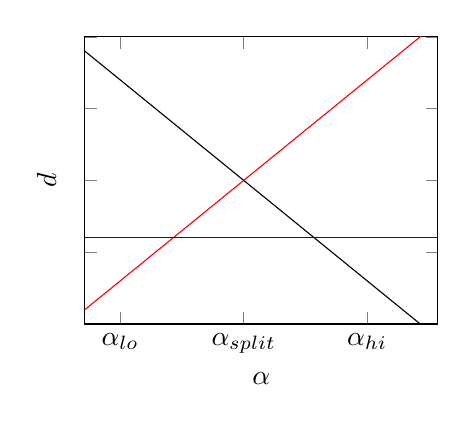
\begin{tikzpicture}
        \begin{axis}[ 
        xlabel=$\alpha$,
        ylabel={$d$},
        xmin=0.4,
        xmax=0.9,
        xtick={0.45,0.625,0.8},
        xticklabels={$\alpha_{lo}$, $\alpha_{split}$, $\alpha_{hi}$},
        width=0.5\textwidth,
        yticklabels={,,}
        ] 
        \addplot[mark=none, red] {-3+8*x}; 
        \addplot[mark=none, black] {-8*x+7};
        \addplot[mark=none, blue] {1.2};
        \end{axis} 
    \end{tikzpicture}
    \caption{Simply calculating the split values between the start and the end value of the range $[\alpha_{lo}, \alpha_{hi}]$ will not necessarily lead to the optimal values. By doing so, the blue line (constant $d$ value) will not be considered.}
    \label{fig:notoptimal}
\end{figure}

In order to solve this, we can recursively check each resulting interval again if it contains different merging behaviors.

\begin{figure}[h]
    \centering
    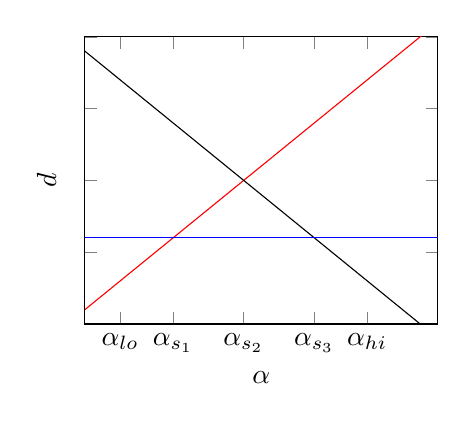
\begin{tikzpicture}
        \begin{axis}[ 
        xlabel=$\alpha$,
        ylabel={$d$},
        xmin=0.4,
        xmax=0.9,
        xtick={0.45,0.525,0.625,0.725,0.8},
        xticklabels={$\alpha_{lo}$, $\alpha_{s_1}$, $\alpha_{s_2}$, $\alpha_{s_3}$, $\alpha_{hi}$},
        width=0.5\textwidth,
        yticklabels={,,}
        ] 
        \addplot[mark=none, red] {-3+8*x}; 
        \addplot[mark=none, black] {-8*x+7};
        \addplot[mark=none, blue] {1.2};
        \end{axis} 
    \end{tikzpicture}
    \caption{Simply calculating the split values between the start and the end value of the range $[\alpha_{lo}, \alpha_{hi}]$ will not necessarily lead to the optimal values. By doing so, the blue line (constant $d$ value) will not be considered.}
    \label{fig:notoptimal2}
\end{figure}

By calculating the split points recursively, the example in figure \ref{fig:notoptimal2} will result in the intervals $[\alpha_{lo}, \alpha_{s_1}]$, $[\alpha_{s_1}, \alpha_{s_2}]$, $[\alpha_{s_2}, \alpha_{s_3}]$ and $[\alpha_{s_3}, \alpha_{s_{hi}}]$. The optimal distance between $\alpha_{s_1}$ and $\alpha_{s_3}$ is covered now, but the results contain one unncessary interval as $\alpha_{s_2}$ still splits two intervals. The algorithm can check if older splits are still relevant, however the runtime cost to do so will be more expensive than carrying one additional interval with the same distance. We can use this knowledge and adapt algorithm \ref{alg:alphalinkage1}.

\begin{algorithm}[H]
    \KwData{input data $p_1, ..., p_N$, initial states $st$}
    \KwResult{$k$ intervals $[\alpha_0, \alpha_1], ..., [\alpha_{k-1},\alpha_k]$}
    \For{$iteration\gets1$ \KwTo $N-1$}{
        \ForEach{state $s \in st$}{%
        remove state $s$\;
        ranges $\gets$ find ranges between $s.\alpha_{lo}$ and $s.\alpha_{hi}$\;
        \ForEach{range $r \in ranges$}{%
                $cand \gets$ candidate for range\;
                $ms \gets$ merge $cand$\;
                add state $ms$ with range $r$ to the end of $st$\;
        }
      }
    }
    \caption{By calculating the split points between $\alpha_{lo}$ and $\alpha_{hi}$ recursively, we ensure that no optimal interval is left out.}
    \label{alg:alphalinkage2}
\end{algorithm}

As experimental results turn out to need a lot of memory (up to $\approx$ 20 GB for 300 points and 20,000 states), we want to adapt algorithm \ref{alg:alphalinkage2} so that it uses less memory. The memory usage scales relative to the amount of currently in-memory stored states, so the goal is to reduce these. As the amount of states is much larger than the amound of iterations, we calculate and evaluate the leave nodes of the tree and keep the alternative merges stored. This results in algorithm \ref{alg:alphalinkage3}.

\begin{algorithm}[H]
    \KwData{input data $p_1, ..., p_N$, initial states $st$}
    \KwResult{$k$ intervals $[\alpha_0, \alpha_1], ..., [\alpha_{k-1},\alpha_k]$}
    \While{$\|st\| > 0$}{
        \ForEach{state $s \in st$}{%
        remove state $s$\;
        \eIf{$s$ is final}{
          evaluate $s$\;
          }{
          ranges $\gets$ find ranges between $s.\alpha_{lo}$ and $s.\alpha_{hi}$\;
            \ForEach{range $r \in ranges$}{%
                    $cand \gets$ candidate for range\;
                    $ms \gets$ merge $cand$\;
                    add state $ms$ with range $r$ to the beginning of $st$\;
            }
         }
      }
    }
    \caption{Instead of calculating the nodes layerwise, this algorithm works pathwise, i.e. it goes down one path of a tree to a leaf node and evaluates it before continuing with the next split. This approach needs much less memory than the previous algorithms and has about the same runtime as shown in figure \ref{fig:performance}.}
    \label{alg:alphalinkage3}
\end{algorithm}

\begin{figure}[h]
\centering
\begin{minipage}{.45\textwidth}
  \centering
  \includegraphics[width=\linewidth]{images/memory_mnist_ac}
\end{minipage}\hfill
\begin{minipage}{.45\textwidth}
  \centering
  \includegraphics[width=\linewidth]{images/runtime_mnist_ac}
\end{minipage}
\caption{The depth first implementation needs less memory and also has a better runtime compared to the breadth first implementation.}
\label{fig:performance}
\end{figure}

Instead of merging iteratively and steadily shrinking the intervals, we propose an algorithm with a geometric motivation. We are again evaluating an interval $[\alpha_{lo}, \alpha_{hi}]$, but we interprete the different merges as linear functions depending on $\alpha$. We can start by calculating the merge candidate for the start value $\alpha_{lo}$ and calculate the next intersection that will yield to the next merge. By calculating all the intersections of linear functions, we can also determine all the different intervals for the range $[\alpha_{lo}, \alpha_{hi}]$, where different merging behaviors occure. Algorithm \ref{alg:alphalinkage4} describes this procedure.

\begin{algorithm}[H]
    \KwData{input data $p_1, ..., p_N$, start value $\alpha_{lo}$, end value $\alpha_{hi}$}
    \KwResult{$k$ intervals $[\alpha_0, \alpha_1], ..., [\alpha_{k-1},\alpha_k]$}
    $\alpha \gets \alpha_{lo}$\;
    linear function $lf \gets$ get lf for alpha\;
    \While{$\alpha < \alpha_{hi}$}{
        $\alpha_{new} \gets$ calculate next split for $\alpha$\; 
        $lf \gets$ get lf for $\alpha_{new}$\;
        $\alpha \gets \alpha_{new}$
    }
    \caption{}
    \label{alg:alphalinkage4}
\end{algorithm}

\begin{figure}[h]
    \centering
    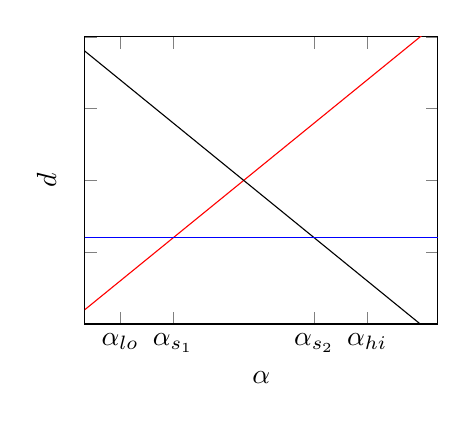
\begin{tikzpicture}
        \begin{axis}[ 
        xlabel=$\alpha$,
        ylabel={$d$},
        xmin=0.4,
        xmax=0.9,
        xtick={0.45,0.525,0.725,0.8},
        xticklabels={$\alpha_{lo}$, $\alpha_{s_1}$, $\alpha_{s_2}$, $\alpha_{hi}$},
        width=0.5\textwidth,
        yticklabels={,,}
        ] 
        \addplot[mark=none, red] {-3+8*x}; 
        \addplot[mark=none, black] {-8*x+7};
        \addplot[mark=none, blue] {1.2};
        \end{axis} 
    \end{tikzpicture}
    \caption{Simply calculating the split values between the start and the end value of the range $[\alpha_{lo}, \alpha_{hi}]$ will not necessarily lead to the optimal values. By doing so, the blue line (constant $d$ value) will not be considered.}
    \label{fig:optimal}
\end{figure}

\section{Performance Optimizations}

In order to have real-world applications, the proposed algorithms should run in an efficient way, i.e. it should not take the $\alpha$-linkage algorithms too much time to run. A first python implementation took days to run, but switching to C++ and using its advantages took down the runtime to hours. However, there are more optimization methods that we used in order to improve the runtime.

\subsection{Dynamic Programming}

One of the most time-consuming parts was the calculating of the distances. For each pair of clusters $C_i, C,j$ the distance had to be calculated for each clustering state. We optimized this by using dynamic programming and stored the distance matrices $D_{lower}$ and $D_{upper}$ for each state. The naming results from the different interpolation settings where we interpolate from one linkage distance (lower) to another linkage distance (upper), e.g. the setting in equation \ref{eq:singlecomplete} describes the interpolation from single linkage (lower) to complete linkage (upper). In this example we then store the pairwise distances for both single linkage and complete linkage and in order to find the merge candidates we have to do iterate over the distance matrices instead of calculating the distances over and over again. When we merge two clusters, we then update the distance matrices for the given state. Table \ref{dp:distances} shows an example for the pairwise distances of clusters $i$ and $j$.

\begin{table}[h]
    \centering
    \begin{tabular}{|l | l l l l l|}
    \hline
    j\textbackslash i & 0 & 1 & 2 & 3 & 4\\ \hline
    0 & 0 & 1.243 & 1.512 & 2.468 & 5.1243\\
    1 & 1.243 & 0 & 2.443 & 3.1412 & 4.443\\
    2 & 1.512 & 2.443 & 0 & 3.8988 & 6.827\\
    3 & 2.468 & 3.1412 & 3.8988 & 0 & 5.72\\
    4 & 5.1243 & 4.443 & 6.827 & 5.72 & 0\\ \hline
    \end{tabular}
    \caption{Storing the pairwise distances of all clusters avoids calculating the distances over and over again.}
    \label{dp:distances}
\end{table}

One observation that we can make is that the matrix has a lot of redundant values, because $D(i,j) = D(j,i)$. Removing these rendundant values will result in a trade-off between copying and indexing costs and will be discussed in the following section. Another optimization we can do is storing the indices of the active clusters, i.e. the clusters that can get merged. Once two clusters got merged, they cannot be merged any further, only the resulting cluster can. So we then do not have to consider the old clusters anymore and can remove them from the set of active indicies. This allows us to find the merge candidates faster as the pool of candidates gets smaller.

\subsection{Trade-Off between Copying and Indexing Costs}

Currently we can access the costs for a pair of clusters $C_i$ and $C_j$ through $D[i,j]$ or $D[i + j * width]$ for flattened matrices. These indices are very easy to calculate. In order to remove the redundant values from the distance matrix we remove all values below the diagonal as shown in table \ref{dp:distances2}.

\begin{table}[h]
    \centering
    \begin{tabular}{|l | l l l l l|}
    \hline
    j\textbackslash i & 0 & 1 & 2 & 3 & 4\\ \hline
    0 & 0 & 1.243 & 1.512 & 2.468 & 5.1243\\
    1 & & 0 & 2.443 & 3.1412 & 4.443\\
    2 & & & 0 & 3.8988 & 6.827\\
    3 & & & & 0 & 5.72\\
    4 & & & & & 0\\ \hline
    \end{tabular}
    \caption{Storing the pairwise distances of all clusters avoids calculating the distances over and over again.}
    \label{dp:distances2}
\end{table}

In addition to that we can also remove the diagonal values as they represent the distances between the same clusters and are thus always zero. This results in table \ref{dp:distances3}.

\begin{table}[h]
    \centering
    \begin{tabular}{|l | l l l l l|}
    \hline
    j\textbackslash i & 0 & 1 & 2 & 3 & 4\\ \hline
    0 & & 1.243 & 1.512 & 2.468 & 5.1243\\
    1 & & & 2.443 & 3.1412 & 4.443\\
    2 & & & & 3.8988 & 6.827\\
    3 & & & & & 5.72\\
    4 & & & & &\\ \hline
    \end{tabular}
    \caption{Storing the pairwise distances of all clusters avoids calculating the distances over and over again.}
    \label{dp:distances3}
\end{table}

The matrices are now smaller, so they need less memory. In the example, we changed a matrix of the size $25$ to a matrix of the size $10$. In general a matrix of the size $n$x$n$ will be compressed to a matrix of the size $\frac{n^2-n}{2}$. The lower amount of needed memory also results in less copying costs that will lead to a better runtime. However, the indexing is not as easy anymore. For easier storage, we again work with flattened matrices, the indexing for the resulting list is shown in equation \ref{eq:indexing}.

\begin{equation}
    \begin{aligned}
        index(i,j) = \frac{width * (width - 1)}{2} - \frac{(width - j) * (width - j - 1)}{2} + i - j - 1
    \end{aligned}
    \label{eq:indexing}
\end{equation}

Calculating this index in a nested loop is very expensive, however we calculate the part that does not depend on $i$ in the outer loop and thus only need to add $i$ in the inner loop. This does not only yield to a lower memory usage of $\approx 30\%$, but also increases the runtime by TODO.

\subsection{Implementation-specific Optimizations}

In order to optimize the implementation even further, we will have a look into the implementation. One optimization that already was briefly described is the flatterning of the matrices, so the resulting list will be one-dimensional and can be iterated easier and faster.

Another observation is that copy operations are computationally expensive, so we avoid them as much as possible. In the described algorithms (\ref{alg:alphalinkage1}, \ref{alg:alphalinkage2} and \ref{alg:alphalinkage3}) we removed a state from the list of states and added other states. In an optimized way, we do not remove the state and just overwrite the state with the resulting state. Once there are splits in the current interval, the state gets overwritten and additional states get added to the list.

We can also optimize the way of updating the distance matrices. Instead of adding new clusters there for a merge of clusters $i$ and $j$ we update the distances of $i$ to all active clusters with the distances of the resulting cluster. The distances of the cluster $j$ will not be considered for merges anymore as the index $j$ gets removed from the active indices. This has the advantage that the size of the distance matrices will not increase after merges.

Also, the data types make an important contribution to the memory usage. Instead of using double precision floating point values, single precision is enough to clearly identify and separate all the resulting intervals. Same goes for the distances as we only need the minimum and maximum distances, that are not effected by loss of precision. To store the indices of the clusters, we know that they will not exceed $2^{16}$, so they can be store as half precision values.

% \chapter{Optimizing the Metric}
\label{sec:beta}

In a similar fashion as described in section \ref{chapter:alphalinkage} this sections aims to optimize a metric that is a linear combination of several metrics. For instance, images can have a 2D pixel representation and a text describing the each image. Combining these features for clustering tasks can be problematic as it is not how the optimal weight between these features should be. Does a word describe more than a subset of the image, are the features equally important or does the pixel image lead to better clusterings? With $\beta$-linkage we provide a framework based on $\alpha$-linkage that calculates different merges based on linear combinations of representations and leads to optimized clusterings.

\begin{figure}[h]
    \centering
    \includegraphics[width=0.7\textwidth]{images/ExampleDataset}
    \caption{Combining several metrics seems often natural and can lead to improved results as in this example where we project a dataset on both axes.}
    \label{fig:metrics}
\end{figure}

For instance, figure \ref{fig:metrics} shows a set of points that might be put in clusters easily. However, if you only look at the distance regarding the $X_1$-axis or the $X_2$-axis clustering will be very difficult, because each of the axis does not describe the spatial correlation anymore. This example is selected on purpose to motivate the following experiments where we learn optimal combinations of different metrics.\\ 

To interpolate between $d_0$ and $d_1$, we use the same interpolation as discussed in section \ref{chapter:alphalinkage}. We use a parameter $\beta \in [0,1]$ and weight the metrics as shown in equation \ref{eq:betalinkage}.

\begin{equation}
d_\beta(x,x') = (1 - \beta) \cdot d_0(x,x') + \beta \cdot d_1(x,x')
\label{eq:betalinkage}
\end{equation}

\begin{equation}
d_\beta(x,x') = d_0(x,x') + \beta \cdot (d_1(x,x') - d_0(x,x'))
\label{eq:betalinear}
\end{equation}

We can then compete all possible discontinuities by comparing the distances of given clusters $(x, x')$ and $(y, y')$. As $d_\beta(x,x')$ is a linear function depending on $\beta$ (see equation \ref{eq:betalinear}), we can compute all discontinuities by solving the following equation.

\begin{align*}
&d_\beta(x,x') = d_\beta(y,y')\\
&(1 - \beta) \cdot d_0(x,x') + \beta \cdot d_1(x,x') = (1 - \beta) \cdot d_0(y,y') + \beta \cdot d_1(y,y')\\
&d_0(x,x') - \beta \cdot d_0(x,x')  + \beta \cdot d_1(x,x') = d_0(y,y') - \beta \cdot d_0(y,y') + \beta \cdot d_1(y,y')\\
&\beta \cdot (- d_0(x,x') + d_1(x,x') + d_0(y,y') - d_1(y,y')) = - d_0(x,x') + d_0(y,y')\\
&\beta = \frac{- d_0(x,x') + d_0(y,y')}{- d_0(x,x') + d_1(x,x') + d_0(y,y') - d_1(y,y')}
\label{eq:discont}
\end{align*}

As we know that the function $d_\beta$ is a linear function depending on $\beta$ and we showed that all discontinuities depend on four points, we know that there at most $O(n^4)$ well-defined intervals $I_i \in [0,1]$ for any clustering instance $S$, i.e. in any interval $I_i$ the algorithm will merge the same two points.

\todo[inline]{more details / explanations}

% % \chapter{$\alpha$-$\beta$-Linkage}

\section{Bilinear Interpolation between three different linkage strategies}

\section{Adapted Algorithm}

% \chapter{Experimental Setup}
\label{chapter:setup}

This work evaluates the proposed algorithms for image and text data. This chapter describes the used datasets and evaluation methods.

\section{Data Sets}
\label{chapter:datasets}

\subsection{Synthetic Data}

To motivate our approach, we manually created a dataset containing disks and rings as shown in figure \ref{fig:disksrings}. In this case, we know that single linkage performs well clustering the two rings, however it might be problematic to cluster the disks. On the other hand, complete linkage is expected to cluster the disks very well, but it might connect the two rings earlier than wanted. This data motivates our approach of interpolating between different linkage strategies, however the data is not natural and real-world datasets are very likely to have a different structure. 

\begin{figure}[h]
    \centering
    \includegraphics[width=0.7\textwidth]{images/RingsDisks}
    \caption{We use disks and rings as a sample dataset to motivate our $\alpha$-linkage approach. The dataset contains four clusters, two disks and two rings.}
    \label{fig:disksrings}
\end{figure}

\subsection{Text Data}

\paragraph{Never-Ending Language Learner data.} The Never-Ending Language Learner (NELL) is a learning agent that reads the web, extracts data and verifies beliefs \cite{Mitchell:2015:NL:2886521.2886641, Mitchell:2018:NL:3210350.3191513}. NELL, for example, knows that "Pittsburgh" is located in "Pennsylvania". These beliefs represent different noun-phrases such as "Pittsburgh" and "Pennsylvania". The noun-phrases belong to certain categories, e.g.``Pittsburg'' is a ``City'' and ``Pennsylvania'' is a ``State''. These subcategories both belong to the main category "Geopolitical Location". Figure \ref{fig:nell_beliefs} shows such a knowledge graph. While there are already different subcategories, the goal for a hierarchical clustering algorithm here could be to extract new useful subcategories.

\begin{figure}[h]
    \centering
    \includegraphics[width=0.7\textwidth]{images/nell_beliefs}
    \caption{The Never-Ending Language Learner represents different entities and their correlations \cite{Mitchell:2018:NL:3210350.3191513}.}
    \label{fig:nell_beliefs}
\end{figure}

The used dataset, extracted web-information by NELL, contains 32 different main categories, such as "Animal", "Location" or "Person". We limit each of these categories up to 250 and 1000 different entities that belong to different subcategories, so we can run experiments with 250 points and later on with 1000 points. Exemplary entities for the category "Animal" are "Otter", "Squirrel" or "Wolf". 
\newpage
\subsection{Image Data}

\paragraph{MNIST handwritten digits.} The MNIST handwritten digit database contains images of the handwritten digits from zero to nine \cite{lecun-mnisthandwrittendigit-2010}. Samples of these images are shown in figure \ref{fig:mnist}. Its training set contains a total of 60,000 images, where each image is represented as a 784-dimensional vector corresponding to an image with $28 \times 28$ black and white pixels.

\begin{figure}[h]
    \centering
    \includegraphics[width=0.7\textwidth]{images/mnist}
    \caption{The MNIST handwritten digits database contains 60,000 black and white images of handwritten digits ranging from zero to nine. These samples show ten randomly drawn samples for each label represented as a $28 \times 28$ pixel image \cite{lecun-mnisthandwrittendigit-2010}.}
    \label{fig:mnist}
\end{figure}

The goal of clustering MNIST images is to find an unsupervised learning method that can distinguish between black and white images. In addition, we can define various clustering tasks where we pick a subsample of the ten labels and then try to transfer the results to other subsamples. For example, we first cluster images labeled as zero, one, two, three or four and later apply the gained knowledge for clustering images labeled as five, six, seven, eight or nine. These types of experiments allow high-level transfer learning if we define several different clustering tasks, e.g. for five different labels there are $10 \choose 5$ $= 252$ different combinations of labels.\\

Another observation that results from hierarchical clustering is the similarity of different labels, i.e. which labels are likely to get clustered together. For instance, we would expect images of characters 6 and 9, 3 and 8 or 2 and 5 to have some attributes in common and thus get clustered together rather than with other digits.

\paragraph{CIFAR-10.} Another image dataset this thesis uses for evaluation is the CIFAR-10 dataset that contains 60,000 RGB images of ten different categories \cite{Krizhevsky2009LearningML}. Each image consists of $32 \times 32$ pixels and is thus represented as a 3072-dimensional vector ($32 \times 32 \times 3$). The categories and ten random images from each are shown in figure \ref{fig:cifar10}.

\begin{figure}[h]
    \centering
    \includegraphics[width=0.7\textwidth]{images/cifar10}
    \caption{The CIFAR-10 database contains 60,000 RGB images of the ten shown different classes. These samples show ten randomly drawn samples for each label represented as a $32 \times 32$ pixel image \cite{Krizhevsky2009LearningML}.}
    \label{fig:cifar10}
\end{figure}

As the amount of images and the amount of classes is equal to the ones in the MNIST dataset, we can also try similar experiments. The main difference is that the images consist of RGB pixels instead of black and white pixel values.

\paragraph{CIFAR-100.} The CIFAR-100 dataset contains similar images, but instead of 6,000 images each for 10 classes, it consists of 600 images for each of 100 classes. The classes are divided into 20 superclasses each containing five subclasses. Examples of superclasses and corresponding subclasses are shown in table \ref{table:cifar100data}. 

\begin{table}[h]
    \centering
    \begin{tabular}{|l|l|}
    \hline
    superclass      & subclasses                                  \\ \hline
    aquatic mammals & beaver, dolphin, otter, seal, whale         \\
    fish            & aquarium fish, flatfish, ray, shark, trout  \\
    flowers         & orchids, poppies, roses, sunflowers, tulips \\
    people          & baby, boy, girl, man, woman                 \\ 
    reptiles        & crocodile, dinosaur, lizard, snake, turtle  \\ \hline               
    \end{tabular}
    \caption{The CIFAR-100 dataset contains 20 different superclasses, each with five different subclasses leading to 100 classes overall. The images are represented in the same way as in the CIFAR-10 dataset, i.e. by a 3072-dimensional vector \cite{Krizhevsky2009LearningML}.}
    \label{table:cifar100data}
\end{table}

Having superclasses and subclasses allows clustering between different subclasses within a superclass and also between different superclasses. This allows more experiments than for the CIFAR10 data.

\paragraph{Omniglot.}The Omniglot dataset contains 1623 handwritten characters from 30 different alphabets, where each character is represented by 20 different images. Each image is black and white and represented by $105 \times 105$ pixels \cite{Lake1332}. Figure \ref{fig:omniglotcharacters} shows characters of the more well-known Latin, Greek and Hebrew alphabets that are included in the dataset together with less known alphabets such as Tagalog, a language spoken as a first language by 25\% of the population of the Philippines.

\begin{figure}[h]
\centering
\begin{minipage}{.32\textwidth}
  \centering
  \includegraphics[width=\linewidth]{images/latin}
\end{minipage}
\begin{minipage}{.32\textwidth}
  \centering
  \includegraphics[width=\linewidth]{images/greek}
\end{minipage}
\begin{minipage}{.32\textwidth}
  \centering
  \includegraphics[width=\linewidth]{images/hebrew}
\end{minipage}
\caption{The Omniglot dataset contains handwritten characters of different alphabets, such as Latin (left), Greek (middle) and Hebrew (right) \cite{Lake1332}.}
\label{fig:omniglotcharacters}
\end{figure}

The Omniglot dataset is similar to the MNIST dataset as it also contains handwritten characters, however it has more different characters and fewer images for each of the characters. This allows us to run more learning tasks. In addition, the dataset also contains stroke data of each of the images, i.e.\ the time series data of the actual drawings where each observation corresponds to a (x,y)-coordinate together with a timestamp. This gives us insight into the order in which the character was written. Figure \ref{fig:omniglotstroke} shows an example of strokes for one character of the Tagalog alphabet.

\begin{figure}[h]
  \centering
  \includegraphics[width=.6\textwidth]{plots/demo_strokes}
  \caption{The stroke data gives a time series representation of the Omniglot drawings that indicate in which order the characters were written \cite{Lake1332}.}
  \label{fig:omniglotstroke}
\end{figure}

\section{Pruning}

In order to evaluate a cluster tree together with the target labels, we have to prune the tree into the corresponding number of $k$ target clusters, i.e.\ the $k$ different classes of the target data. Therefore, we evaluate the costs of all possible combinations of $k$ clusters and select the best clusters. Figure \ref{fig:pruning} shows an example of how we can prune a cluster tree into $k = 3$ clusters by either using the clusters $C, D$ and $E$ or the clusters $B, F$ and $G$.

\begin{figure}[h]
\centering
\begin{minipage}{.45\textwidth}
  \centering
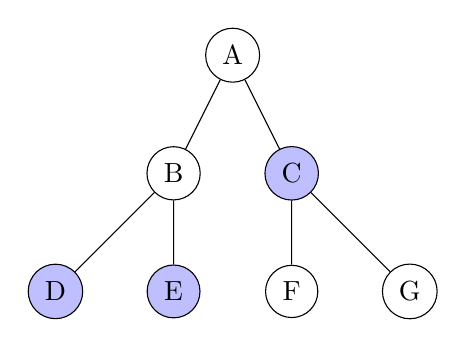
\begin{tikzpicture}
 
\node[circle,draw]{A}
	child { node[circle,draw] {B}
    child { node[circle,draw,fill=blue, fill opacity=0.25,text opacity=1] {D}}
	  child { node[circle,draw,fill=blue, fill opacity=0.25,text opacity=1] {E}}
    child[missing]{}
  }
	child { node[circle,draw,fill=blue, fill opacity=0.25,text opacity=1] {C}
    child[missing]{}
    child { node[circle,draw] {F}}
	  child { node[circle,draw] {G}}
  }
;
\end{tikzpicture}
\end{minipage}
\begin{minipage}{.45\textwidth}
  \centering
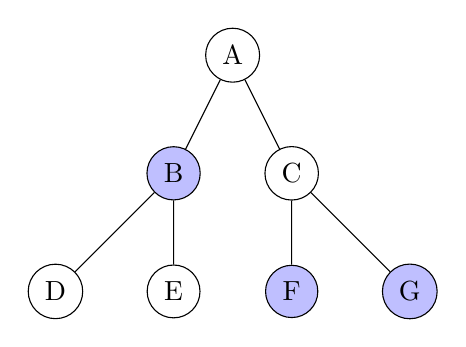
\begin{tikzpicture}
 
\node[circle,draw]{A}
	child { node[circle,draw,fill=blue, fill opacity=0.25,text opacity=1] {B}
    child { node[circle,draw] {D}}
	  child { node[circle,draw] {E}}
    child[missing]{}
  }
	child { node[circle,draw] {C}
    child[missing]{}
    child { node[circle,draw,fill=blue, fill opacity=0.25,text opacity=1] {F}}
	  child { node[circle,draw,fill=blue, fill opacity=0.25,text opacity=1] {G}}
  }
;
\end{tikzpicture}
\end{minipage}
\caption{There are multiple ways we can prune a cluster tree into $k$ clusters.}
\label{fig:pruning}
\end{figure}

However, we still have to find a way to calculate the preferred pruning of a cluster tree into $k$ clusters, i.e.\ whether in case of figure \ref{fig:pruning} we would prefer the pruning on the left or the one on the right.

\section{Cost functions}
\label{chapter:costfunctions}

In order to evaluate the quality of a clustering, we need some kind of cost function that compares the generated clustering $C_1,...,C_k$ with the target clustering $C_1^*, ..., C_k^*$ and calculates a quality score indicating how good they match. 

\paragraph{Majority Cost.} One method to compare them is the Majority distance as shown in equation \ref{eq:majoritydistance} where $n$ is the number of sampled points.

\begin{equation}
    \begin{aligned}
        cost_{Majority}(C_{1:k}, C_{1:k}^*) = \frac{1}{n} \sum_{i=1}^k \min_{j \in [m]} |C_i - C'_j|
    \end{aligned}
    \label{eq:majoritydistance}
\end{equation}

This cost function is motivated by finding corresponding clusters with the lowest distance, i.e. each generated cluster gets matched with the optimal target cluster and the cost is the average difference between the matched cluster pairs. However, two generated clusters can be matched with the same target cluster. 

\paragraph{Hamming Cost.} This motivates the Hamming distance as shown in figure \ref{eq:hammingdistance}. We denote $\mathbb{S}_k$ as all possible permutations of the $k$ clusters.

\begin{equation}
    \begin{aligned}
        cost_{Hamming}(C_{1:k}, C'_{1:k}) = \frac{1}{n} \min_{\sigma \in \mathbb{S}_k} \sum_{i=1}^k |C_i - C'_{\sigma_i}|
    \end{aligned}
    \label{eq:hammingdistance}
\end{equation}

However, the Hamming distance contains an assignment problem to find the optimal matching $\sigma$ between the generated clusters and the target clusters. Table \ref{table:matching} shows how such a matching can look like.

\begin{table}[h]
    \centering
    \begin{tabular}{|l | l l l l l|}
    \hline
    j\textbackslash i & 1 & 2 & 3 & 4 & 5\\ \hline
    1 & 20 & \cellcolor{blue!25}15 & 30 & 50 & 40\\
    2 & 80 & 10 & \cellcolor{blue!25}15 & 20 & 30\\
    3 & \cellcolor{blue!25}20 & 30 & 50 & 80 & 60\\
    4 & 30 & 50 & 40 & \cellcolor{blue!25}20 & 10\\
    5 & 20 & 30 & 40 & 50 & \cellcolor{blue!25}25\\ \hline
    \end{tabular}
    \caption{In order to calculate the Hamming distance between two clusterings, we have to calculate the optimal mapping that results in the lowest distance for these two clusterings. For distances between clusterings $C_1^i, ..., C_k^i$ and $C_1^j, ..., C_k^j$ we can calculate the optimal mapping (highlighted cells) in a brute force way or more efficiently with the Hungarian method \cite{kuhn1955hungarian, munkres1957algorithms}.}
    \label{table:matching}
\end{table}

While solving the assignment with a brute force strategy would result in $O(n!)$ complexity, Harold Kuhn introduced the Hungarian method to solve the problem in $O(n^4)$ complexity \cite{kuhn1955hungarian}. Later on, James Munkres modified the algorithm to $O(n^3)$ complexity \cite{munkres1957algorithms}. In general, we can say that it  makes sense to use the Hungarian method when there are more than five target classes. A detailed explanation of the Hungarian method is included in Appendix \ref{sec:hungarian}.

\section{Parameter Advising}

Our settings average over multiple experiments and show one parameter $\alpha$ that represents the best clustering over all experiments, i.e. the algorithm automatically outputs the best result. For parameter advising, we select the top $k$ values of $\alpha$ for each experiment and calculate the clustering's cost with the best of the $k$ values of $\alpha$ \cite{deblasio2015parameter}. We select the pool of $\alpha$-values through the local optima for each of the $n$ experiments. The best $k$ values of $\alpha$, where $k << n$, can then be calculated with an integer optimization problem. A possible scenario where this setup is useful is by having a domain expert, who can select the best from $k$ suggested clusterings.\\

More formally, we want to to find the optimal parameters $\alpha_1^*, \dots, \alpha_k^*$ such that they optimize the utility $u$ of a clustering instance $S$ and the resulting cluster tree $T(S, \alpha)$ (see equation \ref{eq:advising}). In order to calculate the parameters $\alpha_1^*, \dots, \alpha_k^*$, we first have a look at parameter advising described as a facility location problem.

\begin{equation}
  \alpha_1^*, \dots, \alpha_k^*
  = \argmax_{\alpha_1, \dots, \alpha_k} \sum_{i=1}^N \max_{j \in [k]} u\bigl(S, T(S, \alpha_j)\bigr).
  \label{eq:advising}
\end{equation}

\paragraph{Facility Location Advising.} We create an integer optimization problem for a candidate set $\alpha_1, \dots, \alpha_m$ over the clustering instances $S_1, \dots, S_N$ and introduce the selection parameters $y_1, \dots, y_m \in \{0, 1\}$ that indicate whether $\alpha_j$ is used as one of the $k$ parameters. Also, we denote $x_{ij} \in \{0, 1\}$ as the auxiliary variable with the interpretation that $x_{ij} = 1$ whenever $\alpha_j$ is the best chosen parameter for problem instance $S_i$. This leads to the following optimization problem that maximizes the overall utility.

\begin{align*}
  \argmax_{x_{ij}, y_j} \qquad&\sum_{i = 1}^N \sum_{j = 1}^m x_{ij} u(S_i, T(S_i, \alpha_j)) \\
  \text{subject to} \qquad& \sum_{j=1}^m y_j = k \\
  & \text{for each $i \in [N]$, } \sum_{j=1}^m x_{ij} = 1 \\
  & \text{for each $i \in [N], j \in [M]$, } x_{ij} \leq y_j.
\end{align*}

Note that the optimization problem contains three constraints. $\sum_{j=1}^m y_j = k$ makes sure that exactly $k$ values are used, the second guarantees that we assign any clustering instance to at most one parameter, and the final constraint ensures that we only assign clustering instances to selected parameters. In our experiments, we use IBM ILOG CPLEX to solve these integer programming problems. However, the computation of the optimal values is very complex, so we also implement a greedy strategy that calculates approximately optimal values more efficiently.

\paragraph{Greedy Parameter Advising.} In a convex space, an optimal value $\alpha_n^*$ will also be optimal when calculating $k = n + 1$ optimal values. Leveraging this knowledge, we can iteratively calculate the optimal values $\alpha_1, \dots, \alpha_m$ step by step, where we first calculate $\alpha_1^*$ that has the largest utility over all clustering instances $S$ and then calculate $\alpha_2^*$ that results in the highest utility combined with $\alpha_1^*$ (see equation \ref{eq:greedypa}).

\begin{equation}
\sum_{i=1}^N \max\{u(S_i, T(S_i, \alpha_1)), u(S_i, T(S_i, \alpha_2)\} 
\label{eq:greedypa}
\end{equation}

The results of the experiments with the mentioned datasets are discussed in the following section \ref{sec:results}. % Experimental Setup

% \chapter{Results and Discussion}
\label{sec:results}

We evaluated the in chapter \ref{chapter:alphalinkage} proposed algorithms with the in chapter \ref{chapter:datasets} discussed datasets aiming to find new subcategories for the text data and to generate better clusterings overall. The quality of the clusterings was calculated with the in chapter \ref{chapter:costfunctions} explained cost functions.

\section{Clustering Text Data}

We subsampled the NELL data to a maximum of 250 points in each class and then evaluated each of the 32 classes separately. Figure \ref{fig:nellresults} shows the resulting majority distances for the three different types of linear interpolation.

\begin{figure}[h]
\centering
\begin{minipage}{.3\textwidth}
  \centering
  \includegraphics[width=\linewidth]{images/nell_sc}
\end{minipage}
\begin{minipage}{.3\textwidth}
  \centering
  \includegraphics[width=\linewidth]{images/nell_sa}
\end{minipage}
\begin{minipage}{.3\textwidth}
  \centering
  \includegraphics[width=\linewidth]{images/nell_ac}
\end{minipage}
\caption{The omniglot dataset contains handwritten characters of different alphabets, such as Latin, Greek and Hebrew \cite{Lake1332}.}
\label{fig:nellresults}
\end{figure}

We observe that single linkage performs very poorly and complete linkage performs very well for the NELL data. Table \ref{table:nellresults} shows the improvements we got over the other clustering strategies.

\begin{table}[h]
    \centering
    \begin{tabular}{|l | l|}
    \hline
    Strategy & Majority Cost\\ \hline
    Single Linkage & 0.36871\\
    Average Linkage & 0.248913\\
    Complete Linkage & 0.15935\\
    $\alpha_{SC}(0.825)$ & 0.15442\\
    $\alpha_{AC}(0.825)$ & 0.15569\\\hline
    \end{tabular}
    \caption{Our proposed algorithm reduces the cost by $\Delta cost = 0.493\%$.}
    \label{table:nellresults}
\end{table}

The total improvement over the common linkage methods is $0.493\%$ and the best clustering we generated had an error of $15.442\%$. With this clustering we also managed to extract new subcategories as listed in table \ref{table:nellcategories}.

In addition to averaged costs, we also evaluated the clusterings for multiple values of $\alpha$. This is helpful in situations where a domain expert can select from multiple suggestions. For example, if we consider the best three values of $\alpha$, the domain expert can choose from three different clusterings. In order to calculate the $N$ best values of $\alpha$, we selected the 32 optimal values resulting from the experiments that led to an integer optimization problem. This resulted in ?????.

As our only formal guarantee was that there will be a maximum of $O(n^8)$ intervals in the range between single and complete linkage, we also had a look at the actual results. Since the proof for single and complete linkage in Balcan et. al \cite{DBLP:journals/corr/BalcanNVW16} relies on the fact that the distance $d_{SC}(X,Y,\alpha)$ is based on four points and a split between two merges thus is based on eight points, we would expect experiments containing average linkage to have more intervals, because the average linkage distance is based on all points of the clusters. Finding formal guarantees for the average distance is not a part of this thesis and will briefly be discussed in section \ref{section:futurework}.

\section{Clustering Image Data}

We first clustered the MNIST data. First experiments were run with 250 points in each run.

\begin{figure}[h]
\centering
\begin{minipage}{.3\textwidth}
  \centering
  \includegraphics[width=\linewidth]{images/MNIST_SC_250}
\end{minipage}
\begin{minipage}{.3\textwidth}
  \centering
  \includegraphics[width=\linewidth]{images/MNIST_SA_250}
\end{minipage}
\begin{minipage}{.3\textwidth}
  \centering
  \includegraphics[width=\linewidth]{images/MNIST_AC_250}
\end{minipage}
\caption{The omniglot dataset contains handwritten characters of different alphabets, such as Latin, Greek and Hebrew \cite{Lake1332}.}
\label{fig:mnist250}
\end{figure}

Figure \ref{fig:mnist250} shows the experimental results averaged over all 252 $10 \choose 5$ experiments, i.e. all different combinations of five unique labels. Again, we observe that interpolating between single and average linkage does not give us good results. Table \ref{table:mnist250results} summarizes the results we obtain for these experiments.

\begin{table}[h]
    \centering
    \begin{tabular}{|l | l|}
    \hline
    Strategy & Hamming Cost\\ \hline
    Single Linkage & 0.782354\\
    Average Linkage & 0.634206\\
    Complete Linkage & 0.441931\\
    $\alpha_{SC}(0.861624,)$ & 0.420714\\
    $\alpha_{AC}(0.849407)$ & 0.416627\\\hline
    \end{tabular}
    \caption{Our proposed algorithm reduces the cost by $\Delta cost = 2.5304\%$.}
    \label{table:mnist250results}
\end{table}

Reducing the cost by $\Delta cost = 2.5304\%$ seems to be a good result already. However the goal was to learn a parameter $\alpha$ that represents the entire dataset well. Because the procedure is very ressource-expensive, the results only looked at the first 500 points of the dataset as we clustered points from five labels in experiments of 250 points, i.e. we were using the first 50 points for each of the ten labels. This led us to running the same setting with other batches of the dataset to see if the subset of 500 points gives a good representation of the entire dataset. Figure ??? shows the results for the second batch and unfortunately the curves look quite differently, i.e. the batch did not give a good representation for the dataset.

To overcome this problem, we decided to scale up the experiments, so each of them used 1,000 instead of 250 points. As we used cloud computing to run the experiments in a reasonable time, we only evaluated the single to complete linkage and the average to complete linkage interpolation. We started with the single to complete linkage interpolation, where we show the results for the first six batches in figure \ref{fig:mnist1000sc}. Each batch contains 2,000 points, i.e. the six batches cover the first 12,000 points of the dataset.

\begin{figure}[h]
\centering
\begin{minipage}{.3\textwidth}
  \centering
  \includegraphics[width=\linewidth]{images/mnist-sc-0}
\end{minipage}
\begin{minipage}{.3\textwidth}
  \centering
  \includegraphics[width=\linewidth]{images/mnist-sc-1}
\end{minipage}
\begin{minipage}{.3\textwidth}
  \centering
  \includegraphics[width=\linewidth]{images/mnist-sc-2}
\end{minipage}
\begin{minipage}{.3\textwidth}
  \centering
  \includegraphics[width=\linewidth]{images/mnist-sc-3}
\end{minipage}
\begin{minipage}{.3\textwidth}
  \centering
  \includegraphics[width=\linewidth]{images/mnist-sc-4}
\end{minipage}
\begin{minipage}{.3\textwidth}
  \centering
  \includegraphics[width=\linewidth]{images/mnist-sc-5}
\end{minipage}
\caption{The first six batches of the MNIST dataset result in similar curves when being evaluated between single and complete linkage.}
\label{fig:mnist1000sc}
\end{figure}

As the curves look quite similar, we also want to analyse if the optimal values are similar. Thus we calculate the hamming cost for the optimal value of $\alpha$ in table \ref{table:mnist1000sc}.

\begin{table}[h]
    \centering
    \begin{tabular}{|l | l l l l l l |}
    \hline
    Strategy & Batch 0 & Batch 1 & Batch 2 & Batch 3 & Batch 4 & Batch 5\\ \hline
    Single Linkage & 0.796901 & 0.797345 & 0.797171 & 0.797405 & 0.796766 & 0.797024\\
    Complete Linkage & 0.490468 & 0.461063 & 0.479825 & 0.475329 & 0.463321 & 0.487111\\
    $\alpha_{opt}$ & 0.87228 & 0.84419 & 0.778498 & 0.83199 & 0.82338 & 0.852251\\
    $cost_{opt}$ & 0.450012 & 0.416433 & 0.431143 & 0.423786 & 0.421103 & 0.446032\\
    $\Delta cost$ & 4.0456\% & 4.463\% & 4.8682\% & 5.1543\% & 4.2218\% & 4.1079\%\\\hline
    \end{tabular}
    \caption{Our proposed algorithm reduces the cost by up to $\Delta_{max} cost = 5.1543\%$.}
    \label{table:mnist1000sc}
\end{table}

We were running the same experiments for the interpolation between average and complete linkage.

\begin{figure}[h]
\centering
\begin{minipage}{.3\textwidth}
  \centering
  \includegraphics[width=\linewidth]{images/mnist-ac-0}
\end{minipage}
\begin{minipage}{.3\textwidth}
  \centering
  \includegraphics[width=\linewidth]{images/mnist-ac-1}
\end{minipage}
\begin{minipage}{.3\textwidth}
  \centering
  \includegraphics[width=\linewidth]{images/mnist-ac-2}
\end{minipage}
\begin{minipage}{.3\textwidth}
  \centering
  \includegraphics[width=\linewidth]{images/mnist-ac-3}
\end{minipage}
\begin{minipage}{.3\textwidth}
  \centering
  \includegraphics[width=\linewidth]{images/mnist-ac-4}
\end{minipage}
\begin{minipage}{.3\textwidth}
  \centering
  \includegraphics[width=\linewidth]{images/mnist-ac-5}
\end{minipage}
\caption{The omniglot dataset contains handwritten characters of different alphabets, such as Latin, Greek and Hebrew \cite{Lake1332}.}
\label{fig:mnist1000ac}
\end{figure}

\begin{table}[h]
    \centering
    \begin{tabular}{|l | l l l l l l |}
    \hline
    Strategy & Batch 0 & Batch 1 & Batch 2 & Batch 3 & Batch 4 & Batch 5\\ \hline
    Average Linkage & 0.664952 & 0.672583 & 0.623325 & 0.679929 & 0.657857 & 0.652774\\
    Complete Linkage & 0.490468 & 0.461063 & 0.479825 & 0.475329 & 0.463321 & 0.487111\\
    $\alpha_{opt}$ & 0.7869 & 0.7124 & 0.634 & 0.807697 & 0.536073 & 0.5305\\
    $cost_{opt}$ & 0.458167 & 0.406563 & 0.440964 & 0.451063 & 0.429849 & 0.431631\\
    $\Delta cost$ & 3.2301\% & 5.45\% & 3.8861\% & 2.4266\% & 3.3472\% & 5.548\%\\\hline
    \end{tabular}
    \caption{Our proposed algorithm reduces the cost by up to $\Delta_{max} cost = 5.548\%$.}
    \label{table:mnist1000ac}
\end{table}

The curves for interpolating between average and complete linkage in figure \ref{ref:mnist1000ac} vary more than the curves for interpolating between single and complete linkage \ref{fig:mnist1000sc}. This results in a higher variation in the optimal values of $\alpha$ and the performance increase as shown in table \ref{table:mnist1000ac}.

In order to compare the both interpolation strategies, we averaged over the six batches to to see how well the different batches fit to each other. The results are shown in figure \ref{fig:mnist1000avg}.

\begin{figure}[h]
\centering
\begin{minipage}{.45\textwidth}
  \centering
  \includegraphics[width=\linewidth]{images/mnist-sc-averaged}
\end{minipage}
\begin{minipage}{.45\textwidth}
  \centering
  \includegraphics[width=\linewidth]{images/mnist-ac-averaged}
\end{minipage}
\caption{Averaging the first six batches over both linkage strategies allows us to see how good they perform on the first 12,000 points of the MNIST dataset.}
\label{fig:mnist1000avg}
\end{figure}

Figure \ref{fig:mnist1000avg} shows that both strategies give a valuable improvement over single, average and complete linkage on the first 12,000 points of the MNIST dataset. The exact improvement is shown in table \ref{table:mnist1000avg}.

\begin{table}[h]
    \centering
    \begin{tabular}{|l | l |}
    \hline
    Strategy & Hamming Cost\\ \hline
    Single Linkage & 0.797102\\
    Average Linkage & 0.65857\\
    Complete Linkage & 0.476186\\
    $cost_{opt_{SC}}$ & 0.439207\\
    $\Delta cost_{SC}$ & 3.6979\%\\
    $cost_{opt_{AC}}$ & 0.443139\\
    $\Delta cost_{AC}$ & 3.3047\%\\\hline
    \end{tabular}
    \caption{Our proposed algorithm reduces the cost by up to $\Delta_{max} cost = 5.548\%$.}
    \label{table:mnist1000avg}
\end{table}

Table \ref{table:mnist1000avg} shows that the improvement for average to complete linkage interpolation is $3.3\%$ and for single to complete linkage it is $3.7\%$. The optimal cost corresponds to $\alpha = 0.856557$ in the $SC$ setting and $\alpha = 0.63275$ in the $AC$ setting.

\begin{figure}[h]
\centering
\begin{minipage}{.45\textwidth}
  \centering
  \includegraphics[width=\linewidth]{images/mnist-sc-random}
\end{minipage}
\begin{minipage}{.45\textwidth}
  \centering
  \includegraphics[width=\linewidth]{images/mnist-ac-random}
\end{minipage}
\caption{The first six batches of the MNIST dataset result in similar curves when being evaluated between single and complete linkage.}
\label{fig:mnist1000sc}
\end{figure}

\section{Parameter Advising} % Results and Discussion

% \chapter{Conclusion}

In this work, we propose a data-driven solution to find the best algorithm, i.e.\ linkage strategy, for clustering tasks on a given dataset. In section \ref{chapter:alphalinkage} we introduce an algorithm to efficiently interpolate between the in section \ref{chapter:relatedwork} described linkage strategies. The final $\alpha$-linkage algorithm uses a sweep line approach to find the pairwise distance function that leads to merges with the lowest resulting cost, i.e.\ the optimal clusterings.\\

While the in section \ref{chapter:relatedwork} described approaches are less efficient, our approach is able to analyze large parts of the in section \ref{chapter:setup}  discussed real-world datasets using cloud computing. We summarize multiple key observations from the experiments in section \ref{sec:results}:
\begin{itemize}
\item Interpolating between single and complete linkage overcomes the hurdles of clustering data where both single and complete linkage perform better for some certain parts of the data. While single and complete linkage lead to an error of approximately $25\%$ for our synthetic data, in some experiments $\alpha$-linkage leads to optimal clusterings (i.e. an error of $0\%$).
\item For all our real-world datasets, we can sort the linkage strategies according to their quality in the following order (best first):
\begin{enumerate}
\item Complete Linkage
\item Average Linkage
\item Single Linkage
\end{enumerate}
\item Interpolating between single and average linkage does in general not lead to significant improvements.
\item When interpolating between single and complete or average and complete linkage, $\alpha$-linkage outperforms the used linkage strategies in all of our experiments with meaningful feature data.
\item Parameter Advising is a very powerful tool to provide more accurate clusterings. Our greedy implementation allows calculating the optimal parameters in an approximately optimal way very efficiently.
\end{itemize}

To be more precise, we show the results for the different datasets. In table \ref{table:comparison} we compare the single to complete linkage interpolation for all the discussed datasets\footnote{CIFAR-100 single to complete linkage was not discussed in this thesis.} in the batch setting. We notice that we achieve major improvements for all datasets and, excluding the synthetic data, receive similar values for $\alpha_{opt}$. This knowledge may be useful for transfer learning between different datasets in future work.

\begin{table}[H]
    \centering
    \begin{tabular}{|l | l | l | l | l | l |}
    \hline
    & Synthetic & NELL & MNIST & Omniglot & CIFAR-10\\ \hline
    $\alpha_{opt}$ & 0.169 & 0.918 & 0.857 & 0.908 & 0.917\\
    $\Delta_{cost}$ & 22.70\% & 1.20\% & 3.70\% & 1.0\% & 0.2\%\\\hline
    \end{tabular}
    \caption{Comparing the results over the different datasets while interpolating between single and complete linkage leads to similar parameters for many datasets.}
    \label{table:comparison}
\end{table}

Similar to table \ref{table:comparison}, we also show the results for interpolating between average and complete linkage in table \ref{table:comparison_ac}.

\begin{table}[H]
    \centering
    \begin{tabular}{|l | l | l | l | l | l | l |}
    \hline
    & Synthetic & NELL & MNIST & Omniglot & CIFAR-10 & CIFAR-100\\ \hline
    $\alpha_{opt}$ & 0.201 & 0.855 & 0.633 & 0.798 & 0.539 & 0.875\\
    $\Delta_{cost}$ & 0.29\% & 0.77\% & 3.30\% & 1.0\% & 0.83\% & 1.8\%\\\hline
    \end{tabular}
    \caption{Comparing the results over the different datasets while interpolating between average and complete linkage leads to a bigger spread of the parameters.}
    \label{table:comparison_ac}
\end{table}

In comparison to interpolating between single and complete linkage, we also obtain good improvements, however the optimal parameter $\alpha$ is spread more widely, i.e.\ it will be more difficult to reuse the gained knowledge for further use.\\

Also, we show in section \ref{sec:metric} that we can successfully apply the implemented framework to learning optimal metrics for given data as discussed in section \ref{sec:beta}. We achieve significant improvements by combining different data sources for the Omniglot data in different settings. Precisely, we improve the clusterings by up to $9\%$ when combining the stroke data distance with the cosine distance of the features extracted from a CNN that was trained on the MNIST data.

\paragraph{Future Work.} Nevertheless, we can think of further additions to this work. The trivial next step will be to combine metric learning with algorithm selection, as for now, we only evaluated the same setups independently, i.e.\ we used a static feature representation for algorithm selection and we used complete linkage for metric learning. At the point of writing this work, we are not exactly sure how difficult it will be to efficiently combine both aspects of this work, but we know that it is feasible and can be achieved in future work.\\

Also, after showing empirically that interpolating between average and complete linkage leads to fewer discontinuities and also fewer improvements than interpolating between single and complete linkage, we want to find a formal proof for it, so we know that interpolating between single and complete linkage will be more promising for the effective use of this framework.\\ 

The proposed algorithms only work for linear interpolation between two algorithms. In this setting, proving that in each interval we perform the same optimal merge is mostly trivial. As an adaption of our algorithms, we can think of interpolating between more algorithms, e.g.\ we could interpolate between single, average and complete linkage with a distance such as the following:

\begin{align*}
&\mathcal{D}_\text{SAC}(X,Y) = \alpha_1 \cdot \min\limits_{x \in X, y \in Y} d(x,y) + \alpha_2 \cdot \frac{1}{|X||Y|} \sum\limits_{x \in X, y \in Y} d(x,y) + (1-\alpha_1-\alpha_2) \cdot \max\limits_{x \in X, y \in Y} d(x,y)\\
&\text{s. t. } \{\alpha_1, \alpha_2\} \in [0,1] \text{ and } \alpha_1 + \alpha_2 \le 1
\end{align*}

However, the distance functions $d_{(\alpha_1, \alpha_2)}$ now are not linear anymore, as they depend on the two parameters $\alpha_1$ and $\alpha_2$. This means that our suggested sweep line approach will not work anymore, as the distance depending on the two parameter spans a two-dimensional space, where each split is a convex hull instead of a linear subspace. Figure \ref{fig:convexhull} shows the interval split depending on $\alpha$ on the left, and the split depending on $\alpha_1$ and $\alpha_2$ on the right. Moreover, it shows a very optimistic example where the splitting linear functions are parallel, however this might often not be the case, i.e.\ we will receive more different regions where it will be less intuitive to find the borders where one merge gets preferred over another (e.g.\ see figure \ref{fig:convexhulls2}).

\begin{figure}[h]
\centering
\begin{minipage}{.45\textwidth}
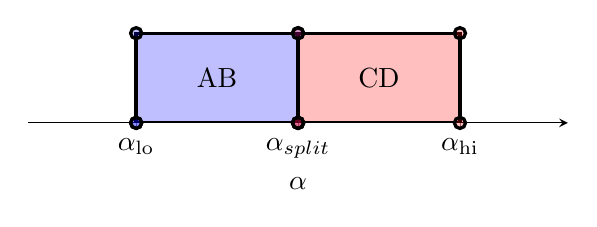
\begin{tikzpicture}
\begin{axis}[
    xmin=0, xmax=1,
    axis x line=bottom,% only show the bottom x axis
    xlabel={$\alpha$},
    xtick={0.2,0.5,0.8},
    xticklabels={$\alo$,$\alpha_{split}$,$\ahi$},
    hide y axis,    
    ymin=0,ymax=5,
    scatter/classes={%
        a={mark=o,draw=black}}
    ]

    \addplot [mark=*,very thick,fill=blue, fill opacity=0.25] coordinates {
        (0.2, 0)
        (0.2, 1)
        (0.5, 1)
        (0.5, 0)
        (0.2, 0)
    };
    \addplot [mark=*,very thick,fill=red, fill opacity=0.25] coordinates {
        (0.5, 0)
        (0.5, 1)
        (0.8, 1)
        (0.8, 0)
        (0.5, 0)
    };
    \node[] at (axis cs: 0.35,0.5) {AB};
    \node[] at (axis cs: 0.65,0.5) {CD};
\end{axis}
\end{tikzpicture}
\end{minipage}
\begin{minipage}{.45\textwidth}
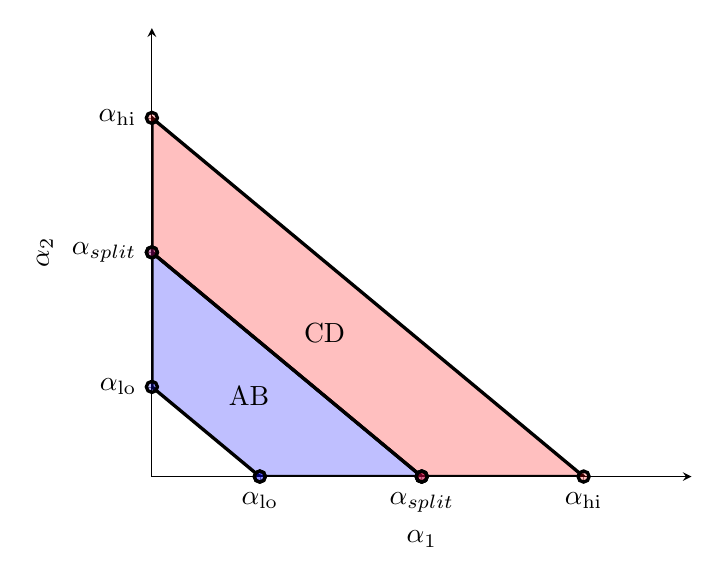
\begin{tikzpicture}
\begin{axis}[
    xmin=0, xmax=1,
    axis x line=bottom,% only show the bottom x axis
    axis y line=left,
    xlabel={$\alpha_1$},
    ylabel={$\alpha_2$},
    xtick={0.2,0.5,0.8},
    xticklabels={$\alo$,$\alpha_{split}$,$\ahi$},  
    ytick={0.2,0.5,0.8},
    yticklabels={$\alo$,$\alpha_{split}$,$\ahi$},  
    ymin=0,ymax=1,
    scatter/classes={%
        a={mark=o,draw=black}}
    ]

    \addplot [mark=*,very thick,fill=blue, fill opacity=0.25] coordinates {
        (0.2, 0)
        (0.5, 0)
        (0, 0.5)
        (0, 0.2)
        (0.2, 0)
    };
    \addplot [mark=*,very thick,fill=red, fill opacity=0.25] coordinates {
        (0.5, 0)
        (0.8, 0)
        (0, 0.8)
        (0, 0.5)
        (0.5, 0)
    };
    \node[] at (axis cs: 0.18,0.18) {AB};
    \node[] at (axis cs: 0.32,0.32) {CD};
\end{axis}
\end{tikzpicture}
\end{minipage}
\caption{While in this work, the split between different merges was based on a linear function $d(\alpha)$ (left), it will be more difficult to evaluate the merges when interpolating with two weight parameters $\alpha_1$ and $\alpha_2$, where the merges will be represented as a convex hull in the $\alpha_1$-$\alpha_2$-space (right).}
\label{fig:convexhull}
\end{figure}

\begin{figure}[h]
\centering
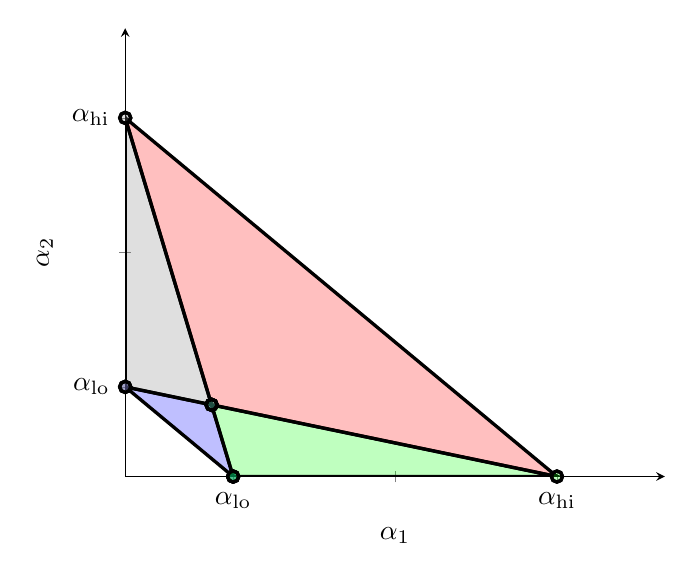
\begin{tikzpicture}
\begin{axis}[
    xmin=0, xmax=1,
    axis x line=bottom,% only show the bottom x axis
    axis y line=left,
    xlabel={$\alpha_1$},
    ylabel={$\alpha_2$},
    xtick={0.2,0.5,0.8},
    xticklabels={$\alo$,,$\ahi$},  
    ytick={0.2,0.5,0.8},
    yticklabels={$\alo$,,$\ahi$},  
    ymin=0,ymax=1,
    scatter/classes={%
        a={mark=o,draw=black}}
    ]
    \addplot [mark=*,very thick,fill=blue, fill opacity=0.25] coordinates {
        (0.2, 0)
        (0, 0.2)
        (0.16, 0.16)
        (0.2, 0)
    };
    \addplot [mark=*,very thick,fill=green, fill opacity=0.25] coordinates {
        (0.2, 0)
        (0.8, 0)
        (0.16, 0.16)
        (0.2, 0)
    };
    \addplot [mark=*,very thick,fill=gray, fill opacity=0.25] coordinates {
        (0, 0.2)
        (0, 0.8)
        (0.16, 0.16)
        (0, 0.2)
    };
    \addplot [mark=o,very thick,fill=red, fill opacity=0.25] coordinates {
        (0.16, 0.16)
        (0.8, 0)
        (0, 0.8)
        (0.16, 0.16)
    };
\end{axis}
\end{tikzpicture}
\caption{Finding the merges in the different regions can be more challenging when interpolating with two weight parameters $\alpha_1$ and $\alpha_2$.}
\label{fig:convexhulls2}
\end{figure}

In addition, we can apply the introduced algorithms to more datasets and data domains, such as the sets contained in the UCI Machine Learning Repository \cite{Dua:2019}. For instance, we could compare different datasets within one specific data domain. Say we evaluate a variety of different image datasets and compare the optimal values of $\alpha$. An interesting observation would be, if we could reuse the optimal parameter from different datasets within the same or even across other domains. In our experiments, we often found similar optimal values in the range $[0.7,0.9]$ while other ranges mostly did not lead to good results (e.g.\ $[0.0, 0.5]$). We could use this knowledge for further experiments by e.g. evaluating only smaller regions or by putting more emphasis on given parameters in general. We can then also evaluate other domains, such as (partially) labeled voice datasets (e.g. the Free Music Archive dataset \cite{fma} or LibriSpeech \cite{librispeech}) and compare the results across different data domains.\\

Also, we can imagine applying this framework to (a) other clustering algorithms than agglomerative hierarchical clustering and (b) other tasks than clustering.

% %\input{Chapters/Chapter4} % Experiment 1

% %\input{Chapters/Chapter5} % Experiment 2

% %\input{Chapters/Chapter6} % Results and Discussion

% %\input{Chapters/Chapter7} % Conclusion

% %% ----------------------------------------------------------------
% % Now begin the Appendices, including them as separate files

% \addtocontents{toc}{\vspace{2em}} % Add a gap in the Contents, for aesthetics

% \appendix % Cue to tell LaTeX that the following 'chapters' are Appendices

% \chapter{The Hungarian Method}
\label{sec:hungarian}

Our goal is to find the best possible matching between two clusterings $C_1^i, ..., C_k^i$ and $C_1^j, ..., C_k^j$. In order to do so, we calculate the cost of matching each possible pair of clusters within the two clusterings. 
% Table \ref{app:hung:distances} shows how such a cost matrix can look like.

% \begin{table}[h]
%     \centering
%     \begin{tabular}{|l | l l l l l|}
%     \hline
%     j\textbackslash i & 1 & 2 & 3 & 4 & 5\\ \hline
%     1 & 20 & 15 & 30 & 50 & 40\\
%     2 & 80 & 10 & 15 & 20 & 30\\
%     3 & 20 & 30 & 50 & 80 & 60\\
%     4 & 30 & 50 & 40 & 20 & 10\\
%     5 & 20 & 30 & 40 & 50 & 25\\ \hline
%     \end{tabular}
%     \caption{In order to determine the optimal matching between two clusterings, we note the pairwise matching costs.}
%     \label{app:hung:distances}
% \end{table}

To find the optimal matching in a brute force way, we have to look at each possible matching. Say we want to match each $i$ to one $j$. For $i = 1$ we can pick from 5 different values of $j$, for $i = 2$ there are 4 potential values of $j$. This will overall result in $k! = 5! = 120$ different combinations, thus the complexity of the brute force approach is $O(k!)$. A more efficient algorithm (especially for higher values of $k$) was introduced by Kuhn and Munkres \cite{kuhn1955hungarian}\cite{munkres1957algorithms}. It consists of three major steps. In the first one, we subtract the row minima from each row. This step is performed in table \ref{app:hung:step1}.

\begin{table}[h]
    \centering
    \begin{tabular}{|l | l l l l l| l |}
    \hline
    j\textbackslash i & 1 & 2 & 3 & 4 & 5 & \\ \hline
    1 & 5 & 0 & 15 & 35 & 25 & (-15)\\
    2 & 70 & 0 & 5 & 10 & 20 & (-10)\\
    3 & 0 & 10 & 30 & 60 & 40 & (-20)\\
    4 & 20 & 40 & 30 & 10 & 0 & (-10)\\
    5 & 0 & 10 & 20 & 30 & 5 & (-20)\\ \hline
    \end{tabular}
    \caption{Hungarian method step 1: Subtract the row minima from each row.}
    \label{app:hung:step1}
\end{table}

After subtracting the row minima, we now also subtract the column minima from each column as shown in table \ref{app:hung:step2}.

\begin{table}[h]
    \centering
    \begin{tabular}{|l | l l l l l |}
    \hline
    j\textbackslash i & 1 & 2 & 3 & 4 & 5\\ \hline
    1 & 5 & 0 & 10 & 25 & 25\\
    2 & 70 & 0 & 0 & 0 & 20\\
    3 & 0 & 10 & 25 & 50 & 40\\
    4 & 20 & 40 & 25 & 0 & 0\\
    5 & 0 & 10 & 15 & 20 & 5\\ \hline
    & - & - & (-5) & (-10) & -\\ \hline
    \end{tabular}
    \caption{Hungarian method step 2: Subtract the column minima from each column.}
    \label{app:hung:step2}
\end{table}

Now we try to find the optimal matching. To do so, we cover all zeros with lines and count the minumum needed lines to do so. Table \ref{app:hung:step3} shows that we need four lines.

\begin{table}[h]
    \centering
    \begin{tabular}{|l | l l l l l |}
    \hline
    j\textbackslash i & 1 & 2 & 3 & 4 & 5\\ \hline
    1 & \cellcolor{orange!25}5 & \cellcolor{orange!50}0 & 10 & 25 & 25\\
    2 & \cellcolor{orange!75}70 & \cellcolor{orange!75}0 & \cellcolor{orange!75}0 & \cellcolor{orange!75}0 & \cellcolor{orange!75}20\\
    3 & \cellcolor{orange!25}0 & \cellcolor{orange!50}10 & 25 & 50 & 40\\
    4 & \cellcolor{orange!75}20 & \cellcolor{orange!75}40 & \cellcolor{orange!75}25 & \cellcolor{orange!75}0 & \cellcolor{orange!75}0\\
    5 & \cellcolor{orange!25}0 & \cellcolor{orange!50}10 & 15 & 20 & 5\\ \hline
    \end{tabular}
    \caption{Hungarian method step 3: Cover all zeros with as few lines as possible.}
    \label{app:hung:step3}
\end{table}

After covering the zeros and counting the lines, we found the optimal matching in case the number of lines equals the number of rows (or columns) in the matrix. As we need four lines and the matrix has five rows in this example, we have to add more zeros. To do that, we subtract the minimum value of the matrix (which is 5 here) from all uncovered values that are not zero and add it to all values that are not zero and covered twice. Now we can again check the needed lines as in table \ref{app:hung:additionalstep}.

\begin{table}[h]
    \centering
    \begin{tabular}{|l | l l l l l |}
    \hline
    j\textbackslash i & 1 & 2 & 3 & 4 & 5\\ \hline
    1 & 5 & 0 & 5 & 20 & 20\\
    2 & 75 & 0 & 0 & 0 & 20\\
    3 & 0 & 10 & 20 & 45 & 35\\
    4 & 25 & 45 & 25 & 0 & 0\\
    5 & 0 & 10 & 10 & 15 & 0\\ \hline
    \end{tabular}
    \begin{tabular}{|l | l l l l l |}
        \hline
        j\textbackslash i & 1 & 2 & 3 & 4 & 5\\ \hline
        1 & \cellcolor{orange!25}5 & \cellcolor{orange!50}0 & 5 & 20 & 20\\
        2 & \cellcolor{orange!75}75 & \cellcolor{orange!75}0 & \cellcolor{orange!75}0 & \cellcolor{orange!75}0 & \cellcolor{orange!75}20\\
        3 & \cellcolor{orange!25}0 & \cellcolor{orange!50}10 & 20 & 45 & 35\\
        4 & \cellcolor{orange!75}25 & \cellcolor{orange!75}45 & \cellcolor{orange!75}25 & \cellcolor{orange!75}0 & \cellcolor{orange!75}0\\
        5 & \cellcolor{orange!100}0 & \cellcolor{orange!100}10 & \cellcolor{orange!100}10 & \cellcolor{orange!100}15 & \cellcolor{orange!100}0\\ \hline
    \end{tabular}
    \caption{Hungarian method additional step: Create more zeroes until the number of minimal needed lines to cover all zeros matches the number of rows.}
    \label{app:hung:additionalstep}
\end{table}

This will then result in the assignment seen in table \ref{app:hung:assignment}. Applying the matching to the input matrix then gives the optimal cost by summing the optimal values. For this example the optimal cost is then 95.

\begin{table}[h]
    \centering
    \begin{tabular}{|l | l l l l l |}
    \hline
    j\textbackslash i & 1 & 2 & 3 & 4 & 5\\ \hline
    1 & 5 & \cellcolor{blue!25}0 & 5 & 20 & 20\\
    2 & 75 & 0 & \cellcolor{blue!25}0 & 0 & 20\\
    3 & \cellcolor{blue!25}0 & 10 & 20 & 45 & 35\\
    4 & 25 & 45 & 25 & \cellcolor{blue!25}0 & 0\\
    5 & 0 & 10 & 10 & 15 & \cellcolor{blue!25}0\\ \hline
    \end{tabular}
    \begin{tabular}{|l | l l l l l|}
        \hline
        j\textbackslash i & 1 & 2 & 3 & 4 & 5\\ \hline
        1 & 20 & \cellcolor{blue!25}15 & 30 & 50 & 40\\
        2 & 80 & 10 & \cellcolor{blue!25}15 & 20 & 30\\
        3 & \cellcolor{blue!25}20 & 30 & 50 & 80 & 60\\
        4 & 30 & 50 & 40 & \cellcolor{blue!25}20 & 10\\
        5 & 20 & 30 & 40 & 50 & \cellcolor{blue!25}25\\ \hline
    \end{tabular}
    \caption{Result of the Hungarian method: The optimal matching between two clusterings.}
    \label{app:hung:assignment}
\end{table}	% Appendix Title

% \chapter{Proposed NELL Subcategories}
\label{sec:nellsubcategories}

\begin{table}[H]
  \makebox[\textwidth][c]{
  \small
  \begin{tabular}{cccc}
    \hline\hline
    \textbf{Luxury Room} & \textbf{Bathroom} & \textbf{Guest Room} & \textbf{Suite} \\ \hline
    spacious living room & large ensuite bathroom & elegant rooms & luxurious suites\\
    comfortable living room & spacious marble bathroom & three guest rooms & one bedroom suites\\
    guest room & one bathroom & large guest rooms & spacious suites\\
    lounge room & full bathroom & deluxe guest rooms & deluxe suites\\
    living room & upstairs bathroom & guests rooms & guest suites\\
    superior room & large bathroom & spacious air conditioned rooms & bedroom suites\\
    sleeping room & ensuite bathroom & furnished guest rooms & whirlpool suites\\
    main bedroom & elegant bathroom & comfortable guest rooms & three suites\\
    \hline
  \end{tabular}
  }
  \caption{Proposed Subcategories for ``Office Building Room''.}
  \label{tbl:rooms}
\end{table}

\begin{table}[H]
  \makebox[\textwidth][c]{
  \small
  \begin{tabular}{ccccc}
    \hline\hline
    \textbf{Shoes} & \textbf{Uniform/Costume} & \textbf{Pants} & \textbf{Casual} & \textbf{Specialized} \\ \hline
    shoes & costume & kneepants & stocking cap & long stockings\\
    high heel shoes & work uniforms & baggy pants & workout clothes & wide brimmed hat\\
    sensible shoes & outfits & loose fitting pants & casual clothes & casual wear\\
    old shoes & period costume & slacks & baseball caps & black stockings\\
    pointe shoes & folk costumes & black shorts & skull caps & wear socks\\
    dark shoes & halter top & special clothing & ball caps & high heels\\
    spira shoes & period costumes & white shorts & evening clothes & surf wear\\
    mens shoes & costumes & underpants & ball cap & wear gloves\\
    \hline
  \end{tabular}
  }
  \caption{Proposed Subcategories for ``Clothing''.}
  \label{tbl:clothing}
\end{table}

\begin{table}[H]
  \makebox[\textwidth][c]{
  \small
  \begin{tabular}{cccc}
    \hline\hline
    \textbf{Stove/Oven} & \textbf{Machines} & \textbf{Bowls} & \textbf{Baking Sheets} \\ \hline
    full size stove & cookie cutters & large mixing bowl & oiled baking sheet\\
    full size cooker & automatic washing machine & large serving bowl & rimmed baking sheet\\
    red hot stove & washing machine & small bowl & large baking sheet\\
    plastic jug & bread machine & single bowl & small baking sheet\\
    toaster & cookie cutter & separate bowl & prepared baking sheet\\
    greased baking dish & coffee machine & shallow bowl & ungreased baking sheet\\
    wood burning pizza oven & cooking spray & separate mixing bowl & hot plate\\
    ceramic top stove & coffee grinder & large bowl & greased baking sheet\\
    \hline
  \end{tabular}
  }
  \caption{Proposed Subcategories for ``Kitchen Item''.}
  \label{tbl:kitchenitems}
\end{table} % Appendix Title

% %\chapter{Additional NELL Results}
\label{app:nell}

Here we show the results of all the 32 different used entities. We used a maximum of 1,000 points for each entity, however for some of them less samples were given. We show both interpolating between average and complete and between single and complete linkage in the following figures.

\begin{figure}[h]
\centering
\begin{minipage}{.24\textwidth}
  \centering
  \subcaptionbox{Animal}
  {\includegraphics[width=\linewidth]{plots/nell-ac/animal}}
\end{minipage}
\begin{minipage}{.24\textwidth}
  \centering
  \subcaptionbox{Arthropod}
  {\includegraphics[width=\linewidth]{plots/nell-ac/arthropod}}
\end{minipage}
\begin{minipage}{.24\textwidth}
  \centering
  \subcaptionbox{Attraction}
  {\includegraphics[width=\linewidth]{plots/nell-ac/attraction}}
\end{minipage}
\begin{minipage}{.24\textwidth}
  \centering
  \subcaptionbox{Beverage}
  {\includegraphics[width=\linewidth]{plots/nell-ac/beverage}}
\end{minipage}
\begin{minipage}{.24\textwidth}
  \centering
  \subcaptionbox{Bodypart}
  {\includegraphics[width=\linewidth]{plots/nell-ac/bodypart}}
\end{minipage}
\begin{minipage}{.24\textwidth}
  \centering
  \subcaptionbox{Building}
  {\includegraphics[width=\linewidth]{plots/nell-ac/building}}
\end{minipage}
\begin{minipage}{.24\textwidth}
  \centering
  \subcaptionbox{Company}
  {\includegraphics[width=\linewidth]{plots/nell-ac/company}}
\end{minipage}
\begin{minipage}{.24\textwidth}
  \centering
  \subcaptionbox{Creative Work}
  {\includegraphics[width=\linewidth]{plots/nell-ac/creativework}}
\end{minipage}
\begin{minipage}{.24\textwidth}
  \centering
  \subcaptionbox{Date}
  {\includegraphics[width=\linewidth]{plots/nell-ac/date}}
\end{minipage}
\begin{minipage}{.24\textwidth}
  \centering
  \subcaptionbox{Event}
  {\includegraphics[width=\linewidth]{plots/nell-ac/event}}
\end{minipage}
\begin{minipage}{.24\textwidth}
  \centering
  \subcaptionbox{Food}
  {\includegraphics[width=\linewidth]{plots/nell-ac/food}}
\end{minipage}
\begin{minipage}{.24\textwidth}
  \centering
  \subcaptionbox{Fruit}
  {\includegraphics[width=\linewidth]{plots/nell-ac/fruit}}
\end{minipage}
\begin{minipage}{.24\textwidth}
  \centering
  \subcaptionbox{Game}
  {\includegraphics[width=\linewidth]{plots/nell-ac/game}}
\end{minipage}
\begin{minipage}{.24\textwidth}
  \centering
  \subcaptionbox{Household Item}
  {\includegraphics[width=\linewidth]{plots/nell-ac/householditem}}
\end{minipage}
\begin{minipage}{.24\textwidth}
  \centering
  \subcaptionbox{Invertebrate}
  {\includegraphics[width=\linewidth]{plots/nell-ac/invertebrate}}
\end{minipage}
\begin{minipage}{.24\textwidth}
  \centering
  \subcaptionbox{Location}
  {\includegraphics[width=\linewidth]{plots/nell-ac/location}}
\end{minipage}
\end{figure}
\begin{figure}[h]\ContinuedFloat
\centering
\begin{minipage}{.24\textwidth}
  \centering
  \subcaptionbox{Mediacompany}
  {\includegraphics[width=\linewidth]{plots/nell-ac/mediacompany}}
\end{minipage}
\begin{minipage}{.24\textwidth}
  \centering
  \subcaptionbox{Organization}
  {\includegraphics[width=\linewidth]{plots/nell-ac/organization}}
\end{minipage}
\begin{minipage}{.24\textwidth}
  \centering
  \subcaptionbox{Person}
  {\includegraphics[width=\linewidth]{plots/nell-ac/person}}
\end{minipage}
\begin{minipage}{.24\textwidth}
  \centering
  \subcaptionbox{Person by Location}
  {\includegraphics[width=\linewidth]{plots/nell-ac/personbylocation}}
\end{minipage}
\begin{minipage}{.24\textwidth}
  \centering
  \subcaptionbox{Person NA}
  {\includegraphics[width=\linewidth]{plots/nell-ac/personnorthamerica}}
\end{minipage}
\begin{minipage}{.24\textwidth}
  \centering
  \subcaptionbox{Physiological Condition}
  {\includegraphics[width=\linewidth]{plots/nell-ac/physiologicalcondition}}
\end{minipage}
\begin{minipage}{.24\textwidth}
  \centering
  \subcaptionbox{Politics Group}
  {\includegraphics[width=\linewidth]{plots/nell-ac/politicsgroup}}
\end{minipage}
\begin{minipage}{.24\textwidth}
  \centering
  \subcaptionbox{Product}
  {\includegraphics[width=\linewidth]{plots/nell-ac/Product}}
\end{minipage}
\begin{minipage}{.24\textwidth}
  \centering
  \subcaptionbox{Publication}
  {\includegraphics[width=\linewidth]{plots/nell-ac/publication}}
\end{minipage}
\begin{minipage}{.24\textwidth}
  \centering
  \subcaptionbox{School}
  {\includegraphics[width=\linewidth]{plots/nell-ac/school}}
\end{minipage}
\begin{minipage}{.24\textwidth}
  \centering
  \subcaptionbox{Software}
  {\includegraphics[width=\linewidth]{plots/nell-ac/software}}
\end{minipage}
\begin{minipage}{.24\textwidth}
  \centering
  \subcaptionbox{Sports Event}
  {\includegraphics[width=\linewidth]{plots/nell-ac/sportsevent}}
\end{minipage}
\begin{minipage}{.24\textwidth}
  \centering
  \subcaptionbox{Traditional Game}
  {\includegraphics[width=\linewidth]{plots/nell-ac/traditionalgame}}
\end{minipage}
\begin{minipage}{.24\textwidth}
  \centering
  \subcaptionbox{Vertebrate}
  {\includegraphics[width=\linewidth]{plots/nell-ac/vertebrate}}
\end{minipage}
\begin{minipage}{.24\textwidth}
  \centering
  \subcaptionbox{Visualizable Attribute}
  {\includegraphics[width=\linewidth]{plots/nell-ac/visualizableattribute}}
\end{minipage}
\begin{minipage}{.24\textwidth}
  \centering
  \subcaptionbox{Website}
  {\includegraphics[width=\linewidth]{plots/nell-ac/website}}
\end{minipage}
\caption{Interpolating between average and complete linkage for the NELL data.}
\end{figure}

\begin{figure}[h]
\centering
\begin{minipage}{.24\textwidth}
  \centering
  \subcaptionbox{Animal}
  {\includegraphics[width=\linewidth]{plots/nell-sc/animal}}
\end{minipage}
\begin{minipage}{.24\textwidth}
  \centering
  \subcaptionbox{Arthropod}
  {\includegraphics[width=\linewidth]{plots/nell-sc/arthropod}}
\end{minipage}
\begin{minipage}{.24\textwidth}
  \centering
  \subcaptionbox{Attraction}
  {\includegraphics[width=\linewidth]{plots/nell-sc/attraction}}
\end{minipage}
\begin{minipage}{.24\textwidth}
  \centering
  \subcaptionbox{Beverage}
  {\includegraphics[width=\linewidth]{plots/nell-sc/beverage}}
\end{minipage}
\begin{minipage}{.24\textwidth}
  \centering
  \subcaptionbox{Bodypart}
  {\includegraphics[width=\linewidth]{plots/nell-sc/bodypart}}
\end{minipage}
\begin{minipage}{.24\textwidth}
  \centering
  \subcaptionbox{Building}
  {\includegraphics[width=\linewidth]{plots/nell-sc/building}}
\end{minipage}
\begin{minipage}{.24\textwidth}
  \centering
  \subcaptionbox{Company}
  {\includegraphics[width=\linewidth]{plots/nell-sc/company}}
\end{minipage}
\begin{minipage}{.24\textwidth}
  \centering
  \subcaptionbox{Creative Work}
  {\includegraphics[width=\linewidth]{plots/nell-sc/creativework}}
\end{minipage}
\begin{minipage}{.24\textwidth}
  \centering
  \subcaptionbox{Date}
  {\includegraphics[width=\linewidth]{plots/nell-sc/date}}
\end{minipage}
\begin{minipage}{.24\textwidth}
  \centering
  \subcaptionbox{Event}
  {\includegraphics[width=\linewidth]{plots/nell-sc/event}}
\end{minipage}
\begin{minipage}{.24\textwidth}
  \centering
  \subcaptionbox{Food}
  {\includegraphics[width=\linewidth]{plots/nell-sc/food}}
\end{minipage}
\begin{minipage}{.24\textwidth}
  \centering
  \subcaptionbox{Fruit}
  {\includegraphics[width=\linewidth]{plots/nell-sc/fruit}}
\end{minipage}
\begin{minipage}{.24\textwidth}
  \centering
  \subcaptionbox{Game}
  {\includegraphics[width=\linewidth]{plots/nell-sc/game}}
\end{minipage}
\begin{minipage}{.24\textwidth}
  \centering
  \subcaptionbox{Household Item}
  {\includegraphics[width=\linewidth]{plots/nell-sc/householditem}}
\end{minipage}
\begin{minipage}{.24\textwidth}
  \centering
  \subcaptionbox{Invertebrate}
  {\includegraphics[width=\linewidth]{plots/nell-sc/invertebrate}}
\end{minipage}
\begin{minipage}{.24\textwidth}
  \centering
  \subcaptionbox{Location}
  {\includegraphics[width=\linewidth]{plots/nell-sc/location}}
\end{minipage}
\begin{minipage}{.24\textwidth}
  \centering
  \subcaptionbox{Mediacompany}
  {\includegraphics[width=\linewidth]{plots/nell-sc/mediacompany}}
\end{minipage}
\begin{minipage}{.24\textwidth}
  \centering
  \subcaptionbox{Organization}
  {\includegraphics[width=\linewidth]{plots/nell-sc/organization}}
\end{minipage}
\begin{minipage}{.24\textwidth}
  \centering
  \subcaptionbox{Person}
  {\includegraphics[width=\linewidth]{plots/nell-sc/person}}
\end{minipage}
\begin{minipage}{.24\textwidth}
  \centering
  \subcaptionbox{Person by Location}
  {\includegraphics[width=\linewidth]{plots/nell-sc/personbylocation}}
\end{minipage}
\end{figure}
\begin{figure}[h]\ContinuedFloat
\centering
\begin{minipage}{.24\textwidth}
  \centering
  \subcaptionbox{Person NA}
  {\includegraphics[width=\linewidth]{plots/nell-sc/personnorthamerica}}
\end{minipage}
\begin{minipage}{.24\textwidth}
  \centering
  \subcaptionbox{Physiological Condition}
  {\includegraphics[width=\linewidth]{plots/nell-sc/physiologicalcondition}}
\end{minipage}
\begin{minipage}{.24\textwidth}
  \centering
  \subcaptionbox{Politics Group}
  {\includegraphics[width=\linewidth]{plots/nell-sc/politicsgroup}}
\end{minipage}
\begin{minipage}{.24\textwidth}
  \centering
  \subcaptionbox{Product}
  {\includegraphics[width=\linewidth]{plots/nell-sc/Product}}
\end{minipage}
\begin{minipage}{.24\textwidth}
  \centering
  \subcaptionbox{Publication}
  {\includegraphics[width=\linewidth]{plots/nell-sc/publication}}
\end{minipage}
\begin{minipage}{.24\textwidth}
  \centering
  \subcaptionbox{School}
  {\includegraphics[width=\linewidth]{plots/nell-sc/school}}
\end{minipage}
\begin{minipage}{.24\textwidth}
  \centering
  \subcaptionbox{Software}
  {\includegraphics[width=\linewidth]{plots/nell-sc/software}}
\end{minipage}
\begin{minipage}{.24\textwidth}
  \centering
  \subcaptionbox{Sports Event}
  {\includegraphics[width=\linewidth]{plots/nell-sc/sportsevent}}
\end{minipage}
\begin{minipage}{.24\textwidth}
  \centering
  \subcaptionbox{Traditional Game}
  {\includegraphics[width=\linewidth]{plots/nell-sc/traditionalgame}}
\end{minipage}
\begin{minipage}{.24\textwidth}
  \centering
  \subcaptionbox{Vertebrate}
  {\includegraphics[width=\linewidth]{plots/nell-sc/vertebrate}}
\end{minipage}
\begin{minipage}{.24\textwidth}
  \centering
  \subcaptionbox{Visualizable Attribute}
  {\includegraphics[width=\linewidth]{plots/nell-sc/visualizableattribute}}
\end{minipage}
\begin{minipage}{.24\textwidth}
  \centering
  \subcaptionbox{Website}
  {\includegraphics[width=\linewidth]{plots/nell-sc/website}}
\end{minipage}
\caption{Interpolating between single and complete linkage for the NELL data.}
\end{figure} % Appendix Title

% \addtocontents{toc}{\vspace{2em}}  % Add a gap in the Contents, for aesthetics
% \backmatter

% %% ----------------------------------------------------------------
% \label{Bibliography}
% \lhead{\emph{Bibliography}}  % Change the left side page header to "Bibliography"
% \bibliographystyle{unsrtnat}  % Use the "unsrtnat" BibTeX style for formatting the Bibliography
% \bibliography{Bibliography}  % The references (bibliography) information are stored in the file named "Bibliography.bib"

% \end{document}  % The End
% %% ----------------------------------------------------------------